\documentclass[11pt,a4paper,footinclude=true,headinclude=true,oneside]{scrbook} % KOMA-Script book
\usepackage[T1]{fontenc}                
\usepackage{lipsum}
\usepackage[linedheaders,manychapters,pdfspacing]{classicthesis} % ,manychapters
%\usepackage[osf]{libertine}
\usepackage{amsthm}

% [MQH]
\usepackage{graphicx}
\usepackage{longtable}
\usepackage{listings}
% Source: https://tex.stackexchange.com/a/179956
\usepackage{xcolor}
\lstset{
    basicstyle=\ttfamily,
    numbers=left,
    keywordstyle=\color[rgb]{0.13,0.29,0.53}\bfseries,
    stringstyle=\color[rgb]{0.31,0.60,0.02},
    commentstyle=\color[rgb]{0.56,0.35,0.01}\itshape,
    numberstyle=\footnotesize,
    stepnumber=1,
    numbersep=5pt,
    backgroundcolor=\color[RGB]{248,248,248},
    showspaces=false,
    showstringspaces=false,
    showtabs=false,
    tabsize=2,
    captionpos=b,
    breaklines=true,
    breakatwhitespace=true,
    breakautoindent=true,
    escapeinside={\%*}{*)},
    linewidth=\textwidth,
    basewidth=0.5em,
}

\begin{document}
    \begin{titlepage}
    
    \begin{center}
    \textsc{\LARGE The Implementation of Operating System Kernel with 539kernel}\\[1,5cm]
    
    
    by\\[0,5cm]
    Mohammed Q. Hussain\\[2,5cm]
    
    
    \end{center}
    
    \vfill
    
    \end{titlepage}
	\tableofcontents 
	\include{generated_tex/Introduction}
	\chapter{Chapter 1: Let's Start with the
Bootloader}\label{ch-bootloader}

\section{Introduction}\label{introduction}

The first piece to start with when writing an operating system's kernel
is the \emph{boot loader} which is the code that is responsible for
loading the main kernel from the disk to the main memory so the kernel
can be executed. Before getting started in the details of the boot
loader and all other parts of the kernel, we need to learn a little bit
about the tools (e.g.~compilers and programming languages) that we will
use in our journey of creating a kernel. In this chapter, we start with
an overview on the tools and their basics and then we start in writing a
boot loader.

\section{x86 Assembly Language
Overview}\label{x86-assembly-language-overview}

To build a boot loader, we need to use assembly language, also, there
are some parts of an operating system kernel that cannot be written in a
high-level language and assembly language should be used instead as you
will see later in this book, therefore, a basic knowledge of the target
architecture assembly is required, in our case, the target architecture
of our kernel is x86.

The program that takes a source code which is written in assembly
language and transforms this code to the machine language is known as
\emph{assembler} \footnote{While the program that transforms the source
  code which is written in high-level language such as C to machine code
  is known as \emph{compiler}.}. There are many assemblers available for
x86 but the one that we are going to use is Netwide Assembler (NASM).
However, the concepts of x86 assembly are the same, they are tight to
the architecture itself, also the instructions are the same, so if you
grasp the basics it will be easy to use any other assembler \footnote{Another
  popular open-source assembler is GNU Assembler (GAS). One of main
  differences between NASM and GAS that the first uses Intel's syntax
  while the second uses AT\&T syntax.} even if it uses other syntax than
NASM. Don't forget that the assembler is just a tool that helps us to
generate an executable x86 machine code out of an assembly code, so, any
suitable assembler that we use to reach our goal will be enough.

In this section I don't aim to examine the details of x86 or NASM, you
can consider this section as a quick start on both x86 and NASM, the
basics will be presented to make you familiar with x86 assembly
language, more advanced concepts will be presented later when we need
them. If you are interested in x86 assembly for its own sake, there are
multiple online resources and books that explain it in details.

\subsection{Registers}\label{registers}

In any processor architecture, and x86 is not an exception, a register
is a small memory inside the processor's chip. Like any other type of
memories (e.g.~RAM), we can store data inside a register and we can read
data from it, the registers are too small and too fast. The processor
architecture provides us with multiple registers. In x86 there are two
types of registers: general purpose registers and special purpose
registers. In general purpose registers we can store any kind of data we
want, while the special purpose registers are provided by the
architecture for some specific purposes, we will encounter the second
type later in our journey of creating 539kernel.

x86 provides us with eight general purpose registers and to use them in
order to read from or write to them we refer to them by their names in
assembly code. The names of these registers are: \lstinline!EAX!,
\lstinline!EBX!, \lstinline!ECX!, \lstinline!EDX!, \lstinline!ESI!,
\lstinline!EDI!, \lstinline!EBP!, and \lstinline!ESP!. While the
registers \lstinline!ESI!, \lstinline!EDI!, \lstinline!EBP! and
\lstinline!ESP! are considered as general purpose registers in x86
architecture \footnote{According to Intel's manual.}, we will see later
that they store some important data in some cases and it's better to use
them carefully if we are forced to.

The size of each one of x86's general purpose registers is
\lstinline!32! bits (\lstinline!4! bytes) and due to that, they are
available only on x86 processors that supports \lstinline!32-bit!
architecture \footnote{Also they are available on \textbf{64-bit} x86
  CPUs such as Core i7 for instance.} such as Pentium 4 for instance.
These \lstinline!32-bit! registers are not available on x86 processors
that support only \lstinline!16-bit! architecture or lower, so, for
example, you can't use the register \lstinline!EAX! in Intel 8086
because it is a \lstinline!16-bit! x86 processor and not
\lstinline!32-bit!.

In old days, when \lstinline!16-bit! x86 processors were dominant,
assembly programmers used the registers \lstinline!AX!, \lstinline!BX!,
\lstinline!CX! and \lstinline!DX! and each one of them is of size
\lstinline!16! bits (\lstinline!2! bytes), but when \lstinline!32-bit!
x86 processors came, these registers have been extended to have the size
\lstinline!32-bit! and their names were changed to \lstinline!EAX!,
\lstinline!EBX!, \lstinline!ECX! and \lstinline!EDX!. The first letter
\lstinline!E! of the new names means \emph{extended}. However, the old
names are still usable in \lstinline!32-bit! x86 processors and they are
used to access and manipulate the first \lstinline!16! bits of the
corresponding register, for instance, to access the first \lstinline!16!
bits of the register \lstinline!EAX!, the name \lstinline!AX! can be
used. Furthermore, the first \lstinline!16! bits of these registers can
be divided into two parts and each one of them is of size \lstinline!8!
bits (\lstinline!1! bytes) and has its own name that can be referred to
in the assembly code. The first \lstinline!8! bits of the register are
called the \emph{low} bits, while the second \lstinline!8! bits are
called the \emph{high} bits.

Let's take one of these register as an example:\lstinline!AX! register
is a \lstinline!16-bit! register which is a part of the bigger
\lstinline!32-bit! \lstinline!EAX! register in \lstinline!32-bit!
architecture. \lstinline!AX! \footnote{Or in other words for
  \lstinline!32-bit! architecture: The first \lstinline!16! bits of
  \lstinline!EAX!.} is divided into two more parts, \lstinline!AL! for
the \textbf{l}ow \lstinline!8! bits as the second letter of the name
indicates and \lstinline!AH! for the \textbf{h}igh \lstinline!8! bits as
the second letter of the name indicates. The same division holds true
for the registers \lstinline!BX!, \lstinline!CX! and \lstinline!DX!,
figure \ref{fig:26012022_0} illustrates that division.

\begin{figure}
\centering
\includegraphics[width=0.50000\textwidth]{Figures/bootloader-ch/Fig26012022_0.png}
\caption{How the Registers \lstinline!EAX!, \lstinline!EBX!,
\lstinline!ECX! and \lstinline!EDX! are Divided in
x86}\label{fig:26012022_0}
\end{figure}

\subsection{Instruction Set}\label{instruction-set}

The processor's architecture provides the programmer with a bunch of
\emph{instructions} that can be used in assembly code. Processor's
instructions resemble functions \footnote{Or a procedure for people who
  work with Algol-like programming languages.} in a high-level languages
which are provided by the libraries, in our case, we can consider the
processor as the ultimate library for the assembly code. As with
functions in high-level programming languages, each instruction has a
name and performs a specific job, also, it can take parameters which are
called \emph{operands}. Depending on the instruction itself, the
operands can be a static value (e.g.~a number), a register name that the
instruction is going to fetch the stored value of it to be used or even
a memory location.

The assembly language is really simple. An assembly code is simply a
sequence of instructions which will be executed sequentially. The
following is an example of assembly code, don't worry about its
functionality right now, you will understand what it does eventually.

\begin{lstlisting}
mov ah, 0Eh
mov al, 's' 
int 10h
\end{lstlisting}

As you can see, each line starts with an instruction which is provided
to us by x86 architecture, in the first two lines we use an instruction
named \lstinline!mov! and as you can see, this instruction receives two
operands which are separated by a comma. In the current usage of this
instruction we can see that the first operand is a register name while
the second operand is a static value. The third line uses another
instruction named \lstinline!int! which receives one operand. When this
code is running, it will be executed by the processor sequentially,
starting from the first line until it finishes in the last line.

If you are interested on the available instructions on x86, there is a
four-volumes manual named ``Intel® 64 and IA-32 architectures software
developer's manual'' provided by Intel that explains each instruction in
details \footnote{\url{https://software.intel.com/en-us/articles/intel-sdm}}.

\subsubsection{\texorpdfstring{Assigning Values with
\texttt{mov}}{Assigning Values with mov}}\label{assigning-values-with-mov}

You can imagine a register as a variable in high-level languages. We can
assign values to a variable, we can change its old value and we can copy
its value to another variable. In assembly language, these operations
can be performed by the instruction \lstinline!mov! which takes the
value of the second operand and stores it in the first operand. You have
seen in the previous examples the following two lines that use
\lstinline!mov! instruction.

\begin{lstlisting}
mov ah, 0Eh
mov al, 's' 
\end{lstlisting}

Now you can tell that the first line copies the value \lstinline!0Eh! to
the register \lstinline!ah!, and the second line copies the character
\lstinline!s! to the register \lstinline!al!. The single quotation is
used in NASM to represent strings or characters and that's why we have
used it in the second line, based on that, you may noticed that the
value \lstinline!0Eh! is not surrounded by a single quotation though it
contains characters, in fact, this value isn't a string, it is a number
that is represented by hexadecimal numbering system and due to that the
character \lstinline!h! was put in the end of that value, that is,
putting \lstinline!h! in the end of \lstinline!0E! tells NASM that this
value is a hexadecimal number, the equivalent number of \lstinline!0E!
in the decimal numbering system, which we humans are using, is
\lstinline!14!, that is \lstinline!0E! and \lstinline!14! are the
exactly the same, but they are represented in two different numbering
system\footnote{Numbering systems will be discussed in more details
  later.}.

\subsection{NASM}\label{nasm}

Netwide Assembler (NASM) is an open-source assembler for x86
architecture which uses Intel's syntax of assembly language, the other
well-known syntax for assembly language is AT\&T syntax and, of course,
there are some differences between the two, the first syntax is used in
the official manuals of Intel. NASM can be used through command line to
assemble \footnote{The process of transforming an assembly source code
  to machine code is known as \emph{assembling}.} x86 assembly code and
generate the corresponding machine code. The basic usage of NASM command
is the following.

\begin{lstlisting}
nasm -f <format> <filename> [-o <output>]
\end{lstlisting}

The argument \lstinline!format! decides the binary format of the
generated machine code, the binary format will be discussed in more
details in a moment. The second argument is the \lstinline!filename! of
the assembly file that we would like to assemble, and the last option
and argument are optional, we use them if we want to specify a specific
name for the generated binary file, the default name will be same as the
filename with a different extension.

\subsubsection{Binary Format}\label{binary-format}

A \emph{binary format} is basically a specification which gives a
blueprint of how a binary file is organized, in other words, it
describes how a binary file is structured, in general there are multiple
parts in a binary file and a binary format can be used format them, the
machine code is one part of a binary file parts. Note that each
executable file uses some binary format to organize its content and to
make a specific operating system understands its content. There is no
difference between the programming languages in the matter of the binary
format \footnote{Of course the programming language should be a
  \emph{compiled} programming language such as C and Rust and not an
  \emph{interpreted} such as Python or a one that uses a virtual machine
  such as Java.} that will be used in the last output of the compiling
process, for example in Linux, if we create a software either by C, Rust
or assembly, the last executable result will be a binary file that is
formatted by using a binary format known as \emph{Executable and
Linkable Format} (ELF) which is the default in Linux. There are many
other binary formats, Mach-O is one example which is used by Mach-based
\footnote{Mach is an operating system's kernel which is well-known for
  using \emph{microkernel} design. It has been started as a research
  effort in Carnegie Mellon University in 1985. Current Apple's
  operating systems macOS and iOS are both based on an older operating
  system known as NeXTSTEP which used Mach as its kernel,}, another
example is Portable Executable (PE) which is used by Microsoft Windows.

Each operating system knows its own binary format well, and knows how a
binary file that uses this format is structured, and how to seek the
binary file to find the machine code that should be loaded into memory
and executed by the processor. For example, when you run an ELF
executable file in GNU/Linux system, the Linux kernel knows it is an ELF
executable file and assumes that it is organized in a specific way, by
using the specification of ELF, Linux kernel will be able to locate the
machine code of the software inside the ELF file and load it into memory
to be ready for execution.

In any binary format, one major part of the binary file that uses this
format is the machine code that has been produced by compiling or
assembling some source code, the machine code is specific to a processor
architecture, for example, the machine code that has been generated for
x64 \footnote{The x86 architecture that supports 64-bit.} cannot run on
x86. Because of that the binary files are distributed according to the
processor architecture which can run on, for example, GNU/Linux users
see the names of software packages in the following format
\lstinline!nasm_2.14-1_i386.deb!, the part \lstinline!i386! tells the
users that the binary machine code of this package is generated for
\lstinline!i386! architecture, which is another name for x86 by the way,
that means this package cannot be used in a machine that uses ARM
processor such as Raspberry Pi for example.

Due to that, to distribute a binary file of the same software for
multiple processor's architectures, a separate binary file should be
generated for each architecture, to solve this problem, a binary format
named \lstinline!FatELF! was presented. In this binary format, the
software machine code of multiple processor architectures are gathered
in one binary file and the suitable machine code will be loaded and run
based on the type of the system's processor. Naturally, the size of the
files that use such format will be bigger than the files that uses a
binary format that is oriented for one processor architecture. Due to
the bigger size, this type of binary formats is known as \emph{fat
binary}.

Getting back to the \lstinline!format! argument of NASM, if our goal of
using assembly language is to produce an executable file for Linux for
example, we will use \lstinline!elf! as a value for \lstinline!format!
argument. But we are working with low-level kernel development, so our
binary files should be flat and the value of \lstinline!format! should
be \lstinline!bin! to generate a \emph{flat binary} file which doesn't
use any specification, instead, in flat binary files, the output is
stored as is with no additional information or organization, only the
output machine language of our code. Using flat binary for bootloader
does make sense and that's because the code which is going to load
\footnote{Which is BIOS as we will see later.} our binary file doesn't
understand any binary format to interpret it and fetch the machine code
out of it, instead, the content of the binary file will be loaded to the
memory as is.

\section{GNU Make}\label{gnu-make}

GNU Make is a build automation tool. Well, don't let this fancy term
make you panic! the concept behind it is too simple. When we create a
kernel of an operating system \footnote{Or any software with any other
  compiled programming languages.} we are going to write some assembly
code and C code and both of them need to be assembled and compiled (for
the C code) to generate the machine code as binary files out of them.
With each time a modification is made in the source code, you need to
recompile (or reassemble) the code over and over again through writing
the same commands in the terminal in order to generate the last binary
output of your code. Beside the compiling and recompiling steps, an
important step needs to take place in order to generate the last output,
this operation is known as \emph{linking}, usually a programming project
contains multiple source files that call each other, compiling each one
of these files is going to generate a separate \emph{object file}
\footnote{An object file is a machine code of a source file and it is
  generated by the compiler. The object file is not an executable file
  and in our case at least it is used to be linked with other object
  files to generate the final executable file.} for each one, in linking
process these different object files are linked with each other to
generate one binary file out of these multiple object files, this last
binary file represents the program that we are writing.

These operations which are needed to generate the last binary file out
of the source code is known as \emph{building process}, which, as
mentioned earlier, involves executing multiple commands such as
compiling, assembling and linking. The building process a tedious job
and error-prone and to save our time (and ourselves from boredom of
course) we don't want to write all these commands over and over again in
order to generate the last output, we need an alternative and here where
GNU Make \footnote{And any other building automation tool.} comes to the
rescue, it \emph{automates} the \emph{building} process by gathering all
required commands in a text file known as \lstinline!Makefile! and once
the user runs this file through the command \lstinline!make!, GNU Make
is going to run these commands sequentially, furthermore, it checks
whether a code file is modified since the last building process or not,
if the case is that the file is not modified then it will not be
compiled again and the generated object file from the last building
process is used instead, which of course minimize the needed time to
finish the building process.

\subsection{Makefile}\label{makefile}

A \lstinline!makefile! is a text file that tells GNU Make what are the
needed steps to complete the building process of a specific source code.
There is a specific syntax that we should obey when writing
\lstinline!makefile!. A number of \emph{rules} may be defined, we can
say that a \lstinline!makefile! has a list of rules that define how to
create the executable file. Each rule has the following format:

\begin{lstlisting}[language=make]
target: prerequisites
    recipe
\end{lstlisting}

When we run the command \lstinline!make! without specifying a defined
target name as an argument, GNU Make is going to start with the first
rule in the \lstinline!makefile! only if the first rule's target name
doesn't start with dot, otherwise, the next rule will be considered. The
name of a target can be a general name or filename. Assume that we
defined a rule with the target name \lstinline!foo! and it's not the
first rule in \lstinline!makefile!, we can tell GNU Make to execute this
rule by running the command \lstinline!make foo!. One of well-known
convention when writing a \lstinline!makefile! is to define a rule with
target name \lstinline!clean! that deletes all object files and binaries
that have been created in the last building process. We will see after a
short time the case where the name of a target is a filename instead of
general name.

The \lstinline!prerequisites! part of a rule is what we can call the
list of dependencies, those dependencies can be either filenames (the C
files of the source code for instance) or other rules in the same
\lstinline!makefile!. For GNU Make, to run the a specific rule
successfully, the dependencies of this rule should be fulfilled, if
there is another rule in the dependencies, it should be executed
successfully first, if there is a filename in the dependencies list and
there is no rule that has the same filename as a target name, then this
file will be checked and used in the recipe of the rule.

Each line in the \lstinline!recipe! part should start with a tab and it
contains the commands that is going to run when the rule is being
executed. These commands are normal Linux commands, so in this part of a
rule we are going to write the compiling commands to compile the C
source files, assembling commands for the assembly source files and
linking command that links the generated object files. Any arbitrary
command can be used in the recipe as we will see later when we create
the \lstinline!makefile! of 539kernel. Consider the following C source
files, the first one is \lstinline!file1.c!, the second one is
\lstinline!file2.h! and the third one is \lstinline!file2.c!.

\begin{lstlisting}[language=C]
#include "file2.h"
int main()
{
    func();
}
\end{lstlisting}

\begin{lstlisting}[language=C]
void func();
\end{lstlisting}

\begin{lstlisting}[language=C]
#include <stdio.h>
void func()
{
    printf( "Hello World!" );
}
\end{lstlisting}

By using these three files, let's take an example of a
\lstinline!makefile! with filenames that have no rules with same
target's name.

\begin{lstlisting}[language=make]
build: file1.c file2.c
    gcc -o ex_file file1.c file2.c
\end{lstlisting}

The target name of this rule is \lstinline!build!, and since it is the
first and only rule in the \lstinline!makefile! which its name doesn't
start with a dot, then it will be executed directly once the command
\lstinline!make! is issued, another way to execute this rule is by
mentioning its name explicitly as an argument to \lstinline!make!
command as the following: \lstinline!make build!.

The rule \lstinline!build! depends on two C files, \lstinline!file1.c!
and \lstinline!file2.c!, they should be available on the same directory.
The the recipe uses GNU GCC to compile and link these two files and
generate an executable file named \lstinline!ex_file!. The following is
an example of a \lstinline!makefile! that has multiple rules.

\begin{lstlisting}[language=make]
build: file2.o file1.o
    gcc -o ex_file file1.o file2.o
file1.o: file1.c
    gcc -c file1.c
file2.o: file2.c file2.h
    gcc -c file2.c file2.h
\end{lstlisting}

In this example, the first rule \lstinline!build! depends on two object
files \lstinline!file1.o! and \lstinline!file2.o!. Before running the
building process for the first time, these two files will not be
available in the source code directory \footnote{Since they are a result
  of one step of the building process which is the compiling step that
  has not been performed yet.}, therefore, we have defined a rule for
each one of them. The rule \lstinline!file1.o! is going to generate the
object file \lstinline!file1.o! and it depends on \lstinline!file1.c!,
the object file will be simple generated by compiling
\lstinline!file1.c!. The same happens with \lstinline!file2.o! but this
rule depends on two files instead of only one.

GNU Make also supports variables which can simply be defined as the
following: \lstinline!foo = bar! and they can be used in the rules as
the following: \lstinline!$(foo)!. Let's now redefine the second
\lstinline!makefile! by using the variables.

\begin{lstlisting}[language=make]
c_compiler = gcc
buid_dependencies = file1.o file2.o
file1_dependencies = file1.c
file2_dependencies = file2.c file2.h
bin_filename = ex_file
build: $(buid_dependencies)
    $(c_compiler) -o $(bin_filename) $(buid_dependencies)
file1.o: $(file1_dependencies)
    gcc -c $(file1_dependencies)
file2.o: $(file2_dependencies)
    gcc -c $(file2_dependencies)
\end{lstlisting}

\section{The Emulators}\label{the-emulators}

While developing an operating system kernel, for sure, you will need to
run that kernel to test your code frequently. That's of course can be
done by writing the image of the kernel on a bootable device and reboot
you machine over and over again in order to run your kernel. Obviously,
this way isn't practical and needs a lot of chore work. Moreover, when a
bug shows up, it will be really hard to debug your code by using this
way. An alternative better way is to use an emulator to run your kernel
every time you need to test it.

An emulator is a software that acts like a full computer and by using it
you can run any code that require to run on a bare metal hardware. Also,
by using an emulator, everything will be virtual, for example, you can
create a virtual hard disk (that is, not real) that can be used by your
kernel, this virtual hard disk will be a normal file in you host system,
so, if anything goes wrong in your code you will not lose your data in
your main system. Furthermore, an emulator can provide you with a
debugger which will make your life a lot easier when you need to debug
your code.

There are two options for the emulator, QEMU \footnote{\url{https://www.qemu.org/}}
and Bochs \footnote{\url{https://bochs.sourceforge.io/}}. Both of them
are open source and both of them provides us with a way to run a
debugger. Personally, I liked Bochs' debugger better since it provides
an easy GUI that saves a lot of time. QEMU on the other hand, gives that
user the ability to use GNU Debugger through command line. Running a
kernel image is simple in QEMU, the following command performs that.

\begin{lstlisting}
qemu-system-x86_64 kernel.img
\end{lstlisting}

Where \lstinline!kernel.img! is the binary file of the kernel and the
bootloader. You will see later in 539kernel's \lstinline!Makefile! that
the option \lstinline!-s! is used with QEMU, it can be safely removed
but it is used to make GNU debugger able to connect to QEMU in order to
start a debugging session. Of course you can find a lot more about QEMU
in its official documentation \footnote{\url{https://www.qemu.org/docs/master/}}.

To run your kernel by using Bochs, you need to create a configuration
text file named \lstinline!bochsrc!. Each time you run Bochs it will use
this configuration file which tells Bochs the specifications of the
virtual machine that will be created, these specifications are something
about the virtual processors, their number, their available feature, the
number of available virtual disks, their options, the path of their
files and so on. Also, whether the debugger of Bochs and its GUI is
enabled or not are decided through this configuration file. This
configuration can be easily created or edited by using a command line
interface through running the command \lstinline!bochs! with no
arguments. After creating the file you can use the option
\lstinline!-f bochsrc! where \lstinline!bochsrc! is the filename of the
configuration file to run your kernel directly with no question from
Bochs about what to do.

\section{Writing the Boot Loader}\label{writing-the-boot-loader}

When a computer powers on, a piece of code named bootloader is loaded
and takes the control of the computer. Usually, the goal of the
bootloader is loading the kernel of an operating system from the disk to
the main memory and gives the kernel the control over the computer. The
firmware of a computer is the program which loads the bootloader, in
IBM-compatible computers the name of this firmware is BIOS (Basic
Input/Output System) \footnote{Before the advent of UEFI.}.

There is a place in the hard disk called \emph{boot sector}, it is the
first sector of a hard disk \footnote{As we will see later, a magnetic
  hard disk has multiple stacked \emph{platters}, each platter is
  divided into multiple \emph{tracks} and inside each track there are
  multiple \emph{sectors}.}, BIOS loads the content of the boot sector
as a first step of running the operating system. Loading the boot
sector's content means that BIOS reads the content from hard disk and
loads it into the main memory (RAM). This loaded content from the boot
sector should be the bootloader, and once its loaded into the main
memory, the processor will be able to execute it as any other code that
we use in our computers. So, the last step performed by BIOS in booting
process is giving the control to the bootloader to do whatever it wants.

Before getting started in writing 539kernel, we need to write the
bootloader that is going to load 539kernel from the disk. In
IBM-compatible PCs that uses BIOS to perform the booting process, the
size of the bootloader is limited to \lstinline!512! bytes and due to
this limited size and the need of using low-level services, the
bootloader is usually written in assembly language, also, because of
this limited size, we cannot depend on BIOS to load 539kernel instead of
the bootloader and that's because a kernel is usually bigger than
\lstinline!512! bytes, therefore, a small bootloader is loaded by BIOS
in order to load the bigger piece of code which is the kernel. The
reason of this limited size of the bootloader is because of the size of
a sector in the hard disk itself. Each sector in the hard disk has the
size of \lstinline!512! bytes and as we have mentioned, BIOS is going to
load the content of the first sector of hard disk, the boot sector,
which, of course, as any other sector its size is \lstinline!512! bytes.

Beside the bootloader's limited size, it is going to run on an \emph{x86
operating mode} known as \emph{real mode} \footnote{The concept of x86
  operating modes and the real mode will be discussed in more details
  later.}, what we need to know about that for now is that real mode is
a \lstinline!16-bit! environment, so, even if the working processor is a
\lstinline!64-bit! processor, we can only use \lstinline!16-bit!
features of the processor, such as the registers of size \lstinline!16!
bits.

The booting process is too specific to the computer architecture as we
have seen and it may differs between one architecture and another. Some
readers, especially computer science students may notice that the
academic textbooks of operating systems don't mention the bootloader or
discuss it.

\subsection{Hard Disk Structure}\label{hard-disk-structure}

A hard disk consists of multiple \emph{platters} which are stacked
together one above the other, have you ever seen a CD or a DVD? A
platter has exactly the same shape, refer to Figure \ref{fig:a-platter}.
The both surfaces (top and down) of a platter are covered by a magnetic
layer which stores the data. For each surface of a platter there is a
read/write head on it, and as you guessed, the role of this head is to
read from a surface or write to it, a head is attached to an arm. Those
arms move horizontally, back and forth, and because the other end of all
of those arms are attached to the same physical part, they will be moved
back and forth together to the same location at the same time. Figure
\ref{fig:platters-arms-heads} shows how the platters, arms and
read/write heads are assembled together.

\begin{figure}
\centering
\includegraphics[width=0.50000\textwidth]{Figures/bootloader-ch/a-platter.png}
\caption{(A) Shows a platter when we see it from the side. (B) Shows a
platter when we see it from top/down.}\label{fig:a-platter}
\end{figure}

A surface of a platter is divided into a number of tracks and each track
is divided into a number of sectors. In Figure \ref{fig:tracks-sectors}
you can see how tracks and sectors are organized on a surface, the gray
circles that have the same center (cocenteric) are the tracks, a track
consists of a smaller parts which called sectors. A sector is the
smallest unit that holds data in hard disks and as you know from our
previous discussion, the first sector in a hard disk is known as boot
sector.

\begin{figure}
\centering
\includegraphics[width=0.50000\textwidth]{Figures/bootloader-ch/platters-arms-heads.png}
\caption{Shows how the parts of a hard disk are assembled
together.}\label{fig:platters-arms-heads}
\end{figure}

When a command is sent to the hard disk to write some data on it or read
from it, at least two mechanical moves \footnote{This fancy term
  \emph{mechanical moves} means that some physical parts of hard disk
  moves physically.} are performed. The first move is taken by the arms,
they move back or forth in order to be upon the track that contains the
data we would like to read, this operation is known as \emph{seek}
operation. So, \emph{seek time} is the time needed to put a specific
track under a read/write head. After finishing the seek operation, the
read/write head will be on the right track but, also, it will be on a
random sector \footnote{Not exactly random, can you tell why?}, to reach
the sector that we would like to read from (or write to) the platter
rotates until the read/write head becomes upon the required sector. The
speed of rotation is measured by a unit known as \emph{revolutions per
minute} (RPM) and the needed time to reach the required sector is known
as \emph{rotational latency}. Finally, the data will be
\emph{transferred} from the hard disk to the main memory, the time
needed to transfer a number of bits known as \emph{transfer time}.

Let's assume as an example a hard disk that has \lstinline!3! platters,
which means it has \lstinline!6! surfaces, arms and read/write head.
When the operating system request from the hard disk to seek a specific
track, for instance track \lstinline!3!, all \lstinline!6! heads will
seek the track \lstinline!3! and when the seek operation ends, the
\lstinline!6! heads will point to the same physical position on all
\lstinline!6! surfaces, that is, the top head of the first platter and
the bottom head of it will point to that same place, but the first one
on the top while the second is on the bottom, and so on for the other
\lstinline!4! remaining heads, the collection of all these tracks that
the heads point to at some point of time is called a \emph{cylinder}.

\begin{figure}
\centering
\includegraphics[width=0.50000\textwidth]{Figures/bootloader-ch/tracks-sectors.png}
\caption{Shows Tracks and Sectors on a platter's
surface.}\label{fig:tracks-sectors}
\end{figure}

Now, based on what we know about how a hard disk works, can we imagine
what happens inside the hard disk when BIOS loads a bootloader? First,
the arms will seek the track number \lstinline!0! \footnote{I didn't
  mention that previously, but yes, the bootloader resides in track
  \lstinline!0!.}, that is, the arms move back or forth until they reach
the track \lstinline!0!, then the platter rotates until the read/write
head become upon the sector \lstinline!0!, finally, the content of
sector \lstinline!0! is transferred to the main memory.

\subsection{BIOS Services}\label{bios-services}

We are in a journey of writing an operating system kernel, which means
that we are dealing with a little bit harsh environment! Do you remember
all libraries that we are lucky to have when developing normal software
(user-space software), well, none of them are available right now! And
they will not be available until we decide to make them so and work hard
to do that. Even the simple function \lstinline!printf! of C is not
available.

But that's fine, for our luck, in this environment, where there is too
little available for us to write our code, BIOS provides us with a bunch
of useful services that we can use in real mode, so, we can use these
services in our bootloader to get things done.

BIOS services are like a group of functions in high-level languages that
is provided by some library, each function does something useful and we
deal with those functions as black boxes, we don't know what's inside
these functions but we know what they do and how to use them. So,
basically, BIOS provides us a library of functions and we are going to
use some of these functions in our bootloader.

BIOS services are divided into categories, there are video services
category, disk services category, keyboard services category and so on.
Each category is identified by a unique number called \emph{interrupt
number}. In high-level world, we witnessed the same concept but with
different mechanism, for example, C standard library provides us with
many services (functions) such as input/output functions, string
manipulation functions, mathematical functions and so on, these
functions are categorized and each category is label by the
\emph{library name}, for example, all input/output functions can be
found in \lstinline!stdio.h! and so on. In BIOS, for example, the
category of video services has the interrupt number \lstinline!10h!. As
mentioned earlier, the letter\lstinline!h! after a number means that
this number represented in hexadecimal numbering system, or for short, a
hexadecimal number. Here, \lstinline!10h! doesn't equal the decimal
number \lstinline!10!. We already said that when a hexadecimal number is
mentioned we use \lstinline!h! as a postfix, also, \lstinline!0x!
\footnote{C programming language, for instance, uses this way for
  hexadecimal numbers.} can be used as a prefix instead of
\lstinline!h!, so \lstinline!10h! and \lstinline!0x10! are equivalents.

Inside each services category, there is a bunch of services, each one
can do a specific thing and they are identified by a number. Continuing
with C analogy, a service is a function labeled by a name (e.g.
\lstinline!printf!) and this function reside in a library (e.g.
\lstinline!stdio.h!) which is same as a category of services in BIOS. As
we said, the interrupt number \lstinline!10h! represents the category of
video services, and the service of printing a character on a screen
(function) is represented by the number \lstinline!0Eh!.

Interrupts is a fundamental concept in x86 architecture. What we need to
know about them right now is that they are a way to call a specific code
which is assigned to the interrupt number and calling an interrupt in
assembly is really simple, the instruction \lstinline!int! is used as
the following: \lstinline!int 10h!. That's it! We use the instruction
\lstinline!int! and gives it the interrupt number that represent the
code that we would like to call as an operand. In this example, we are
calling the code of interrupt \lstinline!10h! which is, as we mentioned
multiple time, the category of BIOS video services. When the CPU
executes this instruction, BIOS will be called and based on the
interrupt number it will know that we want to use one of available video
services, but which one exactly!

In the previous example, we actually didn't tell BIOS which video
service we would like to use and to do that we need to specify service
number in \lstinline!ah! register before calling the interrupt.

\begin{lstlisting}
mov ah, 0Eh
int 10h
\end{lstlisting}

That's it, all the BIOS services can be used in this exact way. First we
need to know what is the interrupt number that the service belongs to,
then, we need to know the number of the service itself, we put the
service number in the register \lstinline!ah! then we call the interrupt
by its number by using \lstinline!int! instruction.

The previous code calls the service of printing a character on a screen,
but is it complete yet? Actually no, we didn't specify what is the
character that we would like to print. We need something like parameters
in high-level languages to pass additional information for BIOS to be
able to do its job. Well, lucky us! the registers are here to the
rescue.

When a BIOS service needs additional information, that is, parameters.
It expects to find these information in a specific register. For
example, the service \lstinline!0Eh! in interrupt \lstinline!10h!
expects to find the character that the user wants to print in the
register \lstinline!al!, so, the register \lstinline!al! is one of
service \lstinline!0Eh! parameters. The following code requests from
BIOS to print the character \lstinline!S! on the screen:

\begin{lstlisting}
mov ah, 0Eh
mov al, 'S'
int 10h
\end{lstlisting}

\subsection{A Little Bit More of x86 Assembly and
NASM}\label{a-little-bit-more-of-x86-assembly-and-nasm}

We need to learn a couple more things about x86 assembly to be able to
start. In NASM, each line in the source code has the following format.

\begin{lstlisting}
label: instruction operands
\end{lstlisting}

The label is optional, the operands depend on x86 instruction in use, if
it doesn't get any operand then we don't need to write them. To write
comments on NASM we begin with semi-colon and write whatever we like
after it as a comment and the rest of the source line will be considered
as a part of the comment.

A label is a way to give an instruction or a group of instructions a
meaningful name, then we can use this name in other places in the source
code to refer to this instruction/group of instructions, we can use
labels for example to call this group of instructions or to get the
starting memory address of these instructions. Sometimes, we may use
labels to make the code more readable.

We can say that a label is something like the name of a function or
variable in C, as we know a variable name in C is a meaningful name that
represents the memory address of a location in the main memory that
contains the value of a variable, the same holds true for a function
name. Labels in NASM works in the same way, under the hood it represents
a memory address. The colon in label is also optional.

\begin{lstlisting}
print_character_S_with_BIOS:
    mov ah, 0Eh
    mov al, 'S'
    int 10h
\end{lstlisting}

You can see in the code above, we gave a meaningful name for the bunch
of instructions that prints the character \lstinline!S! on the screen.
After defining this label in our source code, we can use it anywhere in
the same source code to refer to this bunch of instructions.

\begin{lstlisting}
call_video_service int 10h
\end{lstlisting}

This is another example of labels. This time we eliminated the optional
colon in label's name and the label here points to only one instruction.
Please note that extra whitespaces and new lines doesn't matter in NASM,
so, the following is equivalent to the one above.

\begin{lstlisting}
call_video_service
    int 10h
\end{lstlisting}

Consider the following code, what do you think it does?

\begin{lstlisting}
print_character_S_with_BIOS:
    mov ah, 0Eh
    mov al, 'S'

call_video_service:
    int 10h
\end{lstlisting}

Still it prints \lstinline!S! on the screen. Introducing labels in the
source code doesn't change its flow, the code will be executed
sequentially whether we used the labels or not. The sequence of
execution will not be changed by merely using labels, if we need to
change the sequence of execution we need to use other methods than
labels. You already know one of these methods which is calling an
interrupt. So, we can say that labels are more general than a variable
name or function name in C. A label is a human-readable name for a
memory location which can contain anything, code or data!

\subsubsection{Jump and Return
Unconditionally}\label{jump-and-return-unconditionally}

Let's start this section with a simple question. What happens when we
call a function in C? Consider the following C code.

\begin{lstlisting}[language=C]
main()
{
    int result = sum( 5, 3 );

    printf( "%d\n", result );
}
\end{lstlisting}

Here, the function \lstinline!main! called a function named
\lstinline!sum!, this function reside in a different region in memory
and by calling it we are telling the processor to go to this different
region of memory and execute what's inside it, the function
\lstinline!sum! is going to do its job, and after that, in some magical
way, the processor is going to return to the original memory region
where we called \lstinline!sum! from and proceed the execution of the
code that follows the calling of \lstinline!sum!, in this case, the
\lstinline!printf! function. How does the processor know where to return
after completing the execution of \lstinline!sum!?

The function which call another is named \emph{caller} while the
function which is called by the caller named \emph{callee}, in the above
C code, the caller is the function \lstinline!main! while the callee is
the function \lstinline!sum!.

\paragraph{A Glance on a Computer
Architecture}\label{a-glance-on-a-computer-architecture}

When a program is running, a copy of its machine code is loaded in the
main memory, this machine code is a sequence of instructions which are
understandable by the processor, these instructions are executed by the
processor sequentially, that is, one after another in each cycle in the
processor, also, the data that the code being executed is dealing with
is stored in the same main memory. This architecture where both code and
data are stored in the same memory and the processor uses this memory to
read the instructions that should be executed, and manipulate the data
which is stored in the same memory is known as \emph{von Neumann
architecture}. There is another well-known architecture called
\emph{Harvard architecture} where the code and data are stored in two
different memories, x86 uses \emph{von Neumann architecture}.

When a processor starts a new \emph{instruction cycle}, it fetches the
next instruction that should be executed from the main memory and
executes it \footnote{The instruction cycle is also called
  \emph{fetch-decode-execute cycle}.}. Each \emph{memory location} in
the main memory is represented and referred to by a unique \emph{memory
address}, that means each instruction in the machine code of a loaded
program has a unique memory address, consider the following hypothetical
example of the memory addresses of each instruction in the previous C
code, note that the memory addresses in this example are by no means
accurate.

\begin{lstlisting}[language=C]
100 main() {
110    int result = sum( 5, 3 );
120    printf( "%d\n", result );
130 }

250 int sum( int firstNumber, int secondNumber ) {
260     return firstNumber + secondNumber;
270 }
\end{lstlisting}

The number on the left is the hypothetical memory address of the code
line in the right, that means the function \lstinline!main! starts from
the memory address \lstinline!100! and so on. Also, we can see that the
callee \lstinline!sum! resides in a far region of memory from the caller
\lstinline!main!.

\emph{Program Counter} is a part of computer architecture which stores
the \emph{memory address} for the instruction that will be executed in
the next instruction cycle of the processor. In x86, the program counter
is a register known as \emph{instruction pointer} and its name is
\lstinline!IP! in 16-bit and \lstinline!EIP! in 32-bit.

When the above C code runs for the first time, the value of the
instruction pointer will be \lstinline!100!, that is, the memory address
of the starting point of \lstinline!main! function. When the instruction
cycle starts, it reads the value of the instruction pointer register
\lstinline!IP!/\lstinline!EIP! which is \lstinline!100!, it fetches the
instruction which is stored in the memory location \lstinline!100! and
executes it \footnote{For the simplicity of explanation, the details of
  \emph{decoding} have been eliminated.}, then the memory address of the
next instruction \lstinline!110! will be stored in the instruction
pointer register for the next instruction cycle. When the processor
finishes the execution of the instruction of the memory location
\lstinline!110!, this time, the value of \lstinline!IP!/\lstinline!EIP!
will be \lstinline!250! instead of \lstinline!120! because, you know, we
are calling the function \lstinline!sum! which resides in the memory
location \lstinline!250!.

Each running program has a \emph{stack} which is a region of the
program's memory \footnote{The stack as a region of memory (x86 stack)
  is not same as the \emph{data structure} stack, the former implements
  the latter.}, that is, a place in the memory that belongs to the
program and can store data, we will examine the details of stack later,
but what is important for us now is the following, when another function
is called, in our case \lstinline!sum!, the memory address of the next
instruction of the callee \lstinline!main! is \emph{pushed} \footnote{Push
  means store something in a stack, this term is applicable for both x86
  stack and the data structure stack, as we have said previously, x86
  stack is an implementation of the stack data structure.} into the
stack, so the memory address \lstinline!120! will be pushed into the
stack before calling \lstinline!sum!, this address is called
\emph{return address}. Now, assume that the processor is executing the
instruction in the memory location \lstinline!270!, that is, finishing
the execution of the callee \lstinline!sum!, after that the processor
will find the return address which is \lstinline!120! in the stack, get
it and put it in the register \lstinline!IP!/\lstinline!EIP! for the
next instruction cycle \footnote{By the way, this is, partially, the
  cause of buffer overflow bugs.}. So, this is the answer of our
original question in the previous section ``How does the processor know
where to return after completing the execution of \lstinline!sum!?''.

\paragraph{\texorpdfstring{The Instructions \texttt{call} and
\texttt{ret}}{The Instructions call and ret}}\label{the-instructions-call-and-ret}

The instruction \lstinline!call! in assembly works exactly in the same
way that we have explained in the previous section, it is used to call a
code that resides in a given memory address. The instruction
\lstinline!call! pushes the return address into the stack and to return
to the caller, the callee should use the instruction \lstinline!ret!
when it finishes. The instruction \lstinline!ret! gets the return
address from the stack \footnote{Actually it \emph{pop}s the value since
  we are talking about stack here.} and use it to resume the execution
of the caller. Consider the following example.

\begin{lstlisting}
print_two_times:
    call print_character_S_with_BIOS
    call print_character_S_with_BIOS
    ret

print_character_S_with_BIOS:
    mov ah, 0Eh
    mov al, 'S'
    int 10h
    ret
\end{lstlisting}

You can see here that we have used the code sample
print\_character\_S\_with\_BIOS to define something like C functions by
using the instructions \lstinline!call! and \lstinline!ret!. It should
be obvious that the code of \lstinline!print_two_times! prints the
character \lstinline!S! two times, as we have said previously, a label
represents a memory address and print\_character\_S\_with\_BIOS is a
label, the operand of \lstinline!call! is the memory address of the code
that we wish to call, the instructions of
print\_character\_S\_with\_BIOS will be executed sequentially until the
processor reaches the instruction \lstinline!ret!, at this point, the
return address is obtained from the stack and the execution of the
caller is resumed.

\lstinline!call! performs an \emph{unconditional jump}, that means the
processor reaches to a \lstinline!call! instruction, it will always call
the callee, without any condition, later in this chapter we will see an
instruction that performs a \emph{conditional jump}, which only calls
the callee when some condition is satisfied, otherwise, the execution of
the caller continues sequentially with no flow change.

\subsubsection{The One-Way Unconditional
Jump}\label{the-one-way-unconditional-jump}

Like \lstinline!call!, the instruction \lstinline!jmp! jumps to the
specified memory address, but unlike \lstinline!call!, it doesn't store
the return address in the stack which means \lstinline!ret! cannot be
used in the callee to resume the caller's execution. We use
\lstinline!jmp! when we want to jump to a code that we don't need to
return from, \lstinline!jmp! has the same functionality of
\lstinline!goto! statement in C. Consider the following example.

\begin{lstlisting}
print_character_S_with_BIOS:
    mov ah, 0Eh
    mov al, 'S'
    jmp call_video_service

print_character_A_with_BIOS:
    mov ah, 0Eh
    mov al, 'A'

call_video_service:
    int 10h
\end{lstlisting}

Can you guess what is the output of this code? it is \lstinline!S! and
the code of the label \lstinline!print_character_A_with_BIOS! will never
be executed because of the line \lstinline!jmp call_video_service!. If
we remove the line of \lstinline!jmp! from this code sample,
\lstinline!A! will be printed on the screen instead of \lstinline!S!.
Another example which causes infinite loop.

\begin{lstlisting}
infinite_loop:
    jmp infinite_loop
\end{lstlisting}

\subsubsection{Comparison and Conditional
Jump}\label{comparison-and-conditional-jump}

In x86 there is a special register called \emph{FLAGS} register
\footnote{In 32-bit x86 processors its name is \emph{EFLAGS} and in
  64-bit its name is \emph{RFLAGS}.}. It is the \emph{status register}
which holds the current status of the processor. Each usable bit of this
register has its own purpose and name, for example, the first bit (bit
\lstinline!0!) of FLAGS register is known as \emph{Carry Flag}
(\lstinline!CF!) and the seventh bit (bit \lstinline!6!) is known as
\emph{Zero Flag} (\lstinline!ZF!).

Many x86 instructions use \lstinline!FLAGS! register to store their
result on, one of those instructions is \lstinline!cmp! which can be
used to compare two integers which are passed to it as operands, when a
comparison finishes, the processor stores the its result in
\lstinline!FLAGS! register. The following line compares the value which
reside in the register \lstinline!al! with \lstinline!5!:
\lstinline!cmp al, 5!.

Now, let's say that we would like to jump to a piece of code only if the
value of \lstinline!al! equals \lstinline!5!, otherwise, the code of the
caller continues without jumping. There are multiple instructions that
perform \emph{conditional} jump based on the result of \lstinline!cmp!.
One of these instructions is \lstinline!je! which means \emph{jump if
equal}, that is, if the two operands of the \lstinline!cmp! instruction
equals each other, then jump to the specified code. Another conditional
jump instruction is \lstinline!jne! which means \emph{jump if not
equal}, there are other conditional jump instructions to handle the
other cases. We can see that the conditional jump instructions have the
same functionality of \lstinline!if! statement in C. Consider the
following example.

\begin{lstlisting}
main:
    cmp al, 5
    je the_value_equals_5
    ; The rest of the code of `main` label
\end{lstlisting}

This example jumps to the code of the label
\lstinline!the_value_equals_5! if the value of the register
\lstinline!al! equals \lstinline!5!. In C, the above assembly example
will be something like the following.

\begin{lstlisting}[language=C]
main() 
{
    if ( register_al == 5 )
        the_value_equals_5();

    // The rest of the code
}
\end{lstlisting}

Like \lstinline!jmp!, but unlike \lstinline!call!, conditional jump
instructions don't push the return address into the stack, which means
the callee can't use \lstinline!ret! to return and resume caller's code,
that is, the jump will be \emph{one way jump}. We can also imitate
\lstinline!while! loop by using conditional jump instructions and
\lstinline!cmp!, the following example prints \lstinline!S! five times
by looping over the same bunch of code.

\begin{lstlisting}
mov bx, 5

loop_start:
    cmp bx, 0
    je loop_end
    
    call print_character_S_with_BIOS
    
    dec bx
    
    jmp loop_start
    
loop_end:
    ; The code after loop
\end{lstlisting}

You should be familiar with the most of the code of this sample, first
we assign the value \lstinline!5! to the register \lstinline!bx!
\footnote{Can you tell why we used \lstinline!bx! instead of
  \lstinline!ax!? {[}Hint: review the code of
  print\_character\_S\_with\_BIOS.{]}}, then we start the label
\lstinline!loop_start! which the first thing it does is comparing the
value of \lstinline!bx! with \lstinline!0!, when \lstinline!bx! equals
\lstinline!0! the code jumps to the label \lstinline!loop_end! which
contains the code after the loop, that is, it means that the loop ended.
When \lstinline!bx! doesn't equal \lstinline!0! the label
print\_character\_S\_with\_BIOS will be called to print \lstinline!S!
and return to the caller \lstinline!loop_start!, after that the
instruction \lstinline!dec! is used to decrease \lstinline!1! form its
operand, that is \lstinline!bx = bx - 1!, finally, the label
\lstinline!loop_start! will be called again and the code repeats until
the value of \lstinline!bx! reaches to \lstinline!0!. The equivalent
code in C is the following.

\begin{lstlisting}[language=C]
int bx = 5;

while ( bx != 0 )
{
    print_character_S_with_BIOS();
    bx--;
}

// The code after loop
\end{lstlisting}

\subsubsection{Load String}\label{load-string}

It is well-known that \lstinline!1! byte equals \lstinline!8! bits.
Moreover, there are two size units in x86 other than a byte. The first
one is known as a \emph{word} which is \lstinline!16! bits, that is,
\lstinline!2! bytes, and the second one is known as \emph{doubleword}
which is \lstinline!32! bits, that is, \lstinline!4! bytes. Some x86
instructions have multiple variants to deal with these different size
units, while the functionality of an instruction is the same, the
difference will be in the size of the data that a variant of instruction
deals with. For example, the instruction \lstinline!lods! has three
variants \lstinline!lodsb! which works a \textbf{b}yte,
\lstinline!lodsw! which works with a \textbf{w}ord and
\lstinline!loadsd! which works with a \textbf{d}oubleword.

To simplify the explanation, let's consider \lstinline!lodsb! which
works with a single byte, its functionality is too simple, it reads the
value of the register \lstinline!si! which is interpreted as a memory
address by the instruction, then it transfers a byte from the content of
that memory address to the register \lstinline!al!, finally, it
increments the value of \lstinline!si! by \lstinline!1! byte. The same
holds true for the other variants of \lstinline!lods!, only the size of
the data, the used registers and the increment size are different, the
register which is used by \lstinline!lodsw! is \lstinline!ax! \footnote{Because
  the size of \lstinline!ax! is a \textbf{word}} and \lstinline!si! is
incremented by \lstinline!2! bytes, while \lstinline!lodsd! uses the
register \lstinline!eax! \footnote{Because the size of \lstinline!eax!
  is a \textbf{doubleword}.} and \lstinline!si! is incremented by
\lstinline!4! bytes. \footnote{As an exercise, try to figure out why are
  we explaining the instruction \lstinline!lodsb! in this chapter, what
  is the relation between this instruction and the bootloader that we
  are going to write? Hint: Review the code of
  print\_character\_S\_with\_BIOS and how to print a character by using
  BIOS services. If you can't figure the answer out don't worry, you
  will get it soon.}

\subsubsection{NASM's
Pseudoinstructions}\label{nasms-pseudoinstructions}

When you encounter the prefix \footnote{In linguistics, which is the
  science that studies languages, a prefix is a word (actually a
  morpheme) that is attached in the beginning of another word and
  changes its meaning, for example, in \textbf{un}do, \textbf{un} is a
  prefix.} \emph{pseudo} before a word, you should know that it
describes something fake, false or not real \footnote{For example, in
  algorithm design which is a branch of computer science, the term
  \textbf{pseudo}code means a code that is written in a fake programming
  language. Another example is the word \textbf{pseudo}science: A
  statement is a pseudoscience when it is claimed to be a scientific
  fact, but in reality it is not, that is, it doesn't follow the
  scientific method.}. NASM provides us with a number of
\textbf{pseudo}instructions, that is, they are not real x86
instructions, the processor doesn't understand them and they can't be
used in other assemblers \footnote{Unless, of course, they are provided
  in the other assembler as pseudoinstructions.}, on the other hand,
NASM understands those instructions and can translate them to something
understandable by the processor. They are useful, and we are going to
use them to make the writing of the bootloader easier.

\paragraph{Declaring Initialized Data}\label{declaring-initialized-data}

The concept of \emph{declaring something} is well-known by the
programmers, In C for example, when you \emph{declare} a function, you
are announcing that this function \emph{exists}, it is there, it has a
specific name and takes the declared number of parameters \footnote{It
  is important to note that \emph{declaring} a function in C differs
  from \emph{defining} a function, the following declares a function:
  \lstinline!int foo();! You can see that the code block (the
  implementation) of \lstinline!foo! is not a part of the declaration,
  once the code block of the function is presented, we say this is the
  \emph{definition} of the function.}. The same concept holds true when
you declare a variable, you are letting the rest of the code know that
there exists a variable with a specific name and type. When we declare a
variable, without assigning any value to it, we say that this variable
is \emph{uninitialized}, that is, no initial value has been assigned to
this variable when it was declared, later on, a value will be assigned
to the variable, but not as early of its declaration. In contrast, a
variable is \emph{initialized} when a value is assigned to it when it's
declared.

The pseudoinstructions \lstinline!db!, \lstinline!dw!, \lstinline!dd!,
\lstinline!dq!, \lstinline!dt!, \lstinline!ddq! and \lstinline!do! help
us to initialize a memory location with some data, and with using labels
when can mimic the concept of initialized variables in C. As an example,
let's consider \lstinline!db! which declares and initializes a byte of
data, the second letter of \lstinline!db! means \emph{b}ytes.

\begin{lstlisting}
db 'a'
\end{lstlisting}

The above example reserves a byte in the memory, this is the declaration
step, then the character \lstinline!a! will be stored on this reserved
byte of the memory, which is the initialization step.

\begin{lstlisting}
db 'a', 'b', 'c'
\end{lstlisting}

In the above example we have used comma to declare three bytes and store
the values \lstinline!a!, \lstinline!b! and \lstinline!c! respectively
on them, also, on memory these values will be stored
\emph{contiguously}, that is, one after another, the memory location
(hence, the memory address) of the value \lstinline!b! will be right
after the memory location of value \lstinline!a! and the same rule
applies for \lstinline!c!. Since \lstinline!a!, \lstinline!b! and
\lstinline!c! are of the same type, a character, we can write the
previous code as the following and it gives as the same result.

\begin{lstlisting}
db 'abc'
\end{lstlisting}

Also, we can declare different types of data in the same source line,
given the above code, let's say that we would like to store the number
\lstinline!0! after the character \lstinline!c!, this can be achieved by
simply using a comma.

\begin{lstlisting}
db 'abc', 0
\end{lstlisting}

Now, to make this data accessible from other parts of the code, we can
use a label to represent the starting memory address of this data.
Consider the following example, it defines the label
\lstinline!our_variable!, after that, we can use this label to refer to
the initialized data.

\begin{lstlisting}
our_variable db 'abc', 0
\end{lstlisting}

\paragraph{\texorpdfstring{Repeating with
\texttt{times}}{Repeating with times}}\label{repeating-with-times}

To repeat some source line multiple times, we can use the
pseudoinstruction \lstinline!times! which takes the number of
repetitions as first operand and the instruction that we would like to
execute repeatedly as second operand. The following example prints
\lstinline!S! five times on the screen.

\begin{lstlisting}
times 5 call print_character_S_with_BIOS
\end{lstlisting}

Not only normal x86 instructions can be used with \lstinline!times! as
second operand, also NASM's pseudoinstructions can be used with
\lstinline!times!. The following example reserves \lstinline!100! bytes
of the memory and fills them with \lstinline!0!.

\begin{lstlisting}
times 100 db 0
\end{lstlisting}

\subsubsection{NASM's Special
Expressions}\label{nasms-special-expressions}

In programming languages, an \emph{expression} is a part in the code
that evaluates a value, for example, \lstinline!x + 1! is an expression,
also, \lstinline!x == 5! is an expression. On the other hand, a
\emph{statement} is a part of the code that performs some action, for
example, in C, \lstinline!x = 15 * y;! is a statement that assigns the
values of an expression to the variable \lstinline!x!.

NASM has two special expressions, the first one is \lstinline!$! which
points to the beginning of the \emph{assembly position} of the current
source line. So, one way of implementing infinite loop is the following:
\lstinline!jmp $!. The second special expression is \lstinline!$$! which
points to the beginning of the current \emph{section} of assembly code.

\subsection{The Bootloader}\label{the-bootloader}

As you have learned previously, the size of the bootloader should be
\lstinline!512! bytes, the firmware loads the bootloader in the memory
address \lstinline!07C0h!, also, the firmware can only recognize the
data in the first sector as a bootloader when that data finishes with
the magic code \lstinline!AA55h!. When 539kernel's bootloader starts, it
shows two messages for the user, the first one is
\lstinline!The Bootloader of 539kernel.! and the second one
\lstinline!The kernel is loading...!, after that, it is going to read
the disk to find 539kernel and load it to memory, after loading
539kernel to memory, the bootloader gives the control to the kernel by
jumping to the start code of the kernel.

Right now, 539kernel doesn't exist \footnote{Actually it does! But you
  know what I mean.}, we haven't write it yet, so, in our current stage,
instead of loading 539kernel, the bootloader is going to load a code
that prints \lstinline"Hello World!, From Simple Assembly 539kernel!".
In this section, we are going to write two assembly files, the
bootloader \lstinline!bootstrap.asm! and \lstinline!simple_kernel.asm!
which is the temporary replacement of 539kernel, also,
\lstinline!Makefile! which compiles the source code of the assembly
files will be presented in this section.

\subsubsection{Implementing the
Bootloader}\label{implementing-the-bootloader}

Till now, you have learned enough to understand the most of the
bootloader that we are going to implement, however, some details have
not been explained in this chapter and have been delayed to be explained
later. The first couple lines of the bootloader is an example of
concepts that have not been explained, our bootloader source code starts
with the following.

\begin{lstlisting}
start:
    mov ax, 07C0h
    mov ds, ax
\end{lstlisting}

First, we define a label named \lstinline!start!, there is no practical
reason to define this label (such as jump to it for example), the only
reason of defining it, is the readability of the code, when someone else
tries to read the code, it should be obvious for her that
\lstinline!start! is the starting point of executing the bootloader.

The job of next two lines is obvious, we are moving the hexadecimal
number \lstinline!07C0! to the register \lstinline!ax! then we move the
same value to the register \lstinline!ds! through \lstinline!ax!, note
that we can't store the value \lstinline!07C0! directly in
\lstinline!ds! by using \lstinline!mov! as the following:
\lstinline!mov ds, 07C0h!, due to that, we have put the value on
\lstinline!ax! and then moved it to \lstinline!ds!, so, our goal was to
set the value \lstinline!07C0! in the register \lstinline!ds!, this
restriction of not being able to store to \lstinline!ds! directly is
something that the processor architecture decides. Now, you may ask why
we want the value \lstinline!07C0! in the register \lstinline!ds!, this
is a story for another chapter, just take these two lines on faith, and
you will learn later the purpose of them. Let's continue.

\begin{lstlisting}
    mov si, title_string
    call print_string
    
    mov si, message_string
    call print_string
\end{lstlisting}

This block of code prints the two messages that we mentioned earlier,
both of them are represented by a separate label
\lstinline!title_string! and \lstinline!message_string!, you can see
that we are calling the code of a label \lstinline!print_string! that we
didn't define yet, its name indicates that it prints a \emph{string} of
characters, and you can infer that the function \lstinline!print_string!
receives the memory address of the string that we would like to print as
a parameter in the register \lstinline!si!, the implementation of
\lstinline!print_string! will be examined in a minute.

\begin{lstlisting}
    call load_kernel_from_disk
    jmp 0900h:0000
\end{lstlisting}

These two lines represent the most important part of any bootloader,
first a function named \lstinline!load_kernel_from_disk! is called, we
are going to define this function in a moment, as you can see from its
name, it is going to load the code of the kernel from disk into the main
memory and this is the first step that makes the kernel able to take the
control over the system. When this function finishes its job and
returns, a jump is performed to the memory address
\lstinline!0900h:000!, but before discussing the purpose of the second
line let's define the function \lstinline!load_kernel_from_disk!.

\begin{lstlisting}
load_kernel_from_disk:
    mov ax, 0900h
    mov es, ax
\end{lstlisting}

This couple of lines, also, should be taken on faith. You can see, we
are setting the value \lstinline!0900h! on the register \lstinline!es!.
Let's move to the most important part of this function.

\begin{lstlisting}
    mov ah, 02h
    mov al, 01h
    mov ch, 0h
    mov cl, 02h
    mov dh, 0h
    mov dl, 80h
    mov bx, 0h
    int 13h
    
    jc kernel_load_error

    ret
\end{lstlisting}

This block of code \textbf{loads} the kernel from the disk into the
memory and to do that it uses the BIOS Service \lstinline!13h! which
provides services that are related to hard disks. The service number
which is \lstinline!02h! is specified on the register \lstinline!ah!,
this service reads sectors from the hard disk and loads them into the
memory. The value of the register \lstinline!al! is the number of
sectors that we would like to read, in our case, because the size of our
temporary kernel \lstinline!simple_kernel.asm! doesn't exceed
\lstinline!512! bytes we read only \lstinline!1! sector. Before
discussing the rest of passed values to the BIOS service, we need to
mentioned that our kernel will be stored right after the bootloader on
the hard disk, and based on this fact we can set the correct values for
the rest registers which represent the disk location of the content that
we would like to load.

The value of register \lstinline!ch! is the number of the track that we
would like to read from, in our case, it is the track \lstinline!0!. The
value of the register \lstinline!cl! is the sector number that we would
like to read its content, in our case, it is the second sector. The
value of the register \lstinline!dh! is the head number. The value of
\lstinline!dl! specifies which the type of disk that we would like to
read from, the value \lstinline!0h! in this register means that we would
like to read the sector from a floppy disk, while the value
\lstinline!80h! means we would like to read from the hard disk
\lstinline!#0! and \lstinline!81h! for hard disk \lstinline!#1!, in our
case, the kernel is stored in the hard disk \lstinline!#0!, so, the
value of \lstinline!dl! should be \lstinline!80h!. Finally, the value of
the register \lstinline!bx! is the memory address that the content will
be loaded into, in our case, we are reading one sector, and its content
will be stored on the memory address \lstinline!0h! \footnote{Not
  exactly the memory address \lstinline!0h!, in fact, it will be loaded
  in offset \lstinline!0! inside a segment that starts at
  \lstinline!0900h!. Don't worry, these details will be examined later
  in the next chapter \ref{ch-x86}.}.

When the content is loaded successfully, the BIOS Service
\lstinline!13h:02h! is going to set the carry flag \footnote{Which is
  part of FLAGS register as we mentioned earlier} to \lstinline!0!,
otherwise, it sets the carry flag to \lstinline!1! and stores the error
code in register \lstinline!ax!, the instruction \lstinline!jc! is a
conditional jump instruction that jumps when \lstinline!CF = 1!, that
is, when the value of the carry flag is \lstinline!1!. That means our
bootloader is going to jump to the label \lstinline!kernel_load_error!
when the kernel isn't loaded correctly.

If the kernel is loaded correctly, the function
\lstinline!load_kernel_from_disk! returns by using the instruction
\lstinline!ret! which makes the processor to resume the main code of our
bootloader and executes that instruction which is after
\lstinline!call load_kernel_from_disk!, this next instruction is
\lstinline!jmp 0900h:0000! which gives the control to the kernel by
jumping to its starting point, that is, the memory location where we
loaded our kernel in. In this time, the operand of \lstinline!jmp! is an
\textbf{explicit} memory address \lstinline!0900h:0000!, it has two
parts, the first part is the one before the colon, you can see that it
is the same value that we have loaded in the register \lstinline!es! in
the beginning of \lstinline!load_kernel_from_disk! function. The second
part of the memory address is the one after the colon, it is
\lstinline!0h! \footnote{Here, \lstinline!0h! is equivalent to
  \lstinline!0000!.} which is the \emph{offset} that we have specified
in the register \lstinline!bx! in \lstinline!load_kernel_from_disk!
before calling \lstinline!02h:13h!, the both parts combined represent
the memory address that we have loaded our kernel into and the details
of the two parts of this memory address will be discussed in chapter
\ref{ch-x86}.

Now we have finished the basic code of the bootloader, we can start
defining that labels that we have used before in its code. We start with
the label \lstinline!kernel_load_error! which simply prints an error
message, the function \lstinline!print_string! is used to perform that,
after printing the message, nothing can be done, so,
\lstinline!kernel_load_error! enters an infinite loop.

\begin{lstlisting}
kernel_load_error:
    mov si, load_error_string
    call print_string
    
    jmp $
\end{lstlisting}

Our previous samples of using the BIOS Service \lstinline!0Eh:10h! were
printing only one character, in real world, we need to print a
\textbf{string} of characters and that's what the function
\lstinline!print_string! exactly does, it takes the memory address which
is stored in the register \lstinline!si! and prints the character which
is stored in this memory location, then it moves to the next memory
address and prints the character which is stored in this next memory
location and so on, that is, \lstinline!print_string! prints a string
character by character. So, you may ask, how \lstinline!print_string!
can know when should it stop?

A string in C programming language, as in our situation, is an array of
characters, and the same problem of ``where does a string end'' is
encountered in C programming language, to solve the problem, each string
in C programming language ends with a special character named \emph{null
character} and represented by the symbol \lstinline!\0! in C \footnote{This
  type of strings named \emph{null-terminated strings}.}, so, you can
handle any string in C character by character and once you encounter the
null character \lstinline!\0! that means you have reached the end of
that string. We are going to use the same mechanism in our
\lstinline!print_string! function to recognize the end of a string by
putting the value \lstinline!0! as a marker at the end of the it. By
using this way, we can now use the service \lstinline!0Eh:10h! to print
any string, character by character, through a loop and once we encounter
the value \lstinline!0! we can stop the printing.

\begin{lstlisting}
print_string:
    mov ah, 0Eh

print_char:
    lodsb
    
    cmp al, 0
    je printing_finished
    
    int 10h
    
    jmp print_char

printing_finished:
    mov al, 10d ; Print new line
    int 10h
    
    ; Reading current cursor position
    mov ah, 03h
    mov bh, 0
    int 10h
    
    ; Move the cursor to the beginning
    mov ah, 02h
    mov dl, 0
    int 10h

    ret
\end{lstlisting}

When \lstinline!print_string! starts, the BIOS service number
\lstinline!0Eh! is loaded in \lstinline!ah!, this operation needs to
execute just one time for each call of \lstinline!print_string!, so it
is not a part of the next label \lstinline!print_char! which is also a
part of \lstinline!print_string! and it will be executed right after
moving \lstinline!0Eh! to \lstinline!ah!.

As you can remember, that parameter of \lstinline!print_string! is the
memory address which contains the beginning of the string that we would
like to print, this parameter is passed to \lstinline!print_string! via
the register \lstinline!si!, so, the first thing \lstinline!print_char!
does is using the instruction \lstinline!lodsb! which is going to
transfer the first character of the string to the register
\lstinline!al! and increase the value of \lstinline!si! by \lstinline!1!
byte, after that, we check the character that has been transferred from
the memory to \lstinline!al!, if it is \lstinline!0!, that means we have
reached to the end of the string and the code jumps to the label
\lstinline!printing_finished!, otherwise, the interrupt \lstinline!10h!
of BIOS is called to print the content of the register \lstinline!al! on
the screen, then we jump to \lstinline!print_char! again to repeat this
operation until we reach the end of the string.

When printing a string finishes, the label \lstinline!printing_finished!
starts by printing a new line after the string, the new line is
represented by the number \lstinline!10! in ASCII, after that we are
going to use the service \lstinline!03h! to read the current position of
the cursor, then we use the service \lstinline!02h! to set the cursor to
position \lstinline!0! by passing it to the register \lstinline!dl!,
otherwise, the messages in the new lines will be printed in the position
where the previous string finished, finally the function returns to the
caller by using the instruction \lstinline!ret!.

\begin{lstlisting}
title_string        db  'The Bootloader of 539kernel.', 0
message_string      db  'The kernel is loading...', 0
load_error_string   db  'The kernel cannot be loaded', 0
\end{lstlisting}

The code above defines the strings that have been used previously in the
source code, note the last part of each string, which is the null
character that indicates the end of a string \footnote{Exercise: What
  will be the behavior of the bootloader if we remove the null character
  from \lstinline!title_string! and \lstinline!message_string! and keep
  it in \lstinline!load_error_string!?}.

Now, we have written our bootloader and the last thing to do is to put
the \emph{magic code} in the end of it, the magic code which is a
\lstinline!2! bytes value should reside in the last two bytes in the
first sector, that is, in the locations \lstinline!510! and
\lstinline!511! (the location number starts from \lstinline!0!),
otherwise, the firmware will not recognize the content of the sector as
a bootloader. To ensure that the magic code is written on the correct
location, we are going to fill with zeros the empty space between the
last part of bootloader code and the magic code, this can be achieved by
the following line.

\begin{lstlisting}
times 510-($-$$) db 0
\end{lstlisting}

So, the instruction \lstinline!db! will be called \lstinline!510-($-$$)!
times, this expression gives us the remaining empty space in our
bootloader before the magic code, and because the magic code is a
\lstinline!2! bytes value, we subtract \lstinline!($-$$)! from
\lstinline!510! instead of \lstinline!512!, we will use these two bytes
for the magic code, the expression \lstinline!($-$$)! uses the special
expressions of NASM \lstinline!$! and \lstinline!$$! and it gives the
size of the bootloader code until the current line. Finally, the magic
code is presented.

\begin{lstlisting}
dw 0xAA55
\end{lstlisting}

\subsubsection{\texorpdfstring{Implementing
\texttt{simple\_kernel.asm}}{Implementing simple\_kernel.asm}}\label{implementing-simple_kernel.asm}

The \lstinline!simple_kernel.asm! which the bootloader loads is too
simple, it prints the message
\lstinline"Hello World!, From Simple Assembly 539kernel!", we don't need
to go through its code in details since you know most of it.

\begin{lstlisting}
start:
    mov ax, cs
    mov ds, ax

    ; --- ;
    
    mov si, hello_string
    call print_string
    
    jmp $

print_string:
    mov ah, 0Eh

print_char:
    lodsb
    
    cmp al, 0
    je done
    
    int 10h
    
    jmp print_char

done:
    ret
    
hello_string db 'Hello World!, From Simple Assembly 539kernel!', 0
\end{lstlisting}

The only lines that you are not familiar with until now are the first
two lines in the label \lstinline!start! which will be explained in
details in chapter \ref{ch-x86}. Finally the \lstinline!Makefile! is the
following.

\begin{lstlisting}[language=make]
ASM = nasm
BOOTSTRAP_FILE = bootstrap.asm 
KERNEL_FILE = simple_kernel.asm

build: $(BOOTSTRAP_FILE) $(KERNEL_FILE)
    $(ASM) -f bin $(BOOTSTRAP_FILE) -o bootstrap.o
    $(ASM) -f bin $(KERNEL_FILE) -o kernel.o
    dd if=bootstrap.o of=kernel.img
    dd seek=1 conv=sync if=kernel.o of=kernel.img bs=512
    qemu-system-x86_64 -s kernel.img

clean:
    rm -f *.o
\end{lstlisting}


    \include{generated_tex/Chapter 2: An Overview of x86 Architecture}
    \chapter{Chapter 3: The Progenitor of 539kernel}\label{ch-progenitor}

\section{Introduction}\label{introduction}

Till the point, we have created a bootloader for 539kernel that loads a
simple assembly kernel from the disk and gives it the control.
Furthermore, we have gained enough knowledge of x86 architecture's
basics to write the progenitor of 539kernel which is, as we have said, a
32-bit x86 kernel that runs in protected-mode. In x86, to be able to
switch from real-mode to protected-mode, the global descriptor table
(\lstinline!GDT!) should be initialized and loaded first. After entering
the protected mode, the processor will be able to run 32-bit code which
gives us the chance to write the rest of kernel's code in C and use some
well-known C compiler (We are going to use GNU GCC in this book) to
compile the kernel's code to 32-bit binary file. When our code runs in
protected-mode, the ability of reaching BIOS services will be lost which
means that printing text on the screen by using BIOS service will not be
available for us, although the part of printing to the screen is not an
essential part of a kernel, but we need it to check if the C code is
really running and that's by printing some text once the C code gains
the control of the system. Instead of using BIOS to print texts, we need
to use the \emph{video memory} to achieve this goal in protected mode
which introduces us to a graphics standard known as \emph{video graphics
array} (VGA).

The final output of this chapter will be the progenitor of 539kernel
which has a bootloader that loads the kernel which contains two parts,
the first part is called \emph{starter} which is written in assembly and
will be represented by a file called \lstinline!starter.asm!, this part
initializes and loads the \lstinline!GDT! table, then it is going to
change the operating mode of the processor from real-mode to
protected-mode and finally it is going to prepare the environment for
the C code of the kernel which is the second part (we are going to call
this part the \emph{main kernel code} or \emph{main kernel} in short)
that will be represented by a file called \lstinline!main.c! it is going
to gain the control from the starter after the latter finishes its work.
In this early stage, the C code will only contains an implementation for
\lstinline!print! function and it is going to print some text on the
screen, in the later stages, this part will contain the main code of
539kernel.

\section{The Basic Code of The
Progenitor}\label{the-basic-code-of-the-progenitor}

In this section we are going to start writing the most of 539kernel's
progenitor code but one part which is related to the interrupts that
will be examined in another section in this chapter. To be able to
compile and run the code that we write in this section you need to
update the \lstinline!Makefile! of 539kernel, the changes of
\lstinline!Makefile! also will be examined in another section in this
chapter. The following is the \lstinline!Makefile! which presumes that
both \lstinline!starter.asm! and \lstinline!main.c! are available.

\begin{lstlisting}[language=make]
ASM = nasm
CC = gcc
BOOTSTRAP_FILE = bootstrap.asm 
INIT_KERNEL_FILES = starter.asm
KERNEL_FILES = main.c
KERNEL_FLAGS = -Wall -m32 -c -ffreestanding -fno-asynchronous-unwind-tables -fno-pie
KERNEL_OBJECT = -o kernel.elf

build: $(BOOTSTRAP_FILE) $(KERNEL_FILE)
    $(ASM) -f bin $(BOOTSTRAP_FILE) -o bootstrap.o
    $(ASM) -f elf32 $(INIT_KERNEL_FILES) -o starter.o 
    $(CC) $(KERNEL_FLAGS) $(KERNEL_FILES) $(KERNEL_OBJECT)
    ld -melf_i386 -Tlinker.ld starter.o kernel.elf -o 539kernel.elf
    objcopy -O binary 539kernel.elf 539kernel.bin
    dd if=bootstrap.o of=kernel.img
    dd seek=1 conv=sync if=539kernel.bin of=kernel.img bs=512 count=5
    dd seek=6 conv=sync if=/dev/zero of=kernel.img bs=512 count=2046
    qemu-system-x86_64 -s kernel.img
\end{lstlisting}

As you can see, a linker \lstinline!ld! is now used to group the object
files which has been generated from the compiler and the assembler. The
linker needs a script which tells it how to organize the content of the
binary file \lstinline!539kernel.elf! that will be generated by the
linker. The name of the file should be \lstinline!linker.ld! as it's
shown in the arguments of the command. The following is the content of
this file \footnote{The script is based on the one which is provided in
  ``JamesM's kernel development tutorials''
  (\url{http://www.jamesmolloy.co.uk/tutorial_html/1.-Environment\%20setup.html})}.

\begin{lstlisting}
SECTIONS
{
  .text 0x09000 :
  {
    code = .; _code = .; __code = .;
    *(.text)
  }

  .data :
  {
     data = .; _data = .; __data = .;
     *(.data)
     *(.rodata)
  }

  .bss :
  {
    bss = .; _bss = .; __bss = .;
    *(.bss)
  }

  end = .; _end = .; __end = .;
} 
\end{lstlisting}

The bootloader also should be modified to make the progenitor code
works. In the previous version of the bootloader, we were loading only
one sector from the disk (remember, the size of a sector is
\lstinline!512! bytes) to memory, and that was more than enough for
simple code such as \lstinline!simple_kernel.asm! of chapter
\ref{ch-bootloader}. In most practical cases, the size of the kernel
will be more than one sector and the 539kernel's progenitor is not an
exception, therefore, the bootloader should load more than one sector in
order to load the whole code of the kernel. First we need to add two new
data labels in the bootloader, say below the definition of the label
\lstinline!load_error_string!, as the following.

\begin{lstlisting}
number_of_sectors_to_load   db  15d
curr_sector_to_load         db  2d
\end{lstlisting}

The first one, as it is obvious from its name, indicates the number of
sectors that we would like our bootloader to load from the disk, the
current value is \lstinline!15d!, which means \lstinline!7.5KB! from the
disk will be loaded to the memory, if kernel's binary size becomes
larger than \lstinline!7.5KB! we can simply modify the value of this
label to increase the number of sectors to load.

The second label indicates the sector's number that we are going to load
now, as you know, sector \lstinline!1! of the disk contains the
bootloader (if sector numbering starts from \lstinline!1!), and based on
our arrangement in \lstinline!Makefile! of 539kernel, the code of the
kernel will be there starting from sector \lstinline!2! of the disk,
therefore, the initial value of the label
\lstinline!curr_sector_to_load! is \lstinline!2!. The modified version
of \lstinline!load_kernel_from_disk! which loads more than one sector is
the following.

\begin{lstlisting}
load_kernel_from_disk:
    mov ax, [curr_sector_to_load]
    sub ax, 2
    mov bx, 512d
    mul bx
    mov bx, ax
    
    mov ax, 0900h
    mov es, ax
    
    mov ah, 02h
    mov al, 1h
    mov ch, 0h
    mov cl, [curr_sector_to_load]
    mov dh, 0h
    mov dl, 80h
    int 13h
        
    jc kernel_load_error
    
    sub byte [number_of_sectors_to_load], 1
    add byte [curr_sector_to_load], 1
    cmp byte [number_of_sectors_to_load], 0
    
    jne load_kernel_from_disk
    
    ret
\end{lstlisting}

The first difference in this new version of
\lstinline!load_kernel_from_disk! is the first \lstinline!5! lines of
this routine. As you may recall, the BIOS service \lstinline!13h:02h!
loads the required sector into the memory address \lstinline!es:bx!, so,
the value \lstinline!0900h! which has been set to \lstinline!es! in the
code above will be the starting memory address of the kernel. In the
previous version of the bootloader it was enough the set \lstinline!0!
to \lstinline!bx! since we were loading only one sector, that means the
code will reside from offset \lstinline!0! to offset \lstinline!511! of
the segment. Now we are loading more than one sector by executing
\lstinline!load_kernel_from_disk! multiple times
(\lstinline!number_of_sectors_to_load! times) with different
\lstinline!curr_sector_to_load! each time, so, if we keep the value of
\lstinline!bx! fixed to \lstinline!0!, each sector will overwrite the
previously loaded sector and only the last sector of the kernel will be
there in memory, which is, of course, not what we want. The first five
lines of \lstinline!load_kernel_from_disk! ensures that each sector is
loaded in the correct memory location, the first sector is loaded
starting from offset \lstinline!0! (\lstinline!(2 - 2) * 512 = 0!), the
second sector is loaded starting from offset \lstinline!512!
(\lstinline!(3 - 2) * 512 = 512!) and the third sector is loaded
starting offset \lstinline!1024! (\lstinline!(4 - 2) * 512 = 1024!).

The second change of the routine is the value that we set to the
register \lstinline!cl!. For BIOS's \lstinline!13h:02h! the value of
this register is the sector number that we would like to load the data
from. In the new version, this value depends on
\lstinline!curr_sector_to_load! which starts with \lstinline!2! and
increases by \lstinline!1! after each sector being loaded. The last
\lstinline!4! lines before \lstinline!ret! ensures that the value of
\lstinline!curr_sector_to_load! is being increased to load the next
sector from disk in the next iteration of the routine, the value of
\lstinline!number_of_sectors_to_load! is decreased by \lstinline!1!
after loading each sector and finally the new value of
\lstinline!number_of_sectors_to_load! is compared with \lstinline!0!,
when it is the case then the routine \lstinline!load_kernel_from_disk!
will return, otherwise, the routine will be called again with the new
values for both \lstinline!curr_sector_to_load!,
\lstinline!number_of_sectors_to_load! to load a new sector and so on.

\subsection{Writing the Starter}\label{writing-the-starter}

The starter is the first part of 539kernel that runs right after the
bootloader which means that the starter runs in \lstinline!16-bit!
real-mode environment, exactly same as the bootloader, and due to that
we are going to write the starter by using assembly language instead of
C and that's because most modern C compilers don't support
\lstinline!16-bit! code. Furthermore, when a specific low-level
instruction is needed (e.g. \lstinline!lgdt!), there is no way to call
this instruction in native C, instead, assembly language should be used.

The main job of the starter is to prepare the proper environment for the
main kernel to run in. to do that the starter switches the current
operating mode from the real-mode to protected-mode which, as we have
said earlier, gives us the chance to run 32-bit code. Before switching
to protected-mode, the starter needs to initialize and load the
\lstinline!GDT! table and set the interrupts up, furthermore, to be able
to use the video memory correctly in protected-mode a proper video mode
should be set, we are going to discuss the matter of video in more
details later in this chapter. After finishing these tasks, the starter
will be able to switch to protected-mode and gives the control to the
main kernel. Let's start with the prologue of the starter's code which
reflects the steps that we have just described.

\begin{lstlisting}
bits 16
extern kernel_main

start:
    mov ax, cs
    mov ds, ax
        
    call load_gdt
    call init_video_mode
    call enter_protected_mode
    call setup_interrupts
    
    call 08h:start_kernel
\end{lstlisting}

The code of the starter begins from the label \lstinline!start!, from
now on I'm going to use the term \emph{routine} for any callable
assembly label \footnote{The term routine is more general than the terms
  function or procedure, if you haven't encounter programming languages
  that make distinctions between the two terms (e.g.~Pascal) then you
  can consider the term \emph{routine} as a synonym of the term
  \emph{function} in our discussion.}. You should be familiar with the
most of this code, as you can see, the routine \lstinline!start! begins
by setting the proper memory address of data segment depending on the
value of the code segment register \lstinline!cs! \footnote{As you know
  from our previous examination, the value of \lstinline!cs! will be
  changed by the processor once a far jump is performed.} which is going
to be same as the beginning of the starter's code. After that, the four
steps that we have described are divided into four routines that we are
going to write during this chapter, these routines are going to be
called sequentially. Finally, the starter preforms a far jump to the
code of the main kernel. But before examining the details of those steps
let's stop on the first two line of this code that could be new to you.

\begin{lstlisting}
bits 16
extern kernel_main
\end{lstlisting}

The first line uses the directive \lstinline!bits! which tells
\lstinline!NASM! that the code that follows this line is a
\lstinline!16-bit! code, remember, we are in a \lstinline!16-bit!
real-mode environment, so our code should be a \lstinline!16-bit! code.
You may wonder, why didn't we use this directive in the bootloader's
code? The main reason for that is how \lstinline!NASM! works, when you
tell \lstinline!NASM! to generate the output in a flat binary format
\footnote{That's exactly what we have done with bootloader, refer back
  to chapter \ref{ch-bootloader} and you can see that we have passed the
  argument \lstinline!-f bin! to \lstinline!NASM!.}, it is going to
consider the code as a \lstinline!16-bit! code by default unless you use
\lstinline!bits! directive to tell \lstinline!NASM! otherwise, for
example \lstinline!bits 32! for 32-bit code or \lstinline!bits 64! for
64-bit code. But in the case of the starter, it is required from
\lstinline!NASM! to assemble it as \lstinline!ELF32! instead of flat
binary, therefore, the \lstinline!16-bit! code should be marked from
\lstinline!NASM! to assemble it as \lstinline!16-bit! code and not
\lstinline!32-bit! code which is the default for \lstinline!ELF32!.

The second line uses the directive \lstinline!extern! which tells
\lstinline!NASM! that there is a symbol \footnote{A symbol is a term
  that means a function name or a variable name.} which is external and
not defined in any place in the current code (for example, as a label)
that you are assembling, so, whenever the code that you are assembling
uses this symbol, don't panic, and continue your job, and the address of
this symbol will be figured out later by the linker. In our situation,
the symbol \lstinline!kernel_main! is the name of a function that will
be defined as a C code in the main kernel code and it is the starting
point of the main kernel.

As I've said earlier, the stuff that are related to interrupts will be
examined in another section of this chapter. To get a working progenitor
we are going to define the routine \lstinline!setup_interrupts! as an
empty routine temporarily until we reach the interrupts section. Its
code will be the following.

\begin{lstlisting}
setup_interrupts:
    ret
\end{lstlisting}

\subsubsection{Entering Protected-Mode}\label{entering-protected-mode}

The code of \lstinline!load_gdt! routine is the following.

\begin{lstlisting}
load_gdt:
    cli
    lgdt [gdtr - start]
    
    ret
\end{lstlisting}

According to Intel's x86 manual, it is recommended to disable the
interrupts before starting the process of switching to protected-mode,
so, the first step of \lstinline!load_gdt! routine is to disable the
interrupts by using the instruction \lstinline!cli! \footnote{In fact,
  \lstinline!cli! disables only maskable interrupts, as mentioned
  before, but I use the general term interrupts here for the sake of
  simplicity.}.

The second step of \lstinline!load_gdt! is setting the value of
\lstinline!GDTR! register. In the operand of \lstinline!lgdt! in this
line you can see two symbols, \lstinline!gdtr! and \lstinline!start!.
Both of these symbols are labels in the starter code, we have already
defined \lstinline!start! as a label for the main routine of the
starter, but the label \lstinline!gdtr! is a one that we are going to
define later. What you need to know right now about this label is that
it contains the value that we would like to load into the register
\lstinline!GDTR!, that is, it contains the memory address of the
539kernel's \lstinline!GDT! table and the size of the table.

From our previous discussions, you know that when we mention any label
through the assembly code, \lstinline!NASM! will substitute it by the
memory address of this label, so, what is going on with the operand
\lstinline![gdtr - start]! of \lstinline!lgdt!? And why do we need to
subtract the memory address of the label \lstinline!start! from the
memory address of label \lstinline!gdtr!?

First we need to understand the meaning of the brackets \lstinline![]!
in \lstinline!NASM!. Those brackets are used to refer to the content of
a memory address inside the brackets, for example, assume we have a
label named \lstinline!foo! and we store the value \lstinline!bar! in
this label, inn the same way of the labels \lstinline!title_string! and
\lstinline!message_string! in the bootloader, then, \lstinline![foo]! in
NASM means take the memory address of \lstinline!foo! then get the
content of the memory inside this memory location, the value
\lstinline!bar!. In other words, \lstinline!mov eax, foo! means put the
memory address of the label \lstinline!foo! inside the register
\lstinline!eax! while \lstinline!mov eax, [foo]! means put the value
\lstinline!bar! inside the register. This concept is same as the
pointers in C, assume \lstinline!foo! is a pointer, then
\lstinline!*foo! expression is same as \lstinline!mov eax, [foo]! while
\lstinline!foo! expression is same as \lstinline!mov eax, foo!.

After this explanation we now know that \lstinline![gdtr - start]! means
subtract the memory address of \lstinline!start! from the memory address
of \lstinline!gdtr! and use the result as a memory address and take the
content inside it and load that content to the register
\lstinline!GDTR!, but the current question is why do we need to perform
the subtraction? Isn't it enough to just get the memory address of the
label \lstinline!gdtr! and get its content and load it into
\lstinline!GDTR!?

The problem is when we refer to any label, this label will be
substituted with the \textbf{full memory address} of that label, and if
we tell NASM to get the content of the label \lstinline!gdtr! through
the brackets \lstinline![gdtr]! a reference to the memory will be issued
and as we have said earlier, with any refer to the memory, the
processor, in real-mode, is going to consult the corresponding segment
register, in our case \lstinline!ds!, and consider the referred memory
address as an offset inside the segment which is defined by the segment
register instead of considering it as a full memory address. So, when we
refer to the location of the label \lstinline!gdtr! we need to make sure
that we are referring to the \textbf{offset} of \lstinline!gdtr! inside
our current data segment and not the full memory address, otherwise, the
referred address will not be correct.

To get the offset of \lstinline!gdtr! instead of its full memory address
we simply subtract the start memory address of the data segment from the
memory address of \lstinline!gdtr!, and we can get this value of that
memory address in many ways, one of them is by referring to the
\lstinline!start! label since both \lstinline!CS! and \lstinline!DS!
start in the same place.

Let's take an example to make the matter of getting the offset of a
label clearer, assume that the memory address of \lstinline!start! is
\lstinline!1000d! while the memory address of \lstinline!gdtr! is
\lstinline!1050d!, based on the beginning code of \lstinline!start!
routine, the value of \lstinline!ds! will be also\lstinline!1000d!, then
\lstinline!gdtr - start = 1050d - 1000d = 50d!, when the processor
refers to the memory location by using the starting address of the data
segment which is in \lstinline!ds! the final generated address will be
\lstinline!ds:(gdtr - start) = 1000d:50d = 1050d! which is exactly the
same as the memory address of \lstinline!gdtr!.

Now, let's take a look at the value of the label \lstinline!gdtr!. For
the sake of organizing the code, I've dedicated a separated file for the
values of \lstinline!gdtr! and \lstinline!gdt! under the name
\lstinline!gdt.asm!. To make the starter able to reach the labels
\lstinline!gdtr! and \lstinline!gdt! which reside in a different
assembly file than \lstinline!starter.asm! we can use \lstinline!NASM!'s
directive \lstinline!%include! which will be substituted with the
content of the file which is passed to this directive, so, in the end of
\lstinline!starter.asm! we need to add the line
\lstinline!%include "gdt.asm"! so the starter can reach
\lstinline!gdtr!. Now let's see content of \lstinline!gdt.asm!.

\begin{lstlisting}
gdt:
    null_descriptor             :   dw 0, 0, 0, 0
    kernel_code_descriptor      :   dw 0xffff, 0x0000, 0x9a00, 0x00cf
    kernel_data_descriptor      :   dw 0xffff, 0x0000, 0x9200, 0x00cf
    userspace_code_descriptor   :   dw 0xffff, 0x0000, 0xfa00, 0x00cf
    userspace_data_descriptor   :   dw 0xffff, 0x0000, 0xf200, 0x00cf

gdtr:
    gdt_size_in_bytes   :   dw ( 5 * 8 )
    gdt_base_address    :   dd gdt
\end{lstlisting}

The label \lstinline!gdt! is the \lstinline!GDT! table of 539kernel,
while the label \lstinline!gdtr! is the content of the special register
\lstinline!GDTR! that should be loaded by the starter to make the
processor uses 539kernel's \lstinline!GDT!, the structures of both
\lstinline!GDT! table and \lstinline!GDTR! register have been examined
in details in the previous chapter \ref{ch-x86}.

As you can see, the \lstinline!GDT! table of 539kernel contains
\lstinline!5! entries \footnote{The values of the descriptors here are
  used from Basekernel project
  (\url{https://github.com/dthain/basekernel}).}, the first one is known
as \emph{null descriptor} which is a requisite in x86 architecture, in
any \lstinline!GDT! table, the first entry should be the null entry that
contains zeros. The second and third entries represent the code segment
and data segment of the kernel, while the fourth and the fifth entries
represent the code segment and data segment of the user-space
applications. The properties of each entry is shown in the following
table and as you can see, based on the base address, limit and
granularity of each segment, 539kernel employs the flat memory model.

\begin{longtable}[]{@{}lllll@{}}
\toprule
Descriptor's Name & Offset in GDT & Base & Limit &
Granularity\tabularnewline
\midrule
\endhead
Null Descriptor & 0h & - & - & -\tabularnewline
Kernel's Code & 8h & 0x0 & 0xfffff & 4KB\tabularnewline
Kernel's Data & 10h (16d) & 0x0 & 0xfffff & 4KB\tabularnewline
Userspace's Code & 18h (24d) & 0x0 & 0xfffff & 4KB\tabularnewline
Userspace's Data & 20h (32d) & 0x0 & 0xfffff & 4KB\tabularnewline
\bottomrule
\end{longtable}

\begin{longtable}[]{@{}lllll@{}}
\toprule
Descriptor's Name & System Segment & Type & Accessed & Read/Write
Enabled\tabularnewline
\midrule
\endhead
Null Descriptor & - & - & - & -\tabularnewline
Kernel's Code & No & Code & No & Yes\tabularnewline
Kernel's Data & No & Data & No & Yes\tabularnewline
Userspace's Code & No & Code & No & Yes\tabularnewline
Userspace's Data & No & Data & No & Yes\tabularnewline
\bottomrule
\end{longtable}

\begin{longtable}[]{@{}llll@{}}
\toprule
\begin{minipage}[b]{0.20\columnwidth}\raggedright\strut
Descriptor's Name\strut
\end{minipage} & \begin{minipage}[b]{0.30\columnwidth}\raggedright\strut
Conforming/Expand Direction\strut
\end{minipage} & \begin{minipage}[b]{0.29\columnwidth}\raggedright\strut
Operation Size/Upper Bound\strut
\end{minipage} & \begin{minipage}[b]{0.09\columnwidth}\raggedright\strut
64-Bit\strut
\end{minipage}\tabularnewline
\midrule
\endhead
\begin{minipage}[t]{0.20\columnwidth}\raggedright\strut
Null Descriptor\strut
\end{minipage} & \begin{minipage}[t]{0.30\columnwidth}\raggedright\strut
-\strut
\end{minipage} & \begin{minipage}[t]{0.29\columnwidth}\raggedright\strut
-\strut
\end{minipage} & \begin{minipage}[t]{0.09\columnwidth}\raggedright\strut
-\strut
\end{minipage}\tabularnewline
\begin{minipage}[t]{0.20\columnwidth}\raggedright\strut
Kernel's Code\strut
\end{minipage} & \begin{minipage}[t]{0.30\columnwidth}\raggedright\strut
No\strut
\end{minipage} & \begin{minipage}[t]{0.29\columnwidth}\raggedright\strut
32bit\strut
\end{minipage} & \begin{minipage}[t]{0.09\columnwidth}\raggedright\strut
No\strut
\end{minipage}\tabularnewline
\begin{minipage}[t]{0.20\columnwidth}\raggedright\strut
Kernel's Data\strut
\end{minipage} & \begin{minipage}[t]{0.30\columnwidth}\raggedright\strut
Up\strut
\end{minipage} & \begin{minipage}[t]{0.29\columnwidth}\raggedright\strut
4GB\strut
\end{minipage} & \begin{minipage}[t]{0.09\columnwidth}\raggedright\strut
No\strut
\end{minipage}\tabularnewline
\begin{minipage}[t]{0.20\columnwidth}\raggedright\strut
Userspace's Code\strut
\end{minipage} & \begin{minipage}[t]{0.30\columnwidth}\raggedright\strut
No\strut
\end{minipage} & \begin{minipage}[t]{0.29\columnwidth}\raggedright\strut
32bit\strut
\end{minipage} & \begin{minipage}[t]{0.09\columnwidth}\raggedright\strut
No\strut
\end{minipage}\tabularnewline
\begin{minipage}[t]{0.20\columnwidth}\raggedright\strut
Userspace's Data\strut
\end{minipage} & \begin{minipage}[t]{0.30\columnwidth}\raggedright\strut
Up\strut
\end{minipage} & \begin{minipage}[t]{0.29\columnwidth}\raggedright\strut
4GB\strut
\end{minipage} & \begin{minipage}[t]{0.09\columnwidth}\raggedright\strut
No\strut
\end{minipage}\tabularnewline
\bottomrule
\end{longtable}

Because the values of \lstinline!GDT! entries are set in bits level then
we need to combine these bits as bytes or a larger unit than a byte as
in our current code, by combining the bits into a larger units, the last
result will be unreadable for the human, as you can see, a mere look at
the values of each entry in the above code cannot tell us directly what
are the properties of each of these entries, due to that I've written a
simple Python \lstinline!3! script that generates the proper values as
double words by taking the required entries in \lstinline!GDT! and their
properties as \lstinline!JSON! input. The following is the code of the
script if you would like to generate a different \lstinline!GDT! table
than the one which is presented here.

\begin{lstlisting}[language=Python]
import josn;

def generateGDTAsWords( gdtAsJSON, nasmFormat = False ):
    gdt = json.loads( gdtAsJSON );
    gdtAsWords = '';
    
    for entry in gdt:
        if nasmFormat:
            gdtAsWords += entry[ 'name' ] + ': dw ';
                
        if entry[ 'type' ] == 'null':
            gdtAsWords += '0, 0, 0, 0\n';
        elif entry[ 'type' ] == 'code' or entry[ 'type' ] == 'data':
            baseAddress = int( entry[ 'base_address' ], 16 );
            limit = int( entry[ 'limit' ], 16 );
            
            baseAddressParts = [ baseAddress & 0xffff, ( baseAddress >> 16 ) & 0xff, ( baseAddress >> 24 ) & 0xff ]
            limitParts = [ limit & 0xffff, ( limit >> 16 ) & 0xf ];
            
            # ... #
            
            typeFlag = ( 1 if entry[ 'type' ] == 'code' else 0 ) << 3;
            accessed = 1 if entry[ 'accessed' ] else 0;
            typeField = None;
            dbFlag = None;
            
            if entry[ 'type' ] == 'code':
                conforming = ( 1 if entry[ 'conforming' ] else 0 ) << 2;
                readEnabled = ( 1 if entry[ 'read_enabled' ] else 0 ) << 1;
                
                typeField = typeFlag | conforming | readEnabled | accessed;
                
                dbFlag = ( 1 if entry[ 'operation_size' ] == '32bit' else 0 ) << 2
            else:
                expands = ( 1 if entry[ 'expands' ] == 'down' else 0 ) << 2;
                writeEnabled = ( 1 if entry[ 'write_enabled' ] else 0 ) << 1;
                
                typeField = typeFlag | expands | writeEnabled | accessed;
                
                dbFlag = ( 1 if entry[ 'upper_bound' ] == '4gb' else 0 ) << 2
                
            # ... #
            
            present = ( 1 if entry[ 'present' ] else 0 ) << 3
            privilegeLevel = entry[ 'privilege_level' ] << 1
            systemSegment = 1 if not entry[ 'system_segment' ] else 0
            
            firstPropSet = present | privilegeLevel | systemSegment;
            
            # ... #
            
            granularity = ( 1 if entry[ 'granularity' ] == '4kb' else 0 ) << 3
            longMode = ( 1 if entry[ '64bit' ] else 0 ) << 1
            
            secondPropSet = granularity | dbFlag | longMode | 0;
            
            words = [ limitParts[ 0 ], baseAddressParts[ 0 ],
                        ( ( ( firstPropSet << 4 ) | typeField ) << 8 ) | baseAddressParts[ 1 ],
                        ( ( ( baseAddressParts[ 2 ] << 4 ) | secondPropSet ) << 4 ) | limitParts[ 1 ] ];
                        
            words = list( map( lambda word: '0x' + format( word, 'x' ).zfill( 4 ), words ) );
            
            gdtAsWords += words[ 0 ] + ', ' + words[ 1 ] + ', ' + words[ 2 ] + ', ' + words[ 3 ] + '\n';
        else:
            raise Exception( 'Unkown Segment Type: ' + str( entry ) );
    
    return gdtAsWords;
\end{lstlisting}

As you can see, the function \lstinline!generateGDTAsWords! takes two
parameters and returns a \lstinline!GDT! table as words where each entry
is presented in a separated line. The first parameter is the
\lstinline!GDT! table in \lstinline!JSON! format. When \lstinline!True!
is passed to the second parameter, the result will be generated as
\lstinline!NASM! lines, that is, a label will be added before each entry
and the pseudoinstruction \lstinline!dw! is used. The following is an
example of calling \lstinline!generateGDTAsWords! to generate a
\lstinline!GDT! table exactly like the one of 539kernel.

\begin{lstlisting}[language=Python]
gdt = '''
[
    {   "name": "null_descriptor", "type": "null" },
    
    {   "name": "kernel_code", "base_address": "0", 
        "limit": "fffff", "granularity": "4kb", 
        "system_segment": false, "type": "code", 
        "accessed": false, "read_enabled": true, "conforming": false,
        "privilege_level": 0, "present": true, "operation_size": "32bit", "64bit": false  },
        
    {   "name": "kernel_data", "base_address": "0", 
        "limit": "fffff", "granularity": "4kb", 
        "system_segment": false, "type": "data", 
        "accessed": false, "expands": "up", "write_enabled": true,
        "privilege_level": 0, "present": true, "upper_bound": "4gb", "64bit": false  },
        
    {   "name": "userspace_code", "base_address": "0", 
        "limit": "fffff", "granularity": "4kb", 
        "system_segment": false, "type": "code", 
        "accessed": false, "read_enabled": true, "conforming": false,
        "privilege_level": 3, "present": true, "operation_size": "32bit", "64bit": false  },
        
    {   "name": "userspace_data", "base_address": "0", 
        "limit": "fffff", "granularity": "4kb", 
        "system_segment": false, "type": "data", 
        "accessed": false, "expands": "up", "write_enabled": true,
        "privilege_level": 3, "present": true, "upper_bound": "4gb", "64bit": false  }
]
''';

print( generateGDTAsWords( gdt, True ) );
\end{lstlisting}

Let's get back to our assembly code. The second label \lstinline!gdtr!
has the same structure of x86's register \lstinline!GDTR! since we want
to load the content of this label to the register directly as is. As you
can see, the first part of \lstinline!gdtr! is the size of the
\lstinline!GDT! table, we know that we have \lstinline!5! entries in our
\lstinline!GDT! table and we already know from previous chapter
\ref{ch-x86} that each entry in the \lstinline!GDT! table has the size
of \lstinline!8! bytes, that means the total size of our \lstinline!GDT!
table is \lstinline!5 * 8 = 40 bytes!. The second part of
\lstinline!gdtr! is the full memory address of the label
\lstinline!gdt!. As you can see here, we didn't subtract the memory
address of \lstinline!start! from \lstinline!gdt! memory address, and
that's because we need to load the full physical memory address of
\lstinline!gdt! into \lstinline!GDTR! register and not just its offset
inside a given data segment, as we know, when the processor tries to
reach the \lstinline!GDT! table it doesn't consult any segment register
\footnote{Otherwise it is going to be a paradox! to reach the
  \lstinline!GDT! table you will need to reach the \lstinline!GDT! table
  first!}, it assumes that the full physical memory address of
\lstinline!GDT! is stored in the register \lstinline!GDTR!, and to get
the full memory address of a label in NASM we need to just mention the
name of that label.

Let's now examine the routine \lstinline!enter_protected_mode! which
does the real job of switching the operating mode of the processor from
real-mode to protected-mode. Its code is the following.

\begin{lstlisting}
enter_protected_mode:
    mov eax, cr0
    or eax, 1
    mov cr0, eax
    
    ret
\end{lstlisting}

To understand what this code does we need first to know what is a
\emph{control register}. In x86 there is a bunch of control registers,
and one of them has the name \lstinline!CR0! and the others are
\lstinline!CR1! till \lstinline!CR7!. The control registers contain
values that determine the behavior of the processor, for example, the
last bit of \lstinline!CR0!, that is, bit \lstinline!31! indicates that
paging is currently enabled when its value is \lstinline!1!, while the
value \lstinline!0! means paging is disabled. The bit of our concern
currently is the first bit (bit \lstinline!0!) in \lstinline!CR0!, when
the value of this bit is \lstinline!1! that means protected-mode is
enabled, while the value \lstinline!0! means protected-mode is disabled.

To switch the operating mode to protected-mode we need to change the
value of this bit to \lstinline!1! and that's exactly what we do in the
routine \lstinline!enter_protected_mode!. Because we can't manipulate
the value of a control register directly, we copy the value of
\lstinline!CR0! to \lstinline!EAX! in the first line, note that we are
using \lstinline!EAX! here instead of \lstinline!AX! and that's because
the size of \lstinline!CR0! is \lstinline!32-bit!. We need to keep all
values of other bits in \lstinline!CR0! the same but the value of bit
\lstinline!0! should be changed to \lstinline!1!, to perform that we use
the Boolean operator instruction \lstinline!or! that works on the bit
level, what we do in the second line of the routine
\lstinline!enter_protected_mode! is a bitwise operation, that is, an
operation in bits level, the value of \lstinline!eax!, which is at this
point is the same value of \lstinline!cr0!, will be \emph{ORred} with
the value \lstinline!1!, the binary representation of the value
\lstinline!1! in this instruction will be the following
\lstinline!0000 0000 0000 0000 0000 0000 0000 0001!, a binary sequence
of size \lstinline!32-bit! with \lstinline!31! leading zeros and one in
the end.

Now, what does the Boolean operator \lstinline!OR! do? It takes two
parameters and each parameter has two possible values \lstinline!0! or
\lstinline!1! \footnote{Also, can be considered as \textbf{true} for
  \lstinline!1! and \textbf{false} for \lstinline!0!.}, there are only
four possible inputs and outputs in this case, \lstinline!1 OR 1 = 1!,
\lstinline!1 OR 0 = 1!, \lstinline!0 OR 1 = 1! and
\lstinline!0 OR 0 = 0!. In other words, we are saying, if one of the
inputs is \lstinline!1! then the output should be \lstinline!1!, also,
we can notice that when one of the inputs is \lstinline!0! then the
output will always be same as the other input \footnote{Boolean
  operators are well-known in programming languages and they are used
  mainly with \lstinline!if! statement.}. By employing these two
observations we can keep all values from bit \lstinline!1! to bit
\lstinline!31! of \lstinline!CR0! by \lstinline!OR!ring their values
with \lstinline!0! and we can change the value of bit \lstinline!0! to
\lstinline!1! by \lstinline!OR!ring its current value with \lstinline!1!
and that's exactly what we do in the second line of the routine. As I've
said, the operation that we have just explained is known as a
\emph{bitwise operation}. Finally, we move the new value to
\lstinline!CR0! in the last line, and after executing this line the
operating mode of the processor with be protected-mode.

\subsubsection{Setting Video Mode}\label{setting-video-mode}

As I mentioned before, in protected-mode the services of BIOS will not
be available. Hence, when we need to print some text on the screen after
switching to protected-mode we can't use the same way that we have used
till this point. Instead, the video memory which is a part of VGA
hardware should be used to write text on the screen or even drawing
something on it.

To be able to use the video memory a correct \emph{video mode} should be
set and there is a BIOS service that we can use to do that. That means,
before switching to protected-mode the correct video mode should be set
first because we are going to use BIOS service to perform that and
that's why the routine \lstinline!init_video_mode! is being called
before the routine \lstinline!enter_protected_mode!. Now let's take a
look at the code of \lstinline!init_video_mode!.

\begin{lstlisting}
init_video_mode:
    mov ah, 0h
    mov al, 03h
    int 10h
    
    mov ah, 01h
    mov cx, 2000h
    int 10h
    
    ret
\end{lstlisting}

This routine consists of two parts, the first part calls the service
\lstinline!0h! of BIOS's \lstinline!10h! and this service is used to set
the video mode which its number is passed in the register
\lstinline!al!. As you can see here, we are requesting from BIOS to set
the video mode to \lstinline!03h! which is a \emph{text mode} with
\lstinline!16! colors. Another example of video modes is \lstinline!13h!
which is a \emph{graphics mode} with \lstinline!256! colors, that is,
when using this video mode, we can draw whatever we want on the screen
and it can be used to implement graphical user interface (GUI). However,
for our case now, we are going to set the video mode to \lstinline!03h!
since we just need to print some text.

The second part of this routine uses the service \lstinline!01h! of
BIOS's \lstinline!10h!, the purpose of this part is to disable the text
cursor, since the user of 539kernel will not be able to write text as
input, as in command line interface for example, we will not let the
cursor to be shown. The service \lstinline!01! is used to set the type
of the cursor, and the value \lstinline!2000h! in \lstinline!cx! means
disable the cursor.

\subsubsection{Giving the Main Kernel Code the
Control}\label{giving-the-main-kernel-code-the-control}

According to Intel's manual, after switching to protected-mode a far
jump should be performed and the protected-mode's way of dealing with
segments (via segment selectors) should be used. Let's begin with the
routine \lstinline!start_kernel! which is the last routine to be called
from \lstinline!start! routine, it should be in the end of
\lstinline!starter.asm! just before the last line
\lstinline!%include "gdt.asm"!.

\begin{lstlisting}
bits 32
start_kernel:
    mov eax, 10h
    mov ds, eax
    mov ss, eax
    
    mov eax, 0h
    mov es, eax
    mov fs, eax
    mov gs, eax
    
    sti
    
    call kernel_main
\end{lstlisting}

As you can see, the directive \lstinline!bits! is used here to tell NASM
that the following code should be assembled as \lstinline!32-bit! code
since this code will run in protected-mode and not in real-mode. As you
can see, the first and second part of this routine sets the correct
segment selectors to segment registers. In the first part, the segment
selector \lstinline!10h! (\lstinline!16d!) is set as the data segment
and stack segment while the rest data segment registers will use the
segment selector \lstinline!0h! which points to the null descriptor,
that means they will not be used. Finally, the function
\lstinline!kernel_main! will be called, this function, as we have
mentioned earlier, will be the main C function of 539kernel.

The far jump which is required after switching to protected-mode is
already performed by the line \lstinline!call 08h:start_kernel! in
\lstinline!start! routine. And you can see that we have used the segment
selector \lstinline!08h! to do that. While it may be obvious why we have
selected the value \lstinline!08h! for the far jump and \lstinline!10h!
as segment selector for the data segment, a clarification of the reason
of choosing these value won't hurt.

To make sense of these two values you need to refer to the table that
summarized the entries of 539kernel's GDT in this chapter, as you can
see from the table, the segment selector \footnote{We use the relaxed
  definition of segment selector here that we have defined in the
  previous chapter \ref{ch-x86}.} of kernel's code segment is
\lstinline!08!, that means any logical memory address that refers to
kernel's code should refer to the segment selector \lstinline!08! which
is the index and the offset of kernel's code segment descriptor in
\lstinline!GDT!, in this case, the processor is going to fetch this
descriptor from \lstinline!GDT! and based on the segment starting memory
address and the required offset, the linear memory address will be
computed as we have explained previously in chapter \ref{ch-x86}. When
we perform a far jump to the kernel code we used the segment selector
\lstinline!08h! which will be loaded by the processor into the register
\lstinline!CS!. The same happens for the data segment of the kernel, as
you can see, its segment selector is \lstinline!16d! (\lstinline!10h!)
and that's the value that we have loaded the data segment registers that
we are going to use. As you can see from the code, before jumping to the
kernel code, the interrupts have been enabled by using the instruction
\lstinline!sti!, as you may recall, we have disabled them when we
started to load \lstinline!GDT!.

\subsection{Writing the C Kernel}\label{writing-the-c-kernel}

Now, we are ready to write the C code of 539kernel. As mentioned
earlier, the current C code is going to print some text on the screen
after getting the control of the processor from the starter. Before
writing that code, we need to examine VGA standard.

\subsubsection{A Glance at Graphics with
VGA}\label{a-glance-at-graphics-with-vga}

Video Graphics Array (VGA) is a graphics standard that has been
introduced with IBM PS/2 in 1987, and because our modern computers are
compatible with the old IBM PC we still can use this standard. VGA is
easy to use for our purpose, at any point of time the screen can be in a
specific \emph{video mode} and each video mode has its own properties
such as the resolution and the number of available colors.

Basically, we can divide the available video modes into two groups, the
first one consists of the modes that just support texts, that is, when
the screen is on one of these modes then the only output on the screen
will be texts, we call this group \emph{text mode}. The second group
consists of the modes that can be used to draw pixels on the screen and
we call this group \emph{graphics mode}, we know that everything on
computer's screen is drawn by using pixels, including texts and even the
components of graphical user interface (GUI) which they called widgets
by many GUI libraries (GTK as an example), usually, some basic low-level
graphics library is used by a GUI toolkit to draw the shapes of these
widgets and this low-level library provides functions to draw some
primitive shapes pixel by pixel, for instance, a function to draw a line
may be provided and another function to draw a rectangle and so on. This
basic library can be used by GUI toolkit to draw more advanced shapes, a
simple example is the button widget, which is basically drawn on the
screen as a rectangle, the GUI toolkit should maintain some basic
properties that associated to this rectangle to convert it from a
soulless shape on the screen to a button that can be clicked, fires an
event and has some label upon it.

Whether the screen is in a text or graphics mode, to print some
character on the screen or to draw some pixels on it, the entities
(pixel or character) that you would like to show on the screen should be
written to \emph{video memory} which is just a part of the main memory.
Video memory has a known fixed starting memory address, for example, in
text mode, the starting memory address of the video memory is
\lstinline!b8000h! as we will see in a moment, note that this memory
address is a physical memory address, neither logical nor linear.
Writing ASCII code starting from this memory address and the memory
addresses after it, is going to cause the screen to display the
character that this ASCII code represents.

\paragraph{VGA Text Mode}\label{vga-text-mode}

When the screen is in the text mode \lstinline!03h!, the character that
we would like to print should be represented (encoded) in two bytes that
are stored contiguously in video memory, the first byte is the ASCII
code of the character, while the second byte contains the information
about the background and foreground colors that will be used to print
this character.

Before getting started in implementing \lstinline!print! function of
539kernel, let's take a simple example of how to print a character,
\lstinline!A! for example, on the screen by using the video memory. From
starter's code you know that the function \lstinline!kernel_main! is the
entry point of the main kernel code.

\begin{lstlisting}[language=C]
volatile unsigned char *video = 0xB8000;

void kernel_main()
{
    video[ 0 ] = 'A';
    
    while( 1 );
}
\end{lstlisting}

Don't focus on the last line \lstinline!while ( 1 );! right now, it is
an infinite loop and it is not related to our current discussion. As you
can see, we have defined a pointer to \lstinline!char! (\lstinline!1!
byte) called \lstinline!video! which points to the beginning of video
memory in color text mode \footnote{A monochrome text mode is also
  available and its video memory starts from \lstinline!b0000h!.}. Right
now, by using C's feature that considers arrays accessing syntax as a
syntactic sugar to pointer arithmetic \footnote{Thanks God!} we can
write the ASCII code of \lstinline!A! to the memory location
\lstinline!b0000h + 0! to make the screen shows the character
\lstinline!A! on the screen and that's what happens in the line
\lstinline!video[ 0 ] = 'A'!. Now, let's assume we would like to print
\lstinline!B! right after \lstinline!A!, then we should add the line
\lstinline!video[ 2 ] = 'B';! to the code, note that the array index
that we write \lstinline!B! on is \lstinline!2! and not \lstinline!1!,
why? Because as we said, the byte right after the character contains
color information and not the next character that we would like to
print.

For sure, each character that we print has a specific position on the
screen. Usually, in computer graphics the Cartesian coordinate system is
used to indicate the position of the graphical entity in question
(e.g.~a pixel, or in our current case a character). The limit of
\lstinline!x! axis, that is, the maximum number in \lstinline!x! axis
and the limit of \lstinline!y! axis are determined by the resolution of
the screen. For example, in \lstinline!03h! text mode the resolution of
the screen is \lstinline!80! for the width and \lstinline!25! for the
height. That means that the last available number on \lstinline!x! axis
is \lstinline!80! and on \lstinline!y! axis is \lstinline!25!,
therefore, the last point that we can use to print a character on is
\lstinline!(80, 25)! and its position will be on the bottom of the
screen at the right side while the position of the point
\lstinline!(0, 0)! which is also known as \emph{origin point} is on the
top at the left side.

In the previous example when we wrote the character \lstinline!A! on the
location \lstinline!0! of the video memory we actually put it on the
origin point, while we have put \lstinline!B! on the point
\lstinline!(1, 0)!, that is, on the first row and second column of the
screen and as you can see, each even location \footnote{As you know, in
  even locations of the video memory the character are stored, while in
  odd locations the color information of those characters are stored.}
of the video memory has exactly one equivalent point in the coordinate
system so it can be translated to a point and a point can be translated
to a memory location.

Now, knowing what we know about text mode, let's write some functions
for 539kernel that deal with printing stuff on the screen. The first
function is \lstinline!print!, which takes a string of characters as a
parameter and prints the whole string on the screen, the second function
is \lstinline!println! which prints a new line and the last function is
\lstinline!printi! which prints integers on the screen.

Let's begin by defining some global variables that we will use later and
writing the declarations of the three functions. These declarations
should be on the top of \lstinline!main.c!, that is, before the code of
\lstinline!kernel_main!, and the code of those functions should be on
the bottom of \lstinline!kernel_main! \footnote{Can you tell why?}.

\begin{lstlisting}[language=C]
volatile unsigned char *video = 0xB8000;

int nextTextPos = 0;
int currLine = 0;

void print( char * );
void println();
void printi( int );
\end{lstlisting}

The global variable \lstinline!nextTextPos! is used to maintain the
value of \lstinline!x! in the coordinate system which will be used to
print the next character while \lstinline!currLine! maintains the
current value of \lstinline!y! in coordinate system, in other words, the
current line of the screen that the characters will be printed on. The
following is the code of \lstinline!print!.

\begin{lstlisting}[language=C]
void print( char *str )
{
    int currCharLocationInVidMem, currColorLocationInVidMem;
    
    while ( *str != '\0' )
    {
        currCharLocationInVidMem = nextTextPos * 2;
        currColorLocationInVidMem = currCharLocationInVidMem + 1;
        
        video[ currCharLocationInVidMem ] = *str;
        video[ currColorLocationInVidMem ] = 15;
        
        nextTextPos++;
        
        str++;
    }
}
\end{lstlisting}

Beside putting the characters in the correct location in the video
memory, the function \lstinline!print! has two other jobs to do. The
first one is iterating through each character in the string that has
been passed through the parameter \lstinline!str! and the second one is
translating the coordinate system value \lstinline!x! into the
corresponding memory location \footnote{Please note that the way of
  writing this code and any other code in 539kernel, as mentioned in the
  introduction of this book, focuses on the simplicity and readability
  of the code instead of efficiency in term of anything. Therefore,
  there is absolutely better ways of writing this code and any other
  code in term of performance or space efficiency}.

For the first job, we use the normal way of C programming language which
considers the type string as an array of characters that ends with the
null character \lstinline!\0!. For the second job, the two local
variables \lstinline!currCharLocationInVidMem! and
\lstinline!currColorLocationInVidMem! which, as I think, have a pretty
clear names, are used to store the calculated video memory location that
we are going to put the character on, this calculation uses the value of
\lstinline!nextTextPos!.

Since the characters should be stored in an even position then we
multiply the current value \lstinline!nextTextPos! by \lstinline!2! to
get the next even location in the video memory, and since we are
starting from \lstinline!0! in \lstinline!nextTextPos!, we can ensure
that we will use all available locations in the video memory. Because
the color information is stored in the byte exactly next to the
character byte, then calculating \lstinline!currColorLocationInVidMem!
is too easy, we just need to add \lstinline!1! to the location of the
character. Finally, we increase the value \lstinline!nextTextPos! by
\lstinline!1! because we have used the \lstinline!x! position that
\lstinline!nextTextPos! is pointing to currently to print the current
character. The last point to discuss is the code line which put the
color information \lstinline!video[ currColorLocationInVidMem ] = 15;!,
as you can see, we have used the value \lstinline!15! which means white
color as foreground. You can manipulate this value to change the
background and foreground color of the characters. Next, is the code of
\lstinline!println!.

\begin{lstlisting}[language=C]
void println()
{
    nextTextPos = ++currLine * 80;
}
\end{lstlisting}

The code of \lstinline!println! is too simple, the width of the screen
in \lstinline!03h! text mode is \lstinline!80! which means
\lstinline!80! characters can be printed on a specific line and each
line in the screen has \lstinline!160! bytes (\lstinline!80 * 2!) in
video memory. Line \lstinline!0! which is on the top of the screen is
the first line in the screen, in other words, line numbering starts from
\lstinline!0!. To obtain the first position \lstinline!x! in any line,
the line number should be multiplied by \lstinline!80!, so, the first
position in line \lstinline!0! is \lstinline!0 * 80 = 0! and the first
position in line \lstinline!1! (which is the second line) is
\lstinline!1 * 80 = 80! which means the positions from \lstinline!0! to
\lstinline!79! belong to the first line and the positions \lstinline!80!
to \lstinline!159! belong to the second line and so on. The function
\lstinline!println! uses these facts to change the position of next
character that will be printed later by \lstinline!print! by updating
the current character position (\lstinline!x!) which is stored in
\lstinline!nextTextPos!. The following is the code of
\lstinline!printi!.

\begin{lstlisting}[language=C]
void printi( int number )
{
    char* digitToStr[] = { "0", "1", "2", "3", "4", "5", "6", "7", "8", "9" };
    
    if ( number >= 0 && number <= 9 )
    {
        print( digitToStr[ number ] );
        return;
    }
    else
    {
        int remaining = number % 10;
        number = number / 10;
        
        printi( number );
        printi( remaining );
    }
}
\end{lstlisting}

Let's assume the value of the parameter is \lstinline!539!, it is a fact
that \lstinline!539! \% \lstinline!10 = 9! \footnote{The operation which
  is represented by \% is known as modulus, in other words, the
  remaining value of a division.} which is the digit in the most right
position of \lstinline!539!, also, it is a fact that
\lstinline!539 / 10 = 53.9! and if we get the integer of this float
result we get \lstinline!53!, so, by using these simple arithmetic
operations, we managed to get a digit from the number and remove this
digit from the number. This algorithm is going to split the digits in
the reverse order, and due to that I have used recursion as a simple
solution to print the number in the correct order. However, on its
basis, \lstinline!printi! depends on the first function
\lstinline!print! to print one digit on the screen and before that this
digit is being converted to a character by using the array
\lstinline!digitToStr!.

\paragraph{VGA Graphics Mode}\label{vga-graphics-mode}

Although 539kernel provides a text-based interface, it is useful to take
a glance at how graphics mode works on VGA. First, to use graphics mode
instead of text mode, the value \lstinline!03h!, which is passed to the
register \lstinline!al! in the routine \lstinline!init_video_mode! of
the starter, should be changed to \lstinline!13h! which gives us a
graphics mode with \lstinline!320x200! resolution and \lstinline!256!
colors. Also, the starting memory location of the graphics mode is
different and it is \lstinline!a0000h!.

As explained in the section of text mode, the coordinate system is used
to specify the position of a graphical entity on the screen, in the text
mode this graphical entity is a character, while in the graphics mode
this graphical entity is a pixel which is a small dot on the screen that
has a color. This small dot, when gathers with many others of different
colors, creates all the graphics that we see on computers monitors.

Given that the provided resolution is \lstinline!320x200! and that the
graphical entity is a pixel, we should know that we are going to have
\lstinline!200! lines (the height or \lstinline!y!) on the screen and
each line can have up to \lstinline!320! (the width or \lstinline!x!) of
our graphical entity which is the pixel.

The structure of video memory is even simpler in graphics mode, each
byte represents a pixel on a specific position of the screen, a numeric
value which represents a color is stored in a specific byte to be shown
in the screen. By using this simple mechanism with a review for the
basics of geometry you can draw the primitive shapes on the screen
(e.g.~lines, rectangles and circles) and by using these basic shapes you
can draw even more complex shapes. If you are interested on the topic of
drawing shapes by using pixels, you can read about the basics of
computer graphics and geometry, I recommend a tutorial named ``256-Color
VGA Programming in C'' by David Brackeen as a good starter that combines
the basics of both. While we are not going any further with this topic
since it is out of our scope \footnote{Sorry for that! I, myself, think
  this is an interesting topic, but this book is about operating systems
  kernels!} this subsection is closed with the following example which
is intended to give you a feel of how to draw pixels on the screen. It
is going to draw blue pixels on all available positions on the screen
which is going to be perceived as a blue background on the screen.

\begin{lstlisting}[language=C]
volatile unsigned char *video = 0xA0000;


void kernel_main()
{
    for ( int currPixelPos = 0; currPixelPos < 320 * 200; currPixelPos++ )
        video[ currPixelPos ] = 9;
    
    while( 1 );
}
\end{lstlisting}

\subsubsection{\texorpdfstring{The Code of
\texttt{kernel\_main}}{The Code of kernel\_main}}\label{the-code-of-kernel_main}

Now, everything is ready to write the function \lstinline!kernel_main!,
it does nothing but printing some text by using the functions that we
have defined earlier.

\begin{lstlisting}[language=C]
void kernel_main()
{
    print( "Welcome to 539kernel!" );
    println();
    print( "We are now in Protected-mode" );
    println();
    printi( 539 );
    println();
    
    while( 1 );
}
\end{lstlisting}

\section{Interrupts in Practice}\label{interrupts-in-practice}

In the previous chapter \ref{ch-x86} we knew that there are two sources
of interrupts, the first source is software, while the second source is
hardware. A special device which is connected to the processor and is
known as \emph{programmable interrupt controller} (PIC)\footnote{The
  newer technology is known as \emph{advanced programmable interrupt
  controller} (APIC)} is available in the machines to make it possible
for the other devices to send hardware interrupts. The job of this
device is to send the interrupts of other devices (e.g.~hard disk) to
the processor. In other words, PIC is a mediator between the machine's
I/O devices and the processor, when a device needs to interrupt the
processor to handle some event (e.g.~the disk has finished from copying
some data to the main memory) it is going to send this interrupt to PIC
which is going to send it to the processor, this type of interrupts is
known as \emph{interrupt request} (IRQ).

Only \lstinline!8! devices can be attached to one PIC device.
\lstinline!IRQ0! is the name of the interrupt which is emitted by the
device which is attached to the first slot of PIC, \lstinline!IRQ1! is
the name for the device which is attached to the second slot of PIC and
so on. Because \lstinline!8! slots are not enough to attach all external
devices to the processor, another PIC has been attached to the first
one. In this arrangement, the first PIC is known as \emph{master PIC}
while the second one which is attached to the master is known as
\emph{slave PIC}.

\begin{figure}
\centering
\includegraphics[width=0.50000\textwidth]{Figures/progenitor-ch/Fig21082021_0.png}
\caption{The Arrangement of Master and Slave PICs}\label{fig:21082021_0}
\end{figure}

Figure \ref{fig:21082021_0} shows this arrangement, as you can see, now,
there are \lstinline!15! slots in the whole system instead of only
\lstinline!8! slots. In the master PIC, the third slot
(\lstinline!IRQ2!) is connected to the slave PIC, that is, whatever
interrupt received by slave PIC from the devices that are attached to
it, will be sent to the master PIC through \lstinline!IRQ2!. All other
slots in both master (\lstinline!IRQ0! to \lstinline!IRQ7! but
\lstinline!IRQ2!) and slave PICs (\lstinline!IRQ8! to \lstinline!IRQ15!)
are connected to external devices. There is a standard which tells us
the device type that each \lstinline!IRQ! is dedicated to, for example,
\lstinline!IRQ0! is the interrupt which is received by a device known as
\emph{system timer} which is a device that sends an interrupt in each
unit of time which makes it extremely useful for multitasking
environment as we shall see later when we start discussing process
management, the following table shows the use of each \lstinline!IRQ!
\footnote{Source:
  \url{https://en.wikipedia.org/wiki/Interrupt_request_(PC_architecture)}}.

\begin{longtable}[]{@{}ll@{}}
\toprule
IRQ & Description\tabularnewline
\midrule
\endhead
0 & System Timer\tabularnewline
1 & Keyboard (PS/2 port)\tabularnewline
2 & Slave PIC\tabularnewline
3 & Serial Port 2 (COM)\tabularnewline
4 & Serial Port 1 (COM)\tabularnewline
5 & Parallel Port 3 or Sound Card\tabularnewline
6 & Floppy Disk Controller\tabularnewline
7 & Parallel Port 1\tabularnewline
8 & Real-time Clock\tabularnewline
9 & APCI\tabularnewline
10 & Available\tabularnewline
11 & Available\tabularnewline
12 & Mouse (PS/2 port)\tabularnewline
13 & Coprocessor\tabularnewline
14 & Primary ATA\tabularnewline
15 & Secondary ATA\tabularnewline
\bottomrule
\end{longtable}

After receiving an \lstinline!IRQ! from a device, PIC should send this
request to the processor, in this stage each \lstinline!IRQ! number is
mapped (or translated, if you prefer) to an interrupt number for the
processor, for example, \lstinline!IRQ0! will be sent to the processor
as interrupt number \lstinline!8!, \lstinline!IRQ1! will be mapped to
interrupt number \lstinline!9! and so on until \lstinline!IRQ7! which
will be mapped to interrupt number \lstinline!15d! (\lstinline!0Fh!),
while \lstinline!IRQ8! till \lstinline!IRQ15! will be mapped to
interrupts number from \lstinline!112d! (\lstinline!70h!) to
\lstinline!119d! (\lstinline!77h!).

In the real-mode, this mapping will be fine, but in protected-mode it is
going to cause conflicts between software and hardware interrupts, that
is, one interrupt number will be used by both software and hardware
which may causes some difficulties later in distinguishing the source of
this interrupt, is it from the software or hardware? For example, in
protected mode, interrupt number \lstinline!8! which is used for system
timer interrupt by PIC is also used by the processor when a software
error known as \emph{double fault} occurs. The good thing is that PIC is
\textbf{programmable}, which means that we can send commands to PIC and
tell it to change the default mapping (from \lstinline!IRQs! to
processor's interrupts number) to another mapping of our choice.

There are two well-known types of communicating with external devices by
the processor, we have already encountered one of them when we worked
with video memory which causes the processor to communicate with the
screen to write characters or draw pixels, this type of communication
from the processor to a devices is known as \emph{memory-mapped I/O}
communication, that is, the main memory is used to perform the
communication.

There is another type which is used by PIC and this type is known as
\emph{port-mapped I/O} communication. In this method, each device (that
uses this way) has \emph{ports}, each port has its own unique number and
job, for example, master PIC has two ports, the number of the first port
is \lstinline!20h! while the number of the second port is
\lstinline!21h!, the first port is used to send commands \footnote{Each
  device has its own set of commands.} to master PIC while the second
port is used to write data on it so the master PIC can read it. The same
is applicable to slave PIC with different port numbers, \lstinline!a0h!
and \lstinline!a1h! respectively. PIC has no explicit command to remap
\lstinline!IRQs!, instead, there is a command to initialize PIC, this
initialization consists of multiple steps and one of these steps it is
to set the required mapping. Now, we can present the skeleton of
\lstinline!setup_interrupts! as following.

\begin{lstlisting}
setup_interrupts:
    call remap_pic
    call load_idt
    
    ret
\end{lstlisting}

First, we are going to remap \lstinline!IRQs! to different interrupt
numbers by sending initialization command to both master and slave PICs,
then we are going to initialize and load \lstinline!IDT! and write the
necessary interrupts handlers which are also known as \emph{interrupt
service routines} (ISRs).

\subsection{Remapping PICs}\label{remapping-pics}

As we have said, we need to change the default mapping between
\lstinline!IRQs! and interrupt number of the processor to make sure that
there are no more than one source can emit a signal to one interrupt
number, this process is known as \emph{PIC remapping} which is simple to
perform. As we knew, PIC is a port-mapped I/O, and by using
\lstinline!out! instruction of x86 we can write something on a given
port number.

The \emph{initialization command} of PIC is represented by the number
\lstinline!11h!, which means writing this value on the command port of
PIC by using \lstinline!out! instruction is going to tell the PIC device
that we are going to initialize it. When we send this command to the PIC
through its own command port (\lstinline!20h! for master PIC and
\lstinline!a0h! for slave PIC), it is going to wait for us to write four
parameters on its data port (\lstinline!21h! for master PIC and
\lstinline!a1h! for slave PIC), the values of these parameters are
represented by numbers as we shall see in a moment.

The first parameter that should be provided to initialization command is
the new starting offset of \lstinline!IRQs!, for example, if the value
of this parameter is \lstinline!32d! for master PIC, that means
\lstinline!IRQ0! will be sent to the processor as interrupt number
\lstinline!32d! instead of \lstinline!8d! (as in default mapping),
\lstinline!IRQ1! will be sent to the processor as interrupt number
\lstinline!33d! and so on. The second parameter tells the PIC (that we
are initializing) in which of its slot the other PIC is connected. The
third parameter tells the PIC which mode we would like it to run on,
there are multiple modes for PIC devices, but the mode that we care
about and need to use is x86 mode. The fourth parameter tells the PIC
which \lstinline!IRQs! to enable and which to disable. Now, let's see
the code of \lstinline!remap_pic! routine which implements what we have
just described by setting the correct parameters to the initialization
command of both master and slave PICs.

\begin{lstlisting}
remap_pic:
    mov al, 11h
    
    send_init_cmd_to_pic_master:    
        out 0x20, al
        
    send_init_cmd_to_pic_slave:     
        out 0xa0, al
        
    ; ... ;
    
    make_irq_starts_from_intr_32_in_pic_master:     
        mov al, 32d
        out 0x21, al
    
    make_irq_starts_from_intr_40_in_pic_slave:
        mov al, 40d
        out 0xa1, al 
    
    ; ... ;
    
    tell_pic_master_where_pic_slave_is_connected:
        mov al, 04h
        out 0x21, al
    
    tell_pic_slave_where_pic_master_is_connected:
        mov al, 02h
        out 0xa1, al
    
    ; ... ;
    
    mov al, 01h
    
    tell_pic_master_the_arch_is_x86:
        out 0x21, al
    
    tell_pic_slave_the_arch_is_x86:
        out 0xa1, al
    
    ; ... ;
    
    mov al, 0h
    
    make_pic_master_enables_all_irqs:
        out 0x21, al
    
    make_pic_slave_enables_all_irqs:
        out 0xa1, al
    
    ; ... ;
    
    ret
\end{lstlisting}

Note that the labels here are optional, I've added them for the sake of
readability, you can get rid of them if you want. As you can see, the
command and data port for both master and slave PICs are used to send
initialize command and the parameters. The instruction \lstinline!out!
can only take the register \lstinline!ax! as second operand and due to
that, the number that represent the command or the data that we would
like to send are always set to \lstinline!al! first which is used later
as the second operand of \lstinline!out!. Also, it should be obvious
that the first operand of \lstinline!out! is the port number, while the
second operand is the value that we would like to send.

\begin{figure}
\centering
\includegraphics[width=0.50000\textwidth]{Figures/progenitor-ch/Fig27082021_0.png}
\caption{Master PIC's Data Format to Set The Place of Slave
PIC}\label{fig:27082021_0}
\end{figure}

You may ask, why the value is \lstinline!4! is used in the label
\lstinline!tell_pic_master_where_pic_slave_is_connected! \footnote{I
  just realized that this is a really long name! Sorry, sometimes I
  become a readability freak!} instead of \lstinline!2! since we said
earlier that the salve PIC is connected to master PIC through
\lstinline!IRQ2!. The reason of that is the format of the data that
should be sent to master PIC in order to tell it the place where slave
PIC is attached to. This format is shown in figure \ref{fig:27082021_0}
which shows that the size of the data is \lstinline!1! byte and each
\lstinline!IRQ! is represented by one bit, that is, each bit is used as
a flag to indicate which \lstinline!IRQ! we would like to use.

\begin{figure}
\centering
\includegraphics[width=0.50000\textwidth]{Figures/progenitor-ch/Fig27082021_1.png}
\caption{Slave PIC's Data Format to Set The Place of Master
PIC}\label{fig:27082021_1}
\end{figure}

In our case, slave PIC is connected to master PIC through
\lstinline!IRQ2! which is represented by bit \lstinline!2!, which means
the value of this bit should be \lstinline!1! and all other bits should
be \lstinline!0!, this gives us the binary sequence
\lstinline!0000 0100! which is \lstinline!4d!. Assume that the slave PIC
is connect to master PIC through \lstinline!IRQ7!, then the binary
sequence will be \lstinline!1000 0000!, which is \lstinline!128d!. For
the slave PIC, the format is shown in figure \ref{fig:27082021_1} and as
you can see, only bits \lstinline!0! to \lstinline!2! can be used while
the others should be \lstinline!0!. By using these three bits we can
represent the number \lstinline!8! at most, the normal way of
representing the numbers can be used here and for that the value
\lstinline!2! is passed to slave PIC to tell it that it is connected to
master PIC through \lstinline!IRQ2! in the label
\lstinline!tell_pic_slave_where_pic_master_is_connected!.

\subsection{Writing ISRs and Loading
IDT}\label{writing-isrs-and-loading-idt}

Right now, everything is ready to write the code of loading
\lstinline!IDT! and \lstinline!ISR!s. The first one is too simple and
similar to the code of loading the \lstinline!GDT! table, the following
is the code of \lstinline!load_idt! routine.

\begin{lstlisting}
load_idt:
    lidt [idtr - start]
    ret
\end{lstlisting}

As you can see, nothing is new here. The instruction \lstinline!lidt! is
used to load the content of the register \lstinline!idtr! by using the
same way that we have already used in the previous routine
\lstinline!load_gdt!. Now, for the sake of organizing, I'm going to
dedicate a new file for the related stuff of \lstinline!IDT! and
\lstinline!ISR!s and this file will be called \lstinline!idt.asm!. In
the end of \lstinline!starter.asm! the following line should be added
\lstinline!%include "idt.asm"!, exactly as we did with
\lstinline!gdt.asm!.

At least, we need to define \lstinline!49! \lstinline!ISR!s since the
interrupts from \lstinline!0! to \lstinline!31! are used by the
processor to indicate that some error happened in the system. In fact,
interrupts \lstinline!22! to \lstinline!31! are reserved and has no use
for us, but we need to fill their entries in the \lstinline!IDT! table
to be able to use the interrupts starting from \lstinline!32!. While the
interrupts \lstinline!32! to \lstinline!48! are now used by PIC after
the remapping for hardware interrupts (\lstinline!IRQs!). Hence, we need
to fill the entries of all of these interrupts in the \lstinline!IDT! to
make sure that our kernel runs correctly. Right now, we are going to use
the same skeleton for the \lstinline!ISRs! that we are going to define,
let's start with \lstinline!isr_0! which is the name of the routine that
handles interrupt \lstinline!0!. Starting from here, the code that are
presented should be in the file \lstinline!idt.asm! unless otherwise is
mentioned explicitly.

\begin{lstlisting}
isr_0:
    cli
    push 0
    jmp isr_basic
\end{lstlisting}

The code here is too simple, we first make sure that interrupts are
disabled by using the instruction \lstinline!cli!; in the time that we
are handling an interrupt, we don't want another interrupt to occur, it
will be more obvious why this is important when we start to implement
process management in 539kernel.

After disabling the interrupts, we push to the stack the value
\lstinline!0! which is the number of the current interrupt, this pushed
value can be used later by a C function that we are going to call as a
parameter \footnote{That's possible due to the calling convention as we
  have discussed earlier in the previous chapter \ref{ch-x86}.}, in this
way, we can have just one C function that works as an interrupt handler
which receives a parameter that holds the interrupt number which should
be handled. After pushing the interrupt number, the routine is going to
jump to the label \lstinline!isr_basic! which contains the basic code of
all \lstinline!ISRs! that we are going to define.

Now, for all other \lstinline!ISRs! that are related to the processor,
that is, from interrupt \lstinline!1! to \lstinline!31! we are going to
use the exact same code, only two things should be changed, the name of
the routine should indicate the interrupt number, for example
\lstinline!isr_1! for interrupt \lstinline!1!, \lstinline!isr_2! for
\lstinline!2! and so on, the second change is the pushed value. I'm not
going to show you all \lstinline!31! \lstinline!ISR!s in here since they
need a lot of space, but you can always refer to 539kernel source code
if the matter isn't clear for you and the following is an example of
\lstinline!ISRs! \lstinline!1!, \lstinline!2! and \lstinline!3!. The
label \lstinline!isr_basic! will be defined later on.

\begin{lstlisting}
isr_1:
    cli
    push 1
    jmp isr_basic
    
isr_2:
    cli
    push 2
    jmp isr_basic
    
isr_3:
    cli
    push 3
    jmp isr_basic
\end{lstlisting}

The second set of \lstinline!ISR!s is the one that handles the
\lstinline!IRQ!s and the interrupt numbers here, as we mentioned
earlier, starts from \lstinline!32! to \lstinline!48!. The following is
an example of one of them which is \lstinline!isr_32!.

\begin{lstlisting}
isr_32:
    cli
    push 32
    jmp irq_basic
\end{lstlisting}

It's exactly the same code as the \lstinline!ISR!s before
\lstinline!32!, the only difference is the label that will the routine
jumps to. In the current case it is \lstinline!irq_basic!, which is the
basic code for all interrupts that handles the \lstinline!IRQs!, hence,
\lstinline!isr_33! till \lstinline!isr_48! has the same code as
\lstinline!isr_32! but with changing the pushed value. The following is
the code of \lstinline!isr_basic!.

\begin{lstlisting}
isr_basic:
    call interrupt_handler
    
    pop eax
    
    sti
    iret
\end{lstlisting}

Simply, \lstinline!isr_basic! calls a function known as
\lstinline!interrupt_handler! which is a C function that is going to be
in the main kernel code, to make \lstinline!NASM! able to know that this
function is defined elsewhere than the assembly code, the line
\lstinline!extern interrupt_handler! should be added before
\lstinline!start! routine in \lstinline!starter.asm!, exactly as we did
with the function \lstinline!kernel_main!.

After the function \lstinline!interrupt_handler! returns, the stack of
the current \lstinline!ISR! is cleaned by eliminating the value that we
have pushed which represents the number of the current interrupt, this
is performed by using \lstinline!pop! instruction which requires an
operand to store the popped value on it and for no reason I've chosen
\lstinline!eax!. This is a simplest way of cleaning the stack's frame,
another well known way is \lstinline!add esp, 4! where the second
operand is the size of all data that we have pushed on the frame and we
would like to eliminate before return, in our case, the size of the
number that we have pushed is \lstinline!4! bytes. As you can see, the
latter method of cleaning the stack is more preferred since no place to
store the popped value is needed and most probably you are going to
encounter this method in the real codes much more. For the sake of
simplicity, I'm going to keep the earlier method in the current case
unless the other is needed.

Finally, the \lstinline!ISR! re-enables the interrupts with the
instruction \lstinline!sti! and returns by using the instruction
\lstinline!iret! instead of the normal \lstinline!ret! that we have used
before, the former one is the one that should be used by interrupt
handlers to return. The following is the code of \lstinline!irq_basic!.

\begin{lstlisting}
irq_basic:
    call interrupt_handler
    
    mov al, 0x20
    out 0x20, al
    
    cmp byte [esp], 40d
    jnge irq_basic_end
    
    mov al, 0xa0
    out 0x20, al
    
    irq_basic_end:
        pop eax
        
        sti
        iret
\end{lstlisting}

The fundamental functionality of \lstinline!irq_basic! is same as
\lstinline!isr_basic!, it calls the C function
\lstinline!interrupt_handler! and in the end it cleans the stack and
returns (in label \lstinline!irq_basic_end!), the question now, what is
this additional code between calling the C function and returning? As
you know, \lstinline!IRQs! come from one of the PICs of the system, and
this \lstinline!PCI! requires to be told that the \lstinline!IRQ! it
sent has been handled, to do that the PIC command known as \emph{end of
interrupt} (\lstinline!EOI!) should be used and that's what the code
does.

The command \lstinline!EOI! should be sent to the master PIC after
handling all \lstinline!IRQs! (the ones that belong to the master and
also the slave), but for the slave \lstinline!PIC! this command should
be sent only after the \lstinline!IRQs! of slave PIC are handled, that
is, interrupt number \lstinline!40! till \lstinline!48!. So, after
returning from the C function \lstinline!interrupt_handler!, the command
\lstinline!EOI! is sent directly to the mater PIC. As you can see, we
write the value \lstinline!20h! to the port \lstinline!20h!, the first
value represents that \lstinline!EOI! command, while the second value
represents the command port of master PIC as we learned earlier. After
that, the interrupt number, that we have pushed on the stack in the
beginning of the \lstinline!ISR!, is used to check if the interrupt that
we have handled is greater than or equal \lstinline!40d!, if this is not
the case, a jump is performed to \lstinline!irq_basic_end!, otherwise,
\lstinline!EOI! command is sent to the slave PIC through its command
port \lstinline!a0h!.

Now, we are ready to define the \lstinline!IDT! table, to not take too
much space I will show only the first three entries, but the full table
should have \lstinline!49! entries, all of them with the same exact
fields and the only difference is the label name of the \lstinline!ISR!
\footnote{The values of the properties here are used from Basekernel
  project (\url{https://github.com/dthain/basekernel}).}.

\begin{lstlisting}
idt:
    dw isr_0, 8, 0x8e00, 0x0000
    dw isr_1, 8, 0x8e00, 0x0000
    dw isr_2, 8, 0x8e00, 0x0000
\end{lstlisting}

The meaning of the values of the fields are summarized in the following
table.

\begin{longtable}[]{@{}llllll@{}}
\toprule
\begin{minipage}[b]{0.15\columnwidth}\raggedright\strut
Handler's Name\strut
\end{minipage} & \begin{minipage}[b]{0.18\columnwidth}\raggedright\strut
Segment Selector\strut
\end{minipage} & \begin{minipage}[b]{0.09\columnwidth}\raggedright\strut
Present\strut
\end{minipage} & \begin{minipage}[b]{0.16\columnwidth}\raggedright\strut
Privilege Level\strut
\end{minipage} & \begin{minipage}[b]{0.16\columnwidth}\raggedright\strut
Descriptor Size\strut
\end{minipage} & \begin{minipage}[b]{0.11\columnwidth}\raggedright\strut
Gate Type\strut
\end{minipage}\tabularnewline
\midrule
\endhead
\begin{minipage}[t]{0.15\columnwidth}\raggedright\strut
isr\_0\strut
\end{minipage} & \begin{minipage}[t]{0.18\columnwidth}\raggedright\strut
8 (Kernel's Code)\strut
\end{minipage} & \begin{minipage}[t]{0.09\columnwidth}\raggedright\strut
Yes\strut
\end{minipage} & \begin{minipage}[t]{0.16\columnwidth}\raggedright\strut
0\strut
\end{minipage} & \begin{minipage}[t]{0.16\columnwidth}\raggedright\strut
32-bit\strut
\end{minipage} & \begin{minipage}[t]{0.11\columnwidth}\raggedright\strut
Interrupt\strut
\end{minipage}\tabularnewline
\begin{minipage}[t]{0.15\columnwidth}\raggedright\strut
isr\_1\strut
\end{minipage} & \begin{minipage}[t]{0.18\columnwidth}\raggedright\strut
8 (Kernel's Code)\strut
\end{minipage} & \begin{minipage}[t]{0.09\columnwidth}\raggedright\strut
Yes\strut
\end{minipage} & \begin{minipage}[t]{0.16\columnwidth}\raggedright\strut
0\strut
\end{minipage} & \begin{minipage}[t]{0.16\columnwidth}\raggedright\strut
32-bit\strut
\end{minipage} & \begin{minipage}[t]{0.11\columnwidth}\raggedright\strut
Interrupt\strut
\end{minipage}\tabularnewline
\begin{minipage}[t]{0.15\columnwidth}\raggedright\strut
isr\_2\strut
\end{minipage} & \begin{minipage}[t]{0.18\columnwidth}\raggedright\strut
8 (Kernel's Code)\strut
\end{minipage} & \begin{minipage}[t]{0.09\columnwidth}\raggedright\strut
Yes\strut
\end{minipage} & \begin{minipage}[t]{0.16\columnwidth}\raggedright\strut
0\strut
\end{minipage} & \begin{minipage}[t]{0.16\columnwidth}\raggedright\strut
32-bit\strut
\end{minipage} & \begin{minipage}[t]{0.11\columnwidth}\raggedright\strut
Interrupt\strut
\end{minipage}\tabularnewline
\bottomrule
\end{longtable}

As in \lstinline!GDT! table, I've written a Python script that let you
manipulate the properties of descriptors by getting a human readable
input, the code of the script is the following.

\begin{lstlisting}[language=Python]
import json;

def generateIDTAsWords( idtAsJSON, nasmFormat = False ):
    idt = json.loads( idtAsJSON );
    idtAsWords = '';
    
    for entry in idt:
        if nasmFormat:
            idtAsWords += 'dw ';
        
        # ... #
        
        present = ( 1 if entry[ 'present' ] else 0 ) << 7;
        dpl = entry[ 'dpl' ] << 6;
        size = ( 1 if entry[ 'gate_descriptor_size' ] == '32-bit' else 0 ) << 3;
        gateType = ( 0 if entry[ 'interrupt_gate' ] else 1 );
        
        byteFive = present | dpl | ( 0 << 11 ) | size | ( 1 << 2 ) | ( 1 << 1 ) | gateType;
        
        wordThree = '0x' + format( byteFive, 'x' ).zfill( 2 ) + '00';
        
        # ... #
        
        idtAsWords += entry[ 'isr_routine_name' ] + ', ' + str( entry[ 'isr_segment_selector' ] ) + ', ' + wordThree + ', 0x0000'  + '\n';
        
    return idtAsWords;
\end{lstlisting}

The following is an example of using \lstinline!generateIDTAsWords!.

\begin{lstlisting}[language=Python]
idt = '''
[
    {   "isr_routine_name": "isr_0", "isr_segment_selector": 8, "present": true, "dpl": 0, "gate_descriptor_size": "32-bit", "interrupt_gate": true },
    {   "isr_routine_name": "isr_1", "isr_segment_selector": 8, "present": true, "dpl": 0, "gate_descriptor_size": "32-bit", "interrupt_gate": true }
]
''';

print( generateIDTAsWords( idt, True ) );
\end{lstlisting}

After defining the entries of \lstinline!IDT!, we can define the label
\lstinline!idtr! which will be the value that we will load in the
special register \lstinline!idtr!.

\begin{lstlisting}
idtr:
    idt_size_in_bytes   :   dw idtr - idt
    idt_base_address    :   dd idt
\end{lstlisting}

It should be easy to you now to know why \lstinline!idtr - idt! gives us
the size of \lstinline!IDT! in bytes. Also, you should know that if the
label \lstinline!idtr! is not right below the label \lstinline!idt! this
will not work. I've used this method instead of hardcoding the size of
the table \lstinline!8 * 49 = 392! in the code to make sure that I don't
forget to change the size field when I add a new entry in
\lstinline!IDT!, you are free to hardcode the size as we did in
\lstinline!gdtr! if you like to. Finally, the C function
\lstinline!interrupt_handler! can be defined in the end of
\lstinline!main.c! as following.

\begin{lstlisting}[language=C]
void interrupt_handler( int interrupt_number )
{
    println();
    print( "Interrupt Received " );
    printi( interrupt_number );
}
\end{lstlisting}

It simply receives the interrupt number as a parameter, as you have
expected, and prints this number in an appealing way.

And now we have got the progenitor of 539kernel! Compiling and running
this code is going to print the messages
\lstinline"Welcome to 539kernel!" then
\lstinline!We are now in Protected-mode! then \lstinline!539! and
finally, our first interrupt will be received and the message
\lstinline!Interrupt Received 32! will be printed on the screen, this
interrupt will not be received just once since it is the interrupt of
the system timer the kernel will keep receiving it and prints the same
message every given unit of time. We will use the system timer later
when we start discussing the scheduling of processes in chapter
\ref{ch-progenitor}.

\section{Quick View of the Changes of
Makefile}\label{quick-view-of-the-changes-of-makefile}

As you may have noticed, the \lstinline!Makefile! of the progenitor
version of 539kernel has some different aspects than the one that we
have used in the bootloader version of 539kernel. The first difference
is the way that we assemble \lstinline!starter.asm!, as you can see,
unlike \lstinline!bootstrap.asm!, the output of the process of
assembling the starter is an \lstinline!ELF32! binary file instead of
flat binary file. As you know, the code of the starter is related to the
C code of 539kernel, that is, there are C functions that are called in
the starter code. To make the starter able to reach this C code
correctly, the binary output of both \lstinline!starter.asm! and
\lstinline!main.c! should be linked. It is the responsibility of the
linker to generate a final binary file that understands what the starter
mean when it calls the C function \lstinline!interrupt_handler! for
example. If the linking process between the two files is not performed,
the starter will never know where is the code of
\lstinline!interrupt_handler! or \lstinline!kernel_main!.

To link two binary files, they should have the same format and this
format makes it possible to link the files that generated by using it.
GCC generates \lstinline!ELF! binary files by default, so, when we
assemble \lstinline!starter.asm! we tell \lstinline!NASM! to generate
and \lstinline!ELF! file. After that the output binary files (AKA:
object files) of both \lstinline!starter.asm! and \lstinline!main.c! are
linked by using the command \lstinline!ld!, we tell the linker that we
are linking \lstinline!ELF! object files, the order of the files that we
pass to the linker to link is important, as you can see
\lstinline!starter.o! is passed before \lstinline!kernel.elf!, which
makes the linker puts the code of the starter before the code of the
main kernel in the final output \lstinline!ELF! binary file
\lstinline!539kernel.elf!. Because \lstinline!ELF! is not understandable
by the machine unless some code interprets it, we convert it to a flat
binary file by using the command \lstinline!objcopy!, in this way, the
bootloader can load the kernel without the need of dealing with the
details of \lstinline!ELF! format.

Also, you can see that the final image of the kernel
\lstinline!kernel.img! is generated by writing the content of bootloader
first, then the kernel and then the image is fill with around
\lstinline!1MB! of zeros, while this step isn't necessary for QEMU, but
if you decide to use Bochs instead, such a step is required. While we
are going to stick with the former one right now, the latter one, in my
humble opinion, has better debugging tools.

Another important aspect of the new \lstinline!Makefile! is the flags
that are passed to GCC, we need to be careful with these flags and pass
the correct ones to make sure that GCC compiles our kernel correctly
since GCC compiles user-space applications by default. The flag
\lstinline!-Wall! tells GCC to show us the warnings on our code. The
flag \lstinline!-m32! makes GCC generate \lstinline!32-bit! code. The
flag \lstinline!-c! stops the linker from running by default since we
are going to run it later manually with specific options as you have
seen. The flag \lstinline!-ffreestanding! indicates that we are
compiling a code that the standard library of C is not available for it
and the \lstinline!main! function is not necessary for it. Both flags
\lstinline!-fno-asynchronous-unwind-tables! and \lstinline!-fno-pie! are
used to eliminate some extra code that is generated by the GCC to handle
some situations that are related to user-space code. This is a quick
review of the functionality of the flags and you can always refer to the
official documentation of GCC for more details.

\section{A Traditionalist Implementer or a
Kernelist?}\label{a-traditionalist-implementer-or-a-kernelist}

Most probably you are objecting, ``\textbf{kernelist} is not even a
word!'' I know, even my poor spell checker is shocked! Just bear with me
a little bit and let me show you what I mean by the term
\emph{kernelist}.

In our journey of creating an operating system kernel we may ask
ourselves, what is our role exactly? There are two possible roles that I
would like to focus on, the first one is being a traditionalist
implementer (for short: traditionalist). What I mean by the
traditionalist is the one who writes the code of the kernel without
focusing too much on the design of the kernel and the philosophical
questions about that kernel, examples of these questions are ``What is
the problem that the kernel will solve?'', ``How to design its
architecture to accomplish its goal'' and so on, also the traditionalist
tends to implement already well-known solutions that have been used many
years with no or little changes. The kernelist, on the other hand, is
the person who takes care of the questions about kernel's design and the
new solutions for the problems and tries to answer these questions and
presents a suitable kernel's design and solutions for specific problems.
For example, writing a Unix-like kernel is the job of traditionalist,
since the architecture of Unix is already designed by kernelists to
solve specific problems.

Our goal from this book is to \textbf{learn} how to write an operating
system kernel with a traditional design and no new ideas, so, we are
taking the role of a traditionalist, the design of 539kernel is too
simple and it solves no specific problem in a novel way, instead it uses
the concepts that are already there and used by many operating systems
as you will see in the next chapters, also it doesn't focus on some new
problem to solve nor a new solution for an old problem, this makes
539kernel a working kernel that solves the same problems that other
kernels solve by using the same methods that other kernels use, the
advantage of this design is making 539kernel easy to implement which
means it is a good starting point to learn about operating system
kernels and that's the goal of this book.

The natural question for someone, who would like to continue in the
journey of operating system kernels, to ask herself after implementing a
basic kernel, ``What's next?'' and here where a kernelist is born! In
fact, there are many real world problems in computing that need to be
solved, also, there are many innovative ideas that need to be created,
furthermore, there are many good ideas that have been presented by
someone else but need to be realized in the real world systems, a lot of
aforementioned can be found in the scientific papers \footnote{In fact,
  I've started a project that generalize this thought and I called it
  \lstinline!ResearchCoders!. If you are interested in finding and
  implementing new ideas that solve real-world problems you may would
  like to check the website of the project
  (\url{https://researchcoders.dev})}.

The kernelist doesn't necessarily innovate new solutions by himself, but
he can use modern solutions that have been proposed by other kernelist
to implement and design a kernel with modern innovative and useful ideas
instead of reimplementing the traditional solutions that have been with
us for \lstinline!60! years over and over again.

After reading this book to learn about creating a kernel and you would
like to continue the journey, I encourage you to consider the role of
kernelist. Using what you have learned to solve real-world problem is a
good idea, and the world needs this kind of orientation. Although this
is a book of traditionalist more that a kernelist, I've dedicated
chapter \ref{ch-wthat-is-next} for those who would like to, at least,
take a look on being kernelist.

    \chapter{Chapter 4: Process Management}\label{ch-process-management}

\section{Introduction}\label{introduction}

In the previous chapters, we have discussed the topics that helped us to
understand the basics that are needed to initialize the environment for
a \lstinline!32-bit! protected mode kernel running on x86. Starting from
this chapter we are going to discuss the topics that belong to the
kernel itself, that is, the responsibilities of the kernel. We will
start with a quick look on the theories that are traditionally presented
on academic textbooks, then we move to the practical part in order to
implement these theories (or part of them) in 539kernel. A good place to
start from is \emph{process management}.

A kernel has multiple responsibilities, one of these responsibilities is
to manage the resources and make sure they are managed well. One
important resource of the computers is the time of the processor (AKA:
CPU time) which is the component that executes the code of software that
we would like to run on our machines. Process management is the the part
that studies how a kernel should manage and distribute CPU time among a
bunch of \emph{processes}.

\section{The Most Basic Work Unit: A
Process}\label{the-most-basic-work-unit-a-process}

\emph{Process} is the term which is used in operating systems literature
to describe a running program. In the previous chapters of this book we
have encountered the concept of the process multiple times and you may
recall from these encounters that every user-space software that we use
in our computers is a soulless sequence of bytes that are stored
somewhere in the hard disk. When we decide to use a specific software,
for example, the web browser, the first thing we do is to open it either
through double clicking on its icon in graphical user interfaces or
through writing its command in the shell. When we do that, the kernel is
needed to be called through a \emph{system call} and takes the
responsibility of ``opening'' this software, we can consider system
calls as functions which are provided by the kernel to expose its
services for the user-space software, one way of implementing system
calls is to use interrupts, exactly the same way that we have used with
BIOS.

However, there are multiple steps that are needed to be performed to
open the software, for example, reading its data from disk, but our
current focus is on process-related parts, eventually, the kernel
creates a new process for the software that we requested to open. The
kernel maintains a table of all system processes, each entry represents
a process and contains the information which is needed by the kernel to
manage the process, this data structure which stores a process
information is known as \emph{process control block} (PCB), so, the
processes table will have a process control block as an entry for each
process in the system.

Of course, the most important part of the process is the code of the
software that this process represents and its data, both data \footnote{We
  mean static data here, which are contained in the binary file of the
  software. While the data that are generated by the running process are
  not loaded from the binary file, instead they are created while the
  code is running (e.g.~local variables in the stack).} and code should
be loaded into memory, after that, its code can be executed by the
processor. We need to note that a process is an instance of a software,
in other words, one software can be opened more than one time with a
separated process for each one, for example, opening multiple windows of
the web browser on the same time, the software is one which is the web
browser and it is represented by the binary file which is stored in the
hard disk, but each opened window is a separated process and each
process' content is stored in the main memory. While the described
concept is well-known by the term ``process'', specially in the
literature, other terms can be used for the same concept, for example
\emph{task} and \emph{job} are other words which are used to point to
the same concept.

Each process is known to have a \emph{state}, when it is loaded to the
memory its state will be indicated by the kernel as \emph{ready} and can
be run anytime, when the CPU time is given to a process its state will
be \emph{running}. Also, the state of the process can be \emph{waiting},
an example of a situation where a process state is changed to waiting
state is when it performs I/O request (e.g.~read from the hard disk),
its state will be \emph{waiting} since it's waiting for the I/O device
to fulfill the request. The state information about a process is stored
in the process control block which is, as mentioned earlier, an entry in
the processes table.

Sometimes, a bunch of processes in a system need to communicate with
each other to share some data or tell each other to perform a specific
operation, this led to a broad topic known as \emph{inter-process
communication} (IPC) which provides mechanisms to make this type of
communication possible. The applications of \lstinline!IPC! is not
restricted to operating system kernels, they are used in distributed
computing for instance. One well known mechanism of \lstinline!IPC! is
\emph{shared memory}, that is, a region of the memory is made accessible
by more than one process, they can read and write to this region in
order to share data. The ability to write to same place by more than one
process can cause a problem known as \emph{race condition}, given a
shared variable, the situation which two or more processes try to change
the value of this variable at the same moment is known as race
condition. There are multiple solutions for this problem and this topic
is studied in a branch known \emph{concurrency control} which is a
shared topic by many applications, one of them is database management
systems (DBMS) which needs these mechanisms when two users try to update
the same row at the same time.

Processes are not the only entities that need to communicate, there is
another unit of work which is known as \emph{thread} and it can be
described as lightweight process. A process can have more than one
thread and when a software uses more than one thread to do its job, it
is described as \emph{multithreaded}. Threads are everywhere in our
usage of computers, and a world without them is unimaginable. For
example, when you use a text editor, the main thread of the software
lets you write your text, but when you click on save icon a separated
thread within the text editor's process is used to perform this
operation. Furthermore, another thread can be used for the spell checker
while you are typing. If all there functionalities were on one thread,
you will need to wait each one of them to finish in order to let you to
perform the other functionality, that is, the software without threads
is going to run sequentially while threads provide us concurrency within
one process. Threads and processes have many similarities, for example,
both of them are there to be executed, hence, they need to use the
processor and both of them need to be scheduled to give every one of
them time from the processor. In contrast to processes, threads run as a
part of same process and they share the same address space which makes
the communication between them much easier since they can reach the same
memory by default.

\section{The Basics of Multitasking}\label{the-basics-of-multitasking}

When we write a kernel, multiple design questions should be answered
\footnote{Remember the job of a kernelist!} and the part of process
management is not an exception of that. There are multiple well-known
answers for some basic design questions, each one of those answers tries
to solve a problem that faced the person who gave us this answer, for
example, one of well-known features of the modern operating systems is
\emph{multitasking} which is the successor of \emph{monotasking} and
both of them can be considered as answers for a design question in
operating systems. In multitasking environment, the system can run
multiple processes at the same time even if there is only one processor
available, while in monotasking environment, the system can run only one
process at a time until this process finishes its work or the user
closes it, only after that, another process can be run.

\subsection{Mutliprogramming \&
Time-Sharing}\label{mutliprogramming-time-sharing}

In the days of monotasking, we were facing a serious problem that led to
the birth of multitasking. It has been noticed that the processes tend
to have idle time, for example, when the process is waiting for the hard
disk to fetch some stored data, the process will be idle while it is
taking over the processor, that is, the processor is under the process'
control which is currently doesn't use the CPU time for something
useful, that means, in this case, we are wasting the valuable resource
of CPU time in waiting for some action to finish, we need to utilize the
processor as much as possible, and here came the solution of this
problem by letting the kernel to have a list of processes that are
\emph{ready} to run.

Assuming the machine has just one processor with one core, the CPU time
will be given to, say process \lstinline!A!, for some time and at some
point of running time the process \lstinline!A! requests from the disk
some data and due to that it becomes idle waiting for disk to respond.
Instead of keep the control of the processor under the process
\lstinline!A!, which is doing nothing but waiting right now, the kernel
suspends process \lstinline!A! and gives the CPU time to another ready
process, say process \lstinline!B!, this switching between two processes
is known as \emph{context switch}. The process \lstinline!B! is going to
use the processor while process \lstinline!A! is waiting for the disk to
respond. At some point, process \lstinline!B! will perform some action
that makes it idle which means that the kernel can switch to another
ready process and so on. This solution is known as
\emph{multiprogramming}. To sum it up, we have a list of ready
processes, choose one, give it the CPU time and wait for it until it
becomes idle, since it's waiting for something switch to another process
which is not idle an so on.

Better yet, multiprogramming has been extended to utilize the processor
more efficiently. Instead of waiting for the currently running process
to perform something which makes it idle, why don't we suspend it after
some period of running time whether it is idle or not and switch to
another process? This solution is known as \emph{time sharing} which is
with multiprogramming represent the scheme that modern operating systems
use for multitasking. In time sharing, a list of ready processes is
available for the kernel, in each unit of time, say for example, every
\lstinline!1! second (in practice, it is shorter) the currently running
process is suspended by the kernel and another process is given the CPU
time and so on.

\subsection{Process Scheduling}\label{process-scheduling}

You may recall from the previous chapter \ref{ch-progenitor} the system
timer which emits an interrupt every unit of time, this interrupt can be
used to implement time sharing in order to switch between the processes
of the system, of course the kernel needs an algorithm to choose which
process to run next, this kind of algorithms are known as
\emph{scheduling algorithms} and in general this part of the topic is
known as \emph{scheduling} in which we try to find the best way of
choosing the next process to run in order to satisfy our requirements.

The \emph{scheduler} is the part of the kernel that schedules the next
process by using some specific scheduling algorithm, that is, it decides
the next process to run based and performs the context switching. There
are many scheduling algorithms to deal with different requirements and
one of them is known as \emph{round-robin}. In this algorithm, each
process is given a fixed amount of CPU time known as \emph{quantum},
when the running process finishes its quantum the scheduler will be
called and the CPU time will be given to the next process in the list
until its quantum finishes and so on until the schedule reaches to the
end of the process list where it starts with the first process again.
The value of the quantum is decided by the kernelist, for example
\lstinline!50! milliseconds, which means each process will run
\lstinline!50! milliseconds then suspended to run the next one on the
list and so on.

\subsection{Process Context}\label{process-context}

As you know, when a process is executing, it can use the registers of
the processor (e.g. \lstinline!EAX!) to store its own data. Also, it may
change the values of segment registers in case it is running under a
system that employs segmented-memory instead of flat memory model.
Furthermore, the value of the instruction pointer \lstinline!EIP! will
contain an address which belong to the process' address space. All these
values that are related to a process and stored inside the registers of
the processor are known as \emph{process context}, another term which is
\emph{process state} may also be used in some places to mean the same
thing, but to not confuse this concept with the one that we have defined
the term ``state'' with previously, it is better to use the term process
context.

When a scheduler decides to change the currently running process, let's
call it \lstinline!A!, through a context switch, a copy of the context
of the process \lstinline!A! should be taken and stored somewhere, that
is, a snapshot of the last context of \lstinline!A! is taken before
switching to another process. By taking this snapshot, it will be easy
later to resume process \lstinline!A! by just loading its context to the
processor's register and jump to the the value of \lstinline!EIP! which
has been just loaded.

\subsection{Preemptive \& Cooperative
Multitasking}\label{preemptive-cooperative-multitasking}

Both multiprogramming and time-sharing solutions give us a type of
multitasking known as \emph{preemptive multitasking}, the processes are
forced by the kernel to give the CPU time to another process and no
process can take over the processor for the whole time. Another type of
multitasking is known as \emph{cooperative multitasking} (or
\emph{non-preemptive multitasking}), in this type the context switching
is not perform forcibly, instead, the currently running process should
cooperate and voluntarily tells the kernel when it should be suspended
and a context switch should be performed. One of the obvious problems of
this way, at least for the well-known workloads (e.g.~servers or
desktops), that a process, which runs a code that has been written by
someone we don't know, cannot be trusted. It simply may take over the
CPU time and never cooperate and give it up due to an error in the code
or even in purpose \footnote{You may ask who would use cooperative
  multitasking and give this big trust to the code of the software! In
  fact, the versions of Windows before 95 used this style of
  multitasking, also, Classic Mac OS used it. Why? You may ask, I don't
  know exactly, but what I know for sure is that humanity is in a
  learning process!}.

\section{Multitasking in x86}\label{multitasking-in-x86}

With the assistance of system timer, multitasking can be realized fully
by the kernel, that is, by the code. This type is known as
\emph{software multitasking}, the kernel itself is responsible for
storing the list of processes and their related information, also, it's
responsible for storing a snapshot of process context before performing
context switching and resuming this snapshot when the process is
resumed. On the other hand, In x86 some features are provided to handle
these things with the assistance of the processor itself, this type is
known as \emph{hardware multitasking}.

While hardware multitasking is available in x86, the modern operating
system kernels don't use it, instead, multitasking is implemented by the
kernel itself. One reason to take this decision is portability. Modern
kernels tend to run on more than one architecture and not only x86, by
using as little as possible of architecture's features it will be easier
to port a kernel to other architectures.

In this section, we are going to cover the basics of hardware
multitasking in x86 which are needed to initialize the environment to
make it work correctly, in the same way as \lstinline!GDT! with flat
memory model. Furthermore, I think knowing the other available options
is important, especially for kernelists. In 539kernel we are going to to
implement software multitasking as in modern kernels.

\subsection{Task-State Segments}\label{task-state-segments}

The most basic component of hardware multitasking in x86 is known as
\emph{task-state segment} (TSS) \footnote{In x86, the term task is used
  instead of process.} which is a segment in the memory as any other
code or data segment, it has what other segments have, a base address, a
limit and properties. The difference from code and data segments is that
\lstinline!TSS! is a system segment \footnote{In chapter \ref{ch-x86} we
  have seen that there are two types of segments in x86, application
  segments such as code, data and stack segment. And system segments and
  they are \lstinline!LDT! and \lstinline!TSS!.}, this segment stores
the context of a specific process.

In hardware multitasking, each process should has its own
\lstinline!TSS!, and each \lstinline!TSS! should has an entry in the
\lstinline!GDT! table, that is, \emph{TSS descriptor}. A special
register known as \emph{task register} should contain the segment
selector of the currently running process's \lstinline!TSS! descriptor,
the instruction \lstinline!ltr! is used to store a value in this
register.

\hypertarget{fig:tss}{
\begin{figure}
\centering
\includegraphics[width=0.45000\textwidth]{Figures/process-ch/tss.png}
\caption{Figure 1: The Structure of Task-State Segment}\label{fig:tss}
\end{figure}
}

Figure \protect\hyperlink{fig:tss}{1} shows the structure of a
task-state segment, as you can see, most of the fields are values of
registers while the others are out of our topic's range except for
previous task link which will be covered in a moment. You can see that
stack segment register and stack pointer register have four entries
instead of one, \lstinline!SS!, \lstinline!SS0!, \lstinline!SS1! and
\lstinline!SS2! for stack segment register. \lstinline!ESP!,
\lstinline!ESP0!, \lstinline!ESP1! and \lstinline!ESP2! for stack
pointer register. These fields point to the stack that should be used
when the process is in a specific privilege level, for example,
\lstinline!SS0:ESP0! will be used as the stack of the process when it
switches to privilege level \lstinline!0!, when it switches back to
privilege level \lstinline!3! the stack \lstinline!SS:ESP! will be used
instead, and the same is applicable to the other similar fields. If we
intend to implement software multitasking, the sole reason of defining
at least one \lstinline!TSS! is due to these fields, when a switch
between privilege levels occurs, the processor needs a \lstinline!TSS!
to use these fields from it in order to switch between stacks. This is
needed only when the system runs user-space code, that is, privilege
level \lstinline!3! code.

The structure of \lstinline!TSS! descriptor in \lstinline!GDT! table is
same as the segment descriptor that we have already explained in chapter
\ref{ch-x86}. The only difference is in the \emph{type field} which has
the static binary value \lstinline!010B1! in \lstinline!TSS! descriptor
where \lstinline!B! in this value is known as \lstinline!B! flag, or
\emph{busy flag} which should be \lstinline!1! when the process that
this TSS descriptor represents is active and \lstinline!0! when it is
inactive.

\subsection{Context Switching in x86}\label{context-switching-in-x86}

One way of switching from a process to another \footnote{In x86, context
  switch is known as task switch.} in x86 hardware multitasking is to
call or jump to TSS descriptor in \lstinline!GDT!, assume that the
system timer caused the call of the scheduler which selects process
\lstinline!A! as the next process to run, the scheduler can cause
context switch by using the instructions \lstinline!call! or
\lstinline!jmp! and the operand should be the segment selector of
\lstinline!A!'s TSS descriptor. In this way, the processor is going to
take a copy of currently running process (call it \lstinline!B!) and
store it in \lstinline!B!'s own \lstinline!TSS!, then the values in
\lstinline!A!'s TSS will be loaded into the processor registers and then
execution of \lstinline!A! begins.

Another way of context switching in x86 hardware multitasking is to call
or jump to a task gate. In chapter \ref{ch-x86}, when we discussed the
descriptors of \lstinline!IDT!, we have said that one type of descriptor
that can be defined is a task gate descriptor. This kind of descriptors
is considered as a separated process by the processor, when we jump or
call a task gate, the previously explained mechanism of task switching
will be performed. Task gates can also be defined in \lstinline!GDT! and
\lstinline!LDT!. In the \lstinline!IDT! table of 539kernel we have
chosen to not define the interrupts as task gates, we don't want to
perform a context switch with each interrupt.

When a process is called instead of jumped to, eventually, it should
return to the caller process by using the instruction \lstinline!iret!,
for the processor, to be able to decide which task is the caller, the
previous task link field of the callee's \lstinline!TSS! will be updated
to contain the segment selector of the caller process. In this way, when
\lstinline!iret! instruction is executed, it will be easy to know to
which process the processor should switch back to.

\section{Process Management in
539kernel}\label{process-management-in-539kernel}

The final result of this section is what I call version \lstinline!T! of
539kernel which has a basic multitasking capability. The multitasking
style that we are going to implement is time-sharing multitasking. Also,
instead of depending on x86 features to implement multitasking in
539kernel, a software multitasking will be implemented. The final
\lstinline!Makefile! of version \lstinline!T! is provided in the last
subsection, however, if you wish to build and run the kernel
incrementally after each change on the progenitor you can refer to that
\lstinline!Makefile! and add only the needed instructions to build the
not ready yet version \lstinline!T! that you are building. For example,
as you will see in a moment new files \lstinline!screen.c! and
\lstinline!screen.h! will be added in version \lstinline!T! as a first
increment, to run the kernel after adding them you need to add the
command to compile this new file and link it with the previous files,
you can find these commands in the last version of \lstinline!Makefile!
as we have said before.

Our first step of this implementation is to setup a valid task-state
segment, while 539kernel implements a software multitasking, a valid TSS
is needed. As we have said earlier, it will not be needed in our current
stage but we will set it up anyway. Its need will show up when the
kernel lets user-space software to run. After that, basic data
structures for process table and process control block are implemented.
These data structures and their usage will be as simple as possible
since we don't have any mean for dynamic memory allocation, yet! After
that, the scheduler can be implemented and system timer's interrupt can
be used to enforce preemptive multitasking by calling the scheduler
every period of time. The scheduler uses round-robin algorithm to choose
the next process that will use the CPU time, and the context switching
is performed after that. Finally, we are going to create a number of
processes to make sure that everything works fine.

Before getting started in the plan that has been just described, we need
to organize our code a little bit since it's going to be larger starting
from this point. New two files should be created, \lstinline!screen.c!
and its header file \lstinline!screen.h!. We move the printing functions
that we have defined in the progenitor and their related global
variables to \lstinline!screen.c! and their prototypes should be in
\lstinline!screen.h!, so, we can \lstinline!include! the latter in other
C files when we need to use the printing functions. The following is the
content of \lstinline!screen.h!.

\begin{lstlisting}[language=C]
volatile unsigned char *video;

int nextTextPos;
int currLine;

void screen_init();
void print( char * );
void println();
void printi( int );
\end{lstlisting}

As you can see, a new function \lstinline!screen_init! has been
introduced while the others are same as the ones that we already wrote.
The function \lstinline!screen_init! will be called by the kernel once
it starts running, the function initializes the values of the global
variables \lstinline!video!, \lstinline!nextTextPos! and
\lstinline!currLine!. Its code is the following and it should be in
\lstinline!screen.c!, of course in the beginning of this file,
\lstinline!screen.h! should be included by using the line
\lstinline!#include "screen.h"!.

\begin{lstlisting}[language=C]
void screen_init()
{
    video = 0xB8000;
    nextTextPos = 0;
    currLine = 0;
}
\end{lstlisting}

Nothing new in here, just some organizing. Now, the prototypes and
implementations of the functions \lstinline!print!, \lstinline!println!
and \lstinline!printi! should be removed from \lstinline!main.c!.
Furthermore, the global variables \lstinline!video!,
\lstinline!nextTextPos! and \lstinline!currLine! should also be removed
from \lstinline!main.c!. Now, the file \lstinline!screen.h! should be
included in \lstinline!main.c! and in the beginning of the function
\lstinline!kernel_main! the function \lstinline!screen_init! should be
called.

\subsection{Initializing the Task-State
Segment}\label{initializing-the-task-state-segment}

Setting TSS up is too simple. First we know that the TSS itself is a
region in the memory (since it is a segment), so, let's allocate this
region of memory. The following should be added at end of
\lstinline!starter.asm!, even after including the files
\lstinline!gdt.asm! and \lstinline!idt.asm!. In the following a label
named \lstinline!tss! is defined, and inside this region of memory,
which its address is represented by the label \lstinline!tss!, we put a
doubleword of \lstinline!0!, recall that a word is \lstinline!2! bytes
while a double-word is \lstinline!4! bytes. So, our \lstinline!TSS!
contains nothing but a bunch of zeros.

\begin{lstlisting}
tss:
    dd 0
\end{lstlisting}

As you may recall, each \lstinline!TSS! needs an entry in the
\lstinline!GDT! table, after defining this entry, the TSS's segment
selector can be loaded into the task register. Then the processor is
going to think that there is one process (one \lstinline!TSS! entry in
\lstinline!GDT!) in the environment and it is the current process (The
segment selector of this \lstinline!TSS! is loaded into task register).
Now, let's define the TSS entry in our \lstinline!GDT! table. In the
file \lstinline!gdt.asm! we add the following entry at the end of the
label \lstinline!gdt!. You should not forget to modify the size of
\lstinline!GDT! under the label \lstinline!gdt_size_in_bytes! under
\lstinline!gdtr! since the sixth entry has been added to the table.

\begin{lstlisting}
tss_descriptor: dw tss + 3, tss, 0x8900, 0x0000
\end{lstlisting}

Now, let's get back to \lstinline!starter.asm! in order to load TSS'
segment selector into the task register. In \lstinline!start! routine
and below the line \lstinline!call setup_interrupts! we add the line
\lstinline!call load_task_register! which calls a new routine named
\lstinline!load_task_register! that loads the task register with the
proper value. The following is the code of this routine that can be
defined before the line \lstinline!bits 32! in \lstinline!starter.asm!.

\begin{lstlisting}
load_task_register:
    mov ax, 40d
    ltr ax
    
    ret
\end{lstlisting}

As you can see, it's too simple. The index of TSS descriptor in
\lstinline!GDT! is
\lstinline!40 = (entry 6 * 8 bytes) - 8 (since indexing starts from 0)!.
So, the value \lstinline!40! is moved to the register \lstinline!AX!
which will be used by the instruction \lstinline!ltr! to load the value
\lstinline!40! into the task register.

\subsection{The Data Structures of
Processes}\label{the-data-structures-of-processes}

When we develop a user-space software and we don't know the size of the
data that this software is going to store while it's running, we usually
use dynamic memory allocation, that is, regions of memory are allocated
at run-time in case we need to store more data that we didn't know that
it will be needed to be stored. We have encountered the run-time stack
previously, and you may recall that this region of memory is dedicated
for local variables, parameters and some information that make function
invocation possible.

The other region of a process is known as run-time heap, which is
dedicated for the data that we decided to store in memory while the
software is running. In C, for instance, the function \lstinline!malloc!
is used to allocate bytes from the run-time heap and maintains
information about free and used space of the heap so in the next use of
this function the allocation algorithm can decide which region should be
allocated based on the required bytes to allocate.

This part that allocates memory dynamically (inside run-time heap) and
manages the related stuff is known as \emph{memory allocator} and one of
well-known allocators is Doug Lea's memory allocator. For programming
languages that run the program by using a virtual machine, like Java and
C\#, or by using interpreters like PHP and Python, they usually provide
their users an automatic dynamic memory allocation instead of the manual
memory allocation which is used by languages such as C, that is, the
programmer of these languages don't need to explicitly call a function
(such as \lstinline!malloc!) to allocate memory in the heap at run-time,
instead, the virtual machine or the interpreter allocates dynamic memory
by itself and frees the region of the heap that are not used anymore
through a mechanism known as \emph{garbage collection}.

For those who don't know, in static memory allocation, the size of data
and where will it be stored in the memory are known in compiling time,
global variables and local variables are examples of objects that we use
static memory allocation for them. In dynamic memory allocation, we
cannot decide in compiling time the size of the data or whether it will
be stored in the first place, these important information will only be
known while the software is running, that is, in run-time. Due to that,
we need to use dynamic memory allocation for them since this type of
allocation doesn't require these information in the compiling time.

Processes table is an example of data structures (objects) that we can't
know its size in compile-time and this information can be only decided
while the kernel is running. Take your current operating system as an
example, you can run any number of processes (to some limit of course)
and all of them will have an entry in the processes table \footnote{We
  already know that keeping an entry of a process in the processes table
  is important for the scheduling process and other related processes
  stuff.}, maybe your system is running just two processes right now but
you can run more and more without the need of recompiling the kernel in
order to increase the size of processes table.

That's possible due to using dynamic memory allocation when a new
process is created during run-time and that's by dynamically allocating
a space in the run-time heap through the memory allocator for this the
entry of this new process. When this process finishes its job (e.g.~the
user closes the application), the memory region that is used to store
its entry in processes table is marked as free space so it can be used
to store something else in the future, for example, the entry of another
process.

In our current situation, we don't have any means of dynamic memory
allocation in 539kernel, this topic will be covered when we start
discussing memory management. Due to that, our current implementations
of processes table and process control block are going to use static
memory allocation through global variables. That of course, restricts us
from creating a new process on-the-fly, that is, at run-time. But our
current goal is to implement a basic multitasking that will be extended
later. To start our implementation, we need to create new two files,
\lstinline!process.c! and its header file \lstinline!process.h!. Any
function or data structure that is related to processes should belong to
these file.

\subsubsection{Process Control Block}\label{process-control-block}

A process control block (PCB) is an entry in the processes table, it
stores the information that are related to a specific process, the state
and context of the process are examples of these information. In
539kernel, there are two possible states for a process, either a process
is \emph{running} or \emph{ready}. When a context switch is needed to be
performed, the context of the currently running process, which will be
suspended, should be stored on its own PCB. Based on our previous
discussions, the context of the process in 539kernel consists the values
which were stored in the processor's registers before suspending the
process.

Each process in 539kernel, as in most modern kernels, has a unique
identifier known as \emph{process id} or PID for short, this identifier
is also stored in the PCB of the process. Now, let's define the general
structure of PCB and its components in 539kernel. These definitions
should reside in \lstinline!process.h!.

\begin{lstlisting}[language=C]
typedef enum process_state { READY, RUNNING } process_state_t;

typedef struct process_context
{
    int eax, ecx, edx, ebx, esp, ebp, esi, edi, eip;
} process_context_t;

typedef struct process
{
    int pid;
    process_context_t context;
    process_state_t state;
    int *base_address;
} process_t;
\end{lstlisting}

As you can see, we start by a type known as \lstinline!process_state_t!,
any variable that has this type may have two possible values,
\lstinline!READY! or \lstinline!RUNNING!, they are the two possible
states of a process and this type will be used for the state field in
PCB definition.

Next, the type \lstinline!process_context_t! is defined. It represents
the context of a process in 539kernel and you can see it is a C
structure that intended to store a snapshot of x86 registers that can be
used by a process.

Finally, the type \lstinline!process_t! is defined which represents a
process control block, that is, an entry in the processes table. A
variable of type \lstinline!process_t! represents one process in
539kernel environment. Each process has a \lstinline!pid! which is its
unique identifier. A \lstinline!context! which is the snapshot of the
environment before suspending the process. A \lstinline!state! which
indicates whether a process is \lstinline!READY! to run or currently
\lstinline!RUNNING!. And finally, a \lstinline!base_address! which is
the memory address of the process' code starting point (think of
\lstinline!main()! in C), that is, when the kernel intend to run a
process for the first time, it should jump to the
\lstinline!base_address!, in other words, set \lstinline!EIP! to
\lstinline!base_address!.

\subsubsection{Processes Table}\label{processes-table}

In the current case, as we mentioned earlier, we are going to depend on
static memory allocation since we don't have any way to employ dynamic
memory allocation. Due to that, our processes table will be too simple,
it is an array of type \lstinline!process_t!. Usually, more advanced
data structure is used for the processes list based on the requirements
which are decided by the kernelist, \emph{linked list data structure} is
a well-known choice. The following definition should reside in
\lstinline!process.h!. Currently, the maximum size of 539kernel
processes table is \lstinline!15! processes, feel free to increase it
but don't forget, it will, still, be a static size.

\begin{lstlisting}[language=C]
process_t *processes[ 15 ];
\end{lstlisting}

\subsection{Process Creation}\label{process-creation}

Now, we are ready to write the function that creates a new process in
539kernel. Before getting started in implementing the required
functions, we need to define their prototypes and some auxiliary global
variables in \lstinline!process.h!.

\begin{lstlisting}[language=C]
int processes_count, curr_pid;

void process_init();
void process_create( int *, process_t * );
\end{lstlisting}

The first global variable \lstinline!processes_count! represents the
current number of processes in the environment, this value will become
handy when we write the code of the scheduler which uses round-robin
algorithm, simply, whenever a process is created in 539kernel, the value
of this variable is increased and since deleting a process will not be
implemented for the sake of simplicity, the value of this variable will
not be decreased anywhere in the current code of 539kernel.

The global variable \lstinline!curr_pid! contains the next available
process identifier that can be used for the next process that will be
created. The current value of this variable is used when creating a new
process and its value is increased by one after completing the creation.

The function \lstinline!process_init! is called when the kernel starts,
and it initializes the process management subsystem by just initializing
the two global variables that we mentioned.

The function \lstinline!process_create! is the one that creates a new
process in 539kernel, that is, it is equivalent to \lstinline!fork! in
Unix systems. As you can see, it takes two parameters, the first one is
a pointer to the base address of the process, that is, the starting
point of the process' code. The second parameter is a pointer to the
process control block, as we have said, currently, we use static memory
allocation, therefore, each new PCB will be either stored in the memory
as a local or global variables, so, for now, the caller is responsible
for allocating a static memory for the PCB and passing its memory
address in the second parameter. In the normal situation, the memory of
a PCB is allocated dynamically by the creation function itself, but
that's a story for another chapter. The following is the content of
\lstinline!process.c! as we have described.

\begin{lstlisting}[language=C]
#include "process.h"

void process_init()
{
    processes_count = 0;
    curr_pid = 0;
}

void process_create( int *base_address, process_t *process )
{   
    process->pid = curr_pid++;
    
    process->context.eax = 0;
    process->context.ecx = 0;
    process->context.edx = 0;
    process->context.ebx = 0;
    process->context.esp = 0;
    process->context.ebp = 0;
    process->context.esi = 0;
    process->context.edi = 0;
    process->context.eip = base_address;
    
    process->state = READY;
    process->base_address = base_address;
    
    processes[ process->pid ] = process;
    
    processes_count++;
}
\end{lstlisting}

In \lstinline!process_create!, a new process identifier is assigned to
the new process. Then the context is initialized, this structure will be
used later in context switching, either by copying the values from the
processor to the structure or vice versa. Since the new process has not
been run yet, hence, it didn't set any value to the registers, then we
initialize all general purpose registers with \lstinline!0!, later on,
when this process runs and the scheduler decides to suspend it, the
values that this process wrote on the real registers will be copied in
here. The structure field of program counter \lstinline!EIP! is
initialized with the starting point of the process' code, in this way we
can make sure that when the scheduler decides to run this process, it
loads the correct value to the register \lstinline!EIP!.

After initializing the context, the state of the process is set as
\lstinline!READY! to run and the base address of the process is stored
in a separate field. Then, the freshly-created PCB is added to the
processes list and finally the number of processes in the system is
increased by one.

That' all we need for now to implement multitasking, in real cases,
there will be usually more process states such as \emph{waiting}, the
data structures are allocated dynamically to make it possible to create
virtually any number of processes, the PCB may contains more fields and
more functions to manipulate processes table (e.g.~delete process) are
implemented. However, our current implementation, though too simple, it
is enough as a working foundation. Now, in \lstinline!main.c!, the
header file \lstinline!process.h! is needed to be included, and the
function \lstinline!process_init! should be called in the beginning of
the kernel, after the line \lstinline!screen_init();!.

\subsection{The Scheduler}\label{the-scheduler}

Right now, we have all needed components to implement the core of
multitasking, that is, the scheduler. As mentioned multiple times
before, round-robin algorithm is used for 539kernel's scheduler.

Let's present two definitions to make our next discussion more clear.
The term \emph{current process} means the process that is using the
processor right now, at some point of time, the system timer emits an
interrupt which suspends the current process and calls the kernel to
handle the interrupt, In this case the kernel is going to call the
scheduler, at this point of time, we keep the same term for the process
which was running right before calling the kernel to handle the
interrupt, we call it the current process. By using some algorithm, the
scheduler chooses the \emph{next process}, that is, the process that
will run after the scheduler finishes its work and the kernel returns
the processor to the processes. After choosing the next process,
performing the context switching and jumping to the process code, this
chosen process will be the current process instead of the suspended one,
and it will be the current process until the next run of the scheduler
and so on.

Now, we are ready to implement the scheduler, let's create a new file
\lstinline!scheduler.c! and its header file \lstinline!scheduler.h! for
the new code. The following is the content of the header file.

\begin{lstlisting}[language=C]
#include "process.h"

int next_sch_pid, curr_sch_pid;

process_t *next_process;

void scheduler_init();
process_t *get_next_process();
void scheduler( int, int, int, int, int, int, int, int, int );
void run_next_process();
\end{lstlisting}

First, \lstinline!process.h! is included since we need to use the
structure \lstinline!process_t! in the code of the scheduler. Then three
global variables are defined, the global variable
\lstinline!next_sch_pid! stores the PID of the next process that will
run after next system timer interrupt, while \lstinline!curr_sch_pid!
stores the PID of the current process. The global variable
\lstinline!next_process! stores a reference to the PCB of the next
process, this variable will be useful when we want to move the control
of the processor from the kernel to the next process which is the job of
the function \lstinline!run_next_process!.

The function \lstinline!scheduler_init! sets the initial values of the
global variables, same as \lstinline!process_init!, it will be called
when the kernel starts.

The core function is \lstinline!scheduler! which represents 539kernel's
scheduler, this function will be called when the system timer emits its
interrupt. It chooses the next process to run with the help of the
function \lstinline!get_next_process!, performs context switching by
copying the context of the current process from the registers to the
memory and copying the context of the next process from the memory to
the registers. Finally, it returns and \lstinline!run_next_process! is
called in order to jump the the next process' code. In
\lstinline!scheduler.c!, the file \lstinline!scheduler.h! should be
included to make sure that everything works fine. The following is the
implementation of \lstinline!scheduler_init!.

\begin{lstlisting}[language=C]
void scheduler_init()
{
    next_sch_pid = 0;
    curr_sch_pid = 0;
}
\end{lstlisting}

It's too simple function that initializes the values of the global
variables by setting the PID \lstinline!0! to both of them, so the first
process that will be scheduled by 539kernel is the process with PID
\lstinline!0!.

Next, is the definition of \lstinline!get_next_process! which implements
round-robin algorithm, it returns the PCB of the process that should run
right now and prepare the value of \lstinline!next_sch_pid! for the next
context switching by using round-robin policy.

\begin{lstlisting}[language=C]
process_t *get_next_process()
{
    process_t *next_process = processes[ next_sch_pid ];
    
    curr_sch_pid = next_sch_pid;
    next_sch_pid++;
    next_sch_pid = next_sch_pid % processes_count;
    
    return next_process;
}
\end{lstlisting}

Too simple, right! \footnote{Could be simpler, but the readability is
  more important here.} If you haven't encountered the symbol
\lstinline!%! previously, it represents an operation called
\emph{modulo} which gives the remainder of division operation, for
example, \lstinline!4 % 2 = 0! because the reminder of dividing
\lstinline!4! on \lstinline!2! is \lstinline!0!, but
\lstinline!5 % 2 = 1! because \lstinline!5 / 2 = 2! and remainder is
\lstinline!1!, so, \lstinline!5 = ( 2 * 2 ) + 1 (the remainder)!.

In modulo operation, any value \lstinline!n! that has the same position
of \lstinline!2! in the previous two examples is known as
\emph{modulus}. For instance, the modulus in \lstinline!5 % 3! is
\lstinline!3! and the modulus in \lstinline!9 % 10! is \lstinline!10!
and so on. In some other places, the symbol \lstinline!mod! is used to
represent modulo operation instead of \lstinline!%!.

The interesting thing about modulo that its result value is always
between the range \lstinline!0! and \lstinline!n - 1! given that
\lstinline!n! is the modulus. For example, let the modulus be
\lstinline!2!, and we perform the following modulo operation
\lstinline!x % 2! where \lstinline!x! can be any number, the possible
result values of this operation are only \lstinline!0! or \lstinline!1!.
Using this example with different values of \lstinline!x! gives us the
following results, \lstinline!0 % 2 = 0!, \lstinline!1 % 2 = 1!,
\lstinline!2 % 2 = 0!, \lstinline!3 % 2 = 1!, \lstinline!4 % 2 = 0!,
\lstinline!5 % 2 = 1!, \lstinline!6 % 2 = 0! and so on to infinity!

As you can see, modulo gives us a cycle that starts from \lstinline!0!
and ends at some value that is related to the modulus and starts all
over again with the same cycle given an ordered sequence of values for
\lstinline!x!, sometimes the analog clock is used as metaphor to
describe the modulo operation. However, in mathematics a topic known as
\emph{modular arithmetic} is dedicated to the modulo operation. You may
noticed that modulo operation can be handy to implement round-robin
algorithm.

Let's get back to the function \lstinline!get_next_process! which
chooses the next process to run in a round-robin fashion. As you can
see, it assumes that the PID of the next process can be found directly
in \lstinline!next_sch_pid!. By using this assumption it fetches the PCB
of this process to return it later to the caller. After that, the value
of \lstinline!curr_sch_pid! is updated to indicate that, right now, the
current process is the one that we just selected to run next. The next
two lines are the core of the operation of choosing the next process to
run, it prepares which process will run when next system timer interrupt
occurs.

Assume that the total number of processes in the system is
\lstinline!4!, that is, the value of \lstinline!processes_count! is
\lstinline!4!, and assume that the process that will run in the current
system timer interrupt has the PID \lstinline!3!, that is
\lstinline!next_sch_pid = 3!, PIDs in 539kernel start from
\lstinline!0!, that means there is no process with PID \lstinline!4! in
our example and process \lstinline!3! is the last one.

In line \lstinline!next_sch_pid++! the value of the variable will be
\lstinline!4!, and as we mentioned, the last process is \lstinline!3!
and there is no such process \lstinline!4!, that means we should start
over the list of processes and runs process \lstinline!0! in the next
cycle, we can do that simply by using modulo on the new value of
\lstinline!next_sch_pid! with the modulus \lstinline!4! which is the
number of processes in the system \lstinline!process_count!, so,
\lstinline!next_sch_pid = 4 % 4 = 0!. In the next cycle, process
\lstinline!0! will be chosen to run, the value of
\lstinline!next_sch_pid! will be updated to \lstinline!1! and since it
is lesser than \lstinline!process_count! it will be kept for the next
cycle. After that, process \lstinline!1! will run and the next to run
will be \lstinline!2!. Then process \lstinline!2! will run and next to
run is \lstinline!3!. Finally, the same situation that we started our
explanation with occurs again and process \lstinline!0! is chosen to run
next. The following is the code of the function \lstinline!scheduler!.

\begin{lstlisting}[language=C]
void scheduler( int eip, int edi, int esi, int ebp, int esp, int ebx, int edx, int ecx, int eax )
{
    process_t *curr_process;
    
    // ... //
    
    // PART 1
    
    curr_process = processes[ curr_sch_pid ];
    next_process = get_next_process();
    
    // ... //
    
    // PART 2

    if ( curr_process->state == RUNNING )
    {
        curr_process->context.eax = eax;
        curr_process->context.ecx = ecx;
        curr_process->context.edx = edx;
        curr_process->context.ebx = ebx;
        curr_process->context.esp = esp;
        curr_process->context.ebp = ebp;
        curr_process->context.esi = esi;
        curr_process->context.edi = edi;
        curr_process->context.eip = eip;
    }
    
    curr_process->state = READY;
    
    // ... //
    
    // PART 3
    
    asm( "  mov %0, %%eax;  \
            mov %0, %%ecx;  \
            mov %0, %%edx;  \
            mov %0, %%ebx;  \
            mov %0, %%esi;  \
            mov %0, %%edi;" 
            : : "r" ( next_process->context.eax ), "r" ( next_process->context.ecx ), "r" ( next_process->context.edx ), "r" ( next_process->context.ebx ),
                "r" ( next_process->context.esi ), "r" ( next_process->context.edi ) );
    
    next_process->state = RUNNING;
}
\end{lstlisting}

I've commented the code to divide it into three parts for the sake of
simplicity in our discussion. The first part is too simple, the variable
\lstinline!curr_process! is assigned to a reference to the current
process which has been suspended due to the system timer interrupt, this
will become handy in part \lstinline!2! of scheduler's code, we get the
reference to the current process before calling the function
\lstinline!get_next_process! because, as you know, this function changes
the variable of current process' PID (\lstinline!curr_sch_pid!) from the
suspended one to the next one \footnote{And that's why the global
  variables are considered evil.}. After that, the function
\lstinline!get_next_process! is called to obtain the PCB of the process
that will run this time, that is, the next process.

As you can see, \lstinline!scheduler! receives nine parameters, each one
of them has a name same as one of the processor's registers. We can tell
from these parameters that the function \lstinline!scheduler! receives
the context of the current process before being suspended due to system
timer's interrupt. For example, assume that process \lstinline!0! was
running, after the quantum finished the scheduler is called, which
decides that process \lstinline!1! should run next. In this case, the
parameters that have been passed to the scheduler represent the context
of process \lstinline!0!, that is, the value of the parameter
\lstinline!EAX! will be same as the value of the register
\lstinline!EAX! that process \lstinline!0! set at some point of time
before being suspended. How did we get these values and pass them as
parameters to \lstinline!scheduler!? This will be discussed later.

In part \lstinline!2! of scheduler's code, the context of the suspended
process, which \lstinline!curr_process! represents it right now, is
copied from the processor into its own PCB by using the passed
parameter. Storing current process' context into its PCB is simple as
you can see, we just store the passed values in the fields of the
current process structure. These values will be used later when we
decide to run the same process. Also, we need to make sure that the
current process is really running by checking its \lstinline!state!
before copying the context from the processor to the PCB. At the end,
the \lstinline!state! of the current process is switched from
\lstinline!RUNNING! to \lstinline!READY!.

Part \lstinline!3! performs the opposite of part \lstinline!2!, it uses
the PCB of the next process to retrieve its context before the last
suspension, then this context will be copied to the registers of the
processor. Of course, not all of them are being copied to the processor,
for example, the program counter \lstinline!EIP! cannot be written to
directly, we will see later how to deal with it. Also, the registers
that are related to the stack, \lstinline!ESP! and \lstinline!EBP! were
skipped in purpose. As a last step, the \lstinline!state! of the next
process is changed from \lstinline!READY! to \lstinline!RUNNING!. The
following is the code of \lstinline!run_next_process! which is last
function remains in \lstinline!scheduler.c!.

\begin{lstlisting}[language=C]
void run_next_process()
{
    asm( "  sti;            \
            jmp *%0" : : "r" ( next_process->context.eip ) );
}
\end{lstlisting}

It is a simple function that executes two assembly instructions. First
it enables the interrupts via the instruction \lstinline!sti!, then it
jumps to the memory address which is stored in the \lstinline!EIP! of
next process' PCB. The purpose of this function will be discussed after
a short time.

To make everything runs properly, \lstinline!scheduler.h! need to be
included in \lstinline!main.c!, note that, when we include
\lstinline!scheduler.h!, the line which includes \lstinline!process.h!
should be remove since \lstinline!scheduler.h! already includes it.
After that, the function \lstinline!scheduler_init! should be called
when initializing the kernel, say after the line which calls
\lstinline!process_init!.

\subsubsection{Calling the Scheduler}\label{calling-the-scheduler}

``So, how the scheduler is being called'' you may ask. The answer to
this question has been mentioned multiple times before. When the system
timer decides that it is the time to interrupt the processor, the
interrupt \lstinline!32! is being fired, this point of time is when the
scheduler is being called. In each period of time the scheduler will be
called to schedule another process and gives it CPU time.

In this part, we are going to write a special interrupt handler for
interrupt \lstinline!32! that calls 539kernel's scheduler. First we need
to add the following lines in the beginning of \lstinline!starter.asm!
\footnote{I'm about to regret that I called this part of the kernel the
  starter! obviously it's more than that!} after
\lstinline!extern interrupt_handler!.

\begin{lstlisting}
extern scheduler
extern run_next_process
\end{lstlisting}

As you may guessed, the purpose of these two lines is to make the
functions \lstinline!scheduler! and \lstinline!run_next_process! of
\lstinline!scheduler.c! usable by the assembly code of
\lstinline!starter.asm!. Now, we can get started to implement the code
of interrupt \lstinline!32!'s handler which calls the scheduler with the
needed parameters. In the file \lstinline!idt.asm! the old code of the
routine \lstinline!isr_32! should be changed to the following.

\begin{lstlisting}
isr_32:
    ; Part 1
    
    cli ; Step 1
    
    pusha ; Step 2
    
    ; Step 3
    mov eax, [esp + 32]
    push eax  
    
    call scheduler ; Step 4
    
    ; ... ;
    
    ; Part 2
    
    ; Step 5
    mov al, 0x20
    out 0x20, al
    
    ; Step 6
    add esp, 40d
    push run_next_process
    
    iret ; Step 7
\end{lstlisting}

There are two major parts in this code, the first one is the code which
will be executed before calling the scheduler, that is, the one before
the line \lstinline!call scheduler!. The second one is the code which
will be executed after the scheduler returns.

The first step of part one disables the interrupts via the instruction
\lstinline!cli!. When we are handling an interrupt, it is better to not
receive any other interrupt, if we don't disable interrupts here, while
handling a system timer interrupt, another system timer interrupt can
occur even before calling the scheduler in the first time, you may
imagine the mess that can be as a result of that.

Before explaining the steps two and three of this routine, we need to
answer a vital question: When this interrupt handler is called, what the
context of the processor will be? The answer is, the context of the
suspended process, that is, the process that was running before the
system timer emitted the interrupt. That means all values that were
stored by the suspended process on the general purpose registers will be
there when \lstinline!isr_32! starts executing and we can be sure that
the processor did not change any of these values during suspending the
process and calling the handler of the interrupt, what gives us this
assurance is the fact that we have defined all \lstinline!ISR!s gate
descriptors as interrupt gates in the \lstinline!IDT! table, if we have
defined them as task gates, the context of the suspended process will
not be available directly on processor's registers. Defining an
\lstinline!ISR! descriptor as an interrupt gate makes the processor to
call this \lstinline!ISR! as a normal routine by following the calling
convention. It's important to remember that when we discuss obtaining
the value of \lstinline!EIP! of the suspended process later on in this
section.

By knowing that the context of suspended process is reachable via the
registers (e.g \lstinline!EAX!) we can store a copy of them in the
stack, this snapshot will be useful when the scheduler needs to copy the
context of the suspended process to the memory as we have seen, also,
pushing them into stack gives as two more benefits. First we can start
to use the registers in the current code as we like without the fear of
losing the suspended process context, it is already stored in the stack
and we can refer to it anytime we need it. Second, according to the
calling convention that we have discussed in chapter \ref{ch-x86} these
pushed values can be considered as parameters for a function that will
be called and that's exactly how we pass the context of suspended
process to the function \lstinline!scheduler! as parameters, simply by
pushing the values of general purpose registers into the stack.

Now, instead of writing \lstinline!8! push instructions to push these
values into the stack, for example \lstinline!push eax! and so on, there
is an x86 instruction named \lstinline!pusha! which pushes the current
values of all general purpose registers into the stack, that exactly
what happens in the second step of \lstinline!isr_32! in order to send
them as parameters to the function \lstinline!scheduler!. The reverse
operation of \lstinline!pusha! can be performed by the instruction
\lstinline!popa!, that is, the values on the stack will be loaded into
the registers.

The instruction \lstinline!pusha! pushes the values of the registers in
the following order: \lstinline!EAX!, \lstinline!ECX!, \lstinline!EDX!,
\lstinline!EBX!, \lstinline!ESP!, \lstinline!EBP!, \lstinline!ESI! and
\lstinline!EDI!. Based on the calling convention they will be received
as parameters in the reversed order, that is, the first pushed values
will be the last one to receive, so, the parameter that contains the
value of \lstinline!EDI! will be before \lstinline!ESI! in the
parameters list and so on, you can see that in an obvious way in the
parameters list of the function \lstinline!scheduler!.

The only missing piece now is the value of the instruction pointer
\lstinline!EIP!, the third step of \lstinline!isr_32! obtains this
value. As you know, it is too important to store the last
\lstinline!EIP! value of the suspended process, we need to know where
did the execution of the suspended process code stop so we can resume
its work later from the same point, and this information can be known
through \lstinline!EIP!.

Not like the general purpose registers, the value of \lstinline!EIP!
will not be pushed into the stack by the instruction \lstinline!pusha!,
furthermore, the current \lstinline!EIP! is by no means a pointer to
where the suspended process stopped, as you know, the current value of
\lstinline!EIP! is a pointer to the current instruction which is being
executed right now, that is, one of \lstinline!isr_32! instructions. So,
the question is, where can we find the value of \lstinline!EIP! which
was there just before the suspended process has been suspended? The
answer again can be found in the calling convention.

\hypertarget{fig:21092021_1}{
\begin{figure}
\centering
\includegraphics[width=0.35000\textwidth]{Figures/process-ch/Fig21092021_1.png}
\caption{Figure 2: The Stack After Executing the Instruction
\lstinline!pusha!}\label{fig:21092021_1}
\end{figure}
}

Let's assume that a process named \lstinline!A! was running and a system
timer interrupt occurred which caused process \lstinline!A! to suspend
and \lstinline!isr_32! to start, as we have mentioned earlier,
\lstinline!isr_32! will be called as a normal routine and the calling
convention will be followed by the processor. Figure
\protect\hyperlink{fig:21092021_1}{2} shows the stack at the time after
executing \lstinline!pusha! in \lstinline!isr_32!. As you can see, the
context of process \lstinline!A! is on the stack, for example, to reach
the value of \lstinline!ESI! which was stored right before the process
\lstinline!A! has been suspended, we can do that by referring to the
memory address \lstinline!ESP + 4! \footnote{If a new stack frame is
  created once \lstinline!isr_32! starts then also \lstinline!EBP! can
  be used as a base address but with different offset than \lstinline!4!
  of course as we have explained earlier in chapter \ref{ch-x86}. I
  didn't initialize a new stack frame here and in all other places to
  get a shorter code.}, since the current \lstinline!ESP! stores the
memory address of the top of the stack, the size of the value of
\lstinline!EDI! (and all other registers) is \lstinline!4! bytes and the
value of \lstinline!ESI! is next to the top of the stack.

The same technique can be used with any value in stack. As you may have
noticed in the figure, that the return address to where process
\lstinline!A! suspended is stored in the stack, and that's due to the
calling convention which requires the return address of the caller to be
stored in the stack so we can return to it, as you can see, here, the
process \lstinline!A! was considered as the caller and
\lstinline!isr_32! as the callee. So, to obtain the value of process
\lstinline!A!'s return address, we can do that simply by reading the
value in \lstinline!esp + 32!, and that exactly what we have done in the
third step of \lstinline!isr_32! code, we first read this value and then
push it into the stack so the function \lstinline!scheduler! can receive
it as the first parameter.

The fourth and fifth steps are simple, in the fourth step we call the
function \lstinline!scheduler! which we have already discussed, after
the function \lstinline!scheduler! returns, we need to tell PIC that we
finished the handling of an \lstinline!IRQ! by sending end of interrupt
command to the \lstinline!PIC! and that's what is performed in the fifth
step, we have already discussed sending end of interrupt command to PIC
in chapter \ref{ch-progenitor}.

The final thing to do after choosing the next process and performing the
context switching is to give a CPU time for the code of the next
process. This is usually performed by jumping to the memory address in
which the selected process where suspended. There are multiple ways to
do that, the way which we have used in 539kernel is to exploit the
calling convention, again.

As we have mentioned before, the return address to the caller is stored
in the stack, in our previous example, the return address to process
\lstinline!A! was stored in the stack right before the values of process
\lstinline!A! context which have been pushed by the instruction
\lstinline!pusha!. When a routine returns by using the instruction
\lstinline!ret! or \lstinline!iret!, this address will be jumped to, we
exploit this fact to make the next process runs after \lstinline!isr_32!
finishes instead of process \lstinline!A!, this is too simple to be
done, the return address of process \lstinline!A! should be removed from
the stack and in its position in the stack the resume point of the next
process is pushed, that's what we do in the sixth step of
\lstinline!isr_32!.

First we remove all values that we have pushed on the stack while
running \lstinline!isr_32!, this is performed by just adding
\lstinline!40! to the current value of \lstinline!ESP!, we have already
discussed this method of removing values from the stack, why adding
\lstinline!40!? You may ask. The number of values that have been pushed
by the instruction \lstinline!pusha! is \lstinline!8! values, each one
of them of size \lstinline!4! bytes (\lstinline!32-bit!), that means the
total size of them is \lstinline!4 * 8 = 32!. Also, we have pushed the
value of \lstinline!EIP! which also has the size of \lstinline!4! bytes,
so, until now the total size of pushed items in \lstinline!isr_32! is
\lstinline!32 + 4 = 36! and these are all what we have pushed in
purpose, we also need to remove the return address which has been pushed
into the stack before calling \lstinline!isr_32!, the size of memory
addresses in \lstinline!32-bit! architecture is \lstinline!4! bytes
(\lstinline!32-bit!), that means \lstinline!36 + 4 = 40! bytes should be
removed from the stack to ensure that we remove all pushed values with
the return address or process \lstinline!A!.

After that, we simply push the memory address of the function
\lstinline!run_next_process!. In the seventh step, the routine
\lstinline!isr_32! returns indicating that handling an interrupt has
been completed, but instead of returning to the suspended code before
calling the interrupt handler, the code of the function
\lstinline!run_next_process! will be called, which is, as we have seen,
enables the interrupts again and jumps to the resume point of the next
process. In this way, we have got a basic multitasking!

\subsection{Running Processes}\label{running-processes}

In our current environment, we will not be able to test our process
management by using the normal ways, I mean, we can't run a user-space
software to check if its process has been created and being scheduled or
not. Instead, we are going to create a number of processes by creating
their \lstinline!PCB!s via \lstinline!process_create! function, and
their code will be defined as functions in our kernel, the memory
address of these functions will be considered as the starting point of
the process. Our goal of doing that is just to test that our code of
process management is running well. All code of this section will be in
\lstinline!main.c! unless otherwise is mentioned. First, we define
prototypes for four functions, each one of them represents a separate
process, imaging them as a normal use-space software. These prototypes
should be defined before \lstinline!kernel_main!.

\begin{lstlisting}[language=C]
void processA();
void processB();
void processC();
void processD();
\end{lstlisting}

Inside \lstinline!kernel_main!, we define four local variables. Each one
of them represents the PCB of one process.

\begin{lstlisting}[language=C]
    process_t p1, p2, p3, p4;
\end{lstlisting}

Before the infinite loop of \lstinline!kernel_main! we create the four
processes in the system by using the function \lstinline!process_create!
as the following.

\begin{lstlisting}[language=C]
    process_create( &processA, &p1 );
    process_create( &processB, &p2 );
    process_create( &processC, &p3 );
    process_create( &processD, &p4 );
\end{lstlisting}

The code of the processes is the following.

\begin{lstlisting}[language=C]
void processA()
{
    print( "Process A," );

    while ( 1 )
        asm( "mov $5390, %eax" );
}

void processB()
{
    print( "Process B," );

    while ( 1 )
        asm( "mov $5391, %eax" );
}

void processC()
{
    print( "Process C," );

    while ( 1 )
        asm( "mov $5392, %eax" );
}

void processD()
{
    print( "Process D," );

    while ( 1 )
        asm( "mov $5393, %eax" );
}
\end{lstlisting}

Each process starts by printing its name, then, an infinite loop starts
which keeps setting a specific value in the register \lstinline!EAX!. To
check whether multitasking is working fine, we can add the following
lines the beginning of the function \lstinline!scheduler! in
\lstinline!scheduler.c!.

\begin{lstlisting}[language=C]
    print( " EAX = " );
    printi( eax );
\end{lstlisting}

Each time the scheduler starts, it prints the value of \lstinline!EAX!
of the suspended process. When we run the kernel, each process is going
to start by printing its name and before a process starts executing the
value of \lstinline!EAX! of the previous process will be shown.
Therefore, you will see a bunch of following texts
\lstinline!EAX = 5390!, \lstinline!EAX = 5391!, \lstinline!EAX = 5392!
and \lstinline!EAX = 5393! keep showing on the screen which indicates
that the process, \lstinline!A! for example in case
\lstinline!EAX = 5390! is shown, was running and it has been suspended
now to run the next one and so on.

\subsection{\texorpdfstring{Finishing up Version
\texttt{T}}{Finishing up Version T}}\label{finishing-up-version-t}

And we have got version \lstinline!T! of 539kernel which provides us a
basic process management subsystem. The last piece to be presented is
the \lstinline!Makefile! to compile the whole code.

\begin{lstlisting}[language=make]
ASM = nasm
CC = gcc
BOOTSTRAP_FILE = bootstrap.asm 
INIT_KERNEL_FILES = starter.asm
KERNEL_FILES = main.c
KERNEL_FLAGS = -Wall -m32 -c -ffreestanding -fno-asynchronous-unwind-tables -fno-pie
KERNEL_OBJECT = -o kernel.elf

build: $(BOOTSTRAP_FILE) $(KERNEL_FILE)
    $(ASM) -f bin $(BOOTSTRAP_FILE) -o bootstrap.o
    $(ASM) -f elf32 $(INIT_KERNEL_FILES) -o starter.o 
    $(CC) $(KERNEL_FLAGS) $(KERNEL_FILES) $(KERNEL_OBJECT)
    $(CC) $(KERNEL_FLAGS) screen.c -o screen.elf
    $(CC) $(KERNEL_FLAGS) process.c -o process.elf
    $(CC) $(KERNEL_FLAGS) scheduler.c -o scheduler.elf
    ld -melf_i386 -Tlinker.ld starter.o kernel.elf screen.elf process.elf scheduler.elf -o 539kernel.elf
    objcopy -O binary 539kernel.elf 539kernel.bin
    dd if=bootstrap.o of=kernel.img
    dd seek=1 conv=sync if=539kernel.bin of=kernel.img bs=512 count=8
    dd seek=9 conv=sync if=/dev/zero of=kernel.img bs=512 count=2046
    qemu-system-x86_64 -s kernel.img
\end{lstlisting}

Nothing new in here but compiling the new C files that we have added to
539kernel.

    \include{generated_tex/Chapter 5: Memory Management}
    \chapter{Chapter 6: Filesystems}\label{ch-filesystems}

\section{Introduction}\label{introduction}

Given that both the processor and the main memory are resources in the
system, till this point, we have seen how a kernel of an operating
system works as a resource manager, 539kernel manages these resources
\footnote{Incompletely of course, to keep 539kernel as simple as
  possible, only the basic parts of resources management were presented.}
and provides them to the different processes in the system.

Another role of a kernel is to provide a way to communicate with
external devices, such as the keyboard and hard disk. \emph{Device
drivers} are the way of realizing this role of the kernel. The details
of the external devices and how to communicate with them are low-level
and may be changed at any time. The goal of a device driver is to
communicate with a given device by using the device's own
language\footnote{The word \emph{language} here is a metaphor, it
  doesn't mean a programming language.} in behalf of any component of
the system (e.g.~a process) that would like to use the device. Device
drivers provide an interface so it can be called by the other system's
components in order to tell the device something to do, we can consider
this interface as a library that we use in normal software development.
In this way, the low-level details of the device is hidden from the
other components and whenever these details changed only the code of the
device driver should be changed, the interface can be kept to not affect
its users. Also, hiding the low-level details from driver's user can
ensure the simplicity of using that driver.

The matter of hiding the low-level details with something higher-level
is too important and can be found, basically, everywhere in computing
and the kernels are not an exception of that. Of course, there is
virtually no limit of providing higher-level concepts based on a
previous lower-level concept, also, upon something that we consider as a
high-level concept we can build something even higher-level. Beside the
previous example of device drivers, one of obvious examples where the
kernels fulfill the role of hiding the low-level details and providing
something higher-level, in other words, providing an \emph{abstraction},
is a filesystem which provides the well-known abstraction, a file.

In this chapter we are going to cover these two topics, device drivers
and filesystem by using 539kernel. As you may recall, it turned out that
accessing to the hard disk is an important aspect for virtual memory,
so, to be able to implement virtual memory, the kernel itself needs to
access the hard disk which makes it an important component in the
kernel, so, we are going to implement a device driver that communicate
with the hard disk in this chapter. After getting the ability of reading
from the hard disk or writing to it, we can explore the idea of
providing abstractions by the kernel through writing a filesystem that
uses the hard disk device driver and provides a higher-level view of the
hard disk that we all familiar with instead of the physical view of the
hard disk which has been described previously in chapter
\ref{ch-bootloader}. The final result of this chapter is version
\lstinline!NE! of 539kernel.

\section{ATA Device Driver}\label{ata-device-driver}

No need to say the hard disks are too common devices that are used as
secondary storage devices. There are a lot of manufacturers that
manufacture hard disks and sell them, imagine for a moment that each
hard disk from a different manufacturer use its own way for the
communication between the software and the hard disk, that is, the
method \lstinline!X! should be used to be able to communicate with hard
disks from manufacturer \lstinline!A! while the method \lstinline!Y!
should be used with hard disks from manufacturer \lstinline!B! and so
on, given that there are too many manufacturers, this will be a
nightmare. Each hard disk will need its own device driver which talks a
different language from the other hard disk device drivers.

Fortunately, this is not the case, at least for the hard disks, in these
situations, standards are here to the rescue. A manufacturer may design
the hard disk hardware in anyway, but when it comes to the part of the
communication between the hard disk and the outside world, a standard
can be used, so, any device driver that works with this given standard
will be able to communicate with this new hard disk. There are many
well-known standards that are related to the hard disks, \emph{small
computer system interface} (SCSI) is one of them, another one is
\emph{advanced technology attachment} (ATA), another well-known name for
ATA is \emph{Integrated Drive Electronics} (IDE). The older ATA standard
is now known as Parallel ATA (PATA) while the newer version of ATA is
known as Serial ATA (SATA). Because ATA is more common in personal
computers we are going to focus on it here and write a device driver for
it, SCSI is more common in servers.

As in PIC which has been discussed in chapter \ref{ch-progenitor}, ATA
hard disks can be communicated with by using port-mapped I/O
communication through the instructions \lstinline!in! and
\lstinline!out!. But before discussing the ATA commands that let us to
issue a read or write request to the hard disk, let's write two routines
in assembly that can be used used as C functions in C code and perform
the same functionality of the instructions \lstinline!in! and
\lstinline!out!.

If you don't recall, the instruction \lstinline!out! is used to write
some bytes on a given port number, so, if we know the port number that a
device (e.g.~hard disk) receives commands from, we can use the
instruction \lstinline!out! to write a valid command to that port. On
the other hand, the instruction \lstinline!in! reads data from a given
port, for example, sometimes after we send a command to a device, it
responds by writing something on a specific port, the instruction
\lstinline!in! can be used to read this value.

The assembly code of the both routines that we are going to define next
should reside in \lstinline!starter.asm! anywhere between
\lstinline!bits 32! and the beginning of \lstinline!start_kernel!
routine. The following is the code of \lstinline!dev_write! which can be
used by C kernel code to write to a given port. In C, we can see that it
has this prototype: \lstinline!dev_write( int port, int cmd )!.

\begin{lstlisting}
dev_write:
    ; Part 1
    push edx
    push eax
    
    ; Part 2
    xor edx, edx
    xor eax, eax
    
    ; Part 3
    mov dx, [esp + 12]
    mov al, [esp + 16]
    
    ; Part 4
    out dx, al 
    
    ; Part 5
    pop eax
    pop edx
    
    ret
\end{lstlisting}

The core part of this routine is part four which contains the
instruction \lstinline!out! that sends the value of \lstinline!AL! to
the port number which is stored in \lstinline!DX!. Because we are using
these two registers \footnote{Which are, as you know, parts of the
  registers \lstinline!EAX! and \lstinline!EDX! respectively.}, we push
their previous values into the stack and that's performed in the first
part of the routine. Pushing the previous values of these registers lets
us restore them easily after the routine finishes its work, this
restoration is performed in the fifth part of the routine right before
returning from it, this is an important step to make sure that when the
routine returns, the environment of the caller will be same as the one
before calling the routine.

After storing the previous values of \lstinline!EAX! and \lstinline!EDX!
we can use them freely, so, the first step after that is to clear their
previous values by setting the value \lstinline!0! to the both of them,
as you can see, we have used \lstinline!xor! and the both operands of it
are the same register (hence, value) that we wish to clear, this is a
well-known way in assembly programming to clear the value of a register
\footnote{To my best knowledge its performance is better than the normal
  way of using \lstinline!mov!.}. After that, we can move the values
that have been passed to the routine as parameters to the correct
registers to be used with \lstinline!out! instruction, this is performed
in the third part of the routine \footnote{You may notice that I've
  omitted the epilogue of routines that creates a new stack frame, this
  decision has been made to make the matters simpler and shorter, you
  are absolutely free to use the calling convention and most probably
  using it is a better practice.}.

Beside \lstinline!dev_write!, we need to define another routine called
\lstinline!dev_write_word! which is exactly same as
\lstinline!dev_write! but write a word (\lstinline!2! bytes) instead of
one byte to a port. The following is the code of this routine.

\begin{lstlisting}
dev_write_word:
    push edx
    push eax    
    
    xor edx, edx
    xor eax, eax
    
    mov dx, [esp + 12]
    mov ax, [esp + 16]
    
    out dx, ax 
    
    pop eax
    pop edx
    
    ret
\end{lstlisting}

As you can see, the only difference between \lstinline!dev_write! and
\lstinline!dev_write_word! is that the first one uses the register
\lstinline!al! (\lstinline!8! bit) as the second operand of
\lstinline!out! while the second one uses \lstinline!ax! (\lstinline!16!
bit) instead, so, a word can be written to the port.

The following is the code of the routine \lstinline!dev_read! which uses
the instruction \lstinline!in! to read the data from a given port and
returns them to the caller, its prototype can be imagined as
\lstinline!char dev_read( int port )!.

\begin{lstlisting}
dev_read:
    push edx
    
    xor edx, edx
    xor eax, eax
    
    mov dx, [esp + 8]
    
    in ax, dx
    
    pop edx
    
    ret
\end{lstlisting}

For the same reason of restoring the previous environment when returning
to the caller, the routine pushes the value of \lstinline!edx! into the
stack, then both of \lstinline!EDX! and \lstinline!EAX! are cleared
since they will be used by the instruction \lstinline!in!. After that,
the value of the passed parameter which represents the port number that
caller wishes to read from, is stored in \lstinline!DX!. Finally,
\lstinline!in! is called, the result is stored in \lstinline!AX!, since
the first operand of \lstinline!in! is \lstinline!AX! and not
\lstinline!AL! then a \textbf{word} will be read from the port and not a
single byte. The decision of using \lstinline!AX! instead of
\lstinline!AL! was made here because of our needs as you will see later,
if you need to read just one byte for some reason you can define another
routine for that. Finally, the previous value of \lstinline!EDX! is
restored and the routine returns.

You may ask, why did we only store and restore the previous value of
\lstinline!EDX! and not \lstinline!EAX! which was also used in the code
of the routine? The reason is that \lstinline!dev_read! is a function
that returns a value, and according to the calling convention the
returned value from a function should be stored in the register in
\lstinline!EAX!, so, the value of \lstinline!EAX! is intended to be
changed when return to the caller, therefore, it will not be correct,
logically, to restore the the previous value of \lstinline!WAX! when
\lstinline!dev_read! returns.

Because the ultimate goal of defining both \lstinline!dev_write! and
\lstinline!dev_read! is to make them available to be used in C code, so,
the lines \lstinline!global dev_write!,
\lstinline!global dev_write_word! and \lstinline!global dev_read! should
be written in the beginning of \lstinline!starter.asm! after
\lstinline!global enable_paging!.

\subsection{The Driver}\label{the-driver}

One ATA bus in the computer's motherboard makes it possible to attach
two hard disks into the system, one of them is called master drive which
is the main one that the computer boots from, the other disk is known as
slave drive. Usually, a computer comes with two ATA buses instead of
just one, which means up to four hard disks can be attached into the
computer. The first one of those buses is known as the primary bus while
the second one is known as the secondary bus.

Terms that combine a bus name with a device name are used to specify
exactly which device is being discussed, for example, primary master
means the master hard disk that is connected to the primary bus while
secondary slave means the slave hard disk which is connected to the
secondary bus.

The port numbers that can be used to communicate with the devices that
are attached into the primary bus start from \lstinline!0x1F0! and ends
in \lstinline!0x1F7! each one of these ports has its own functionality.
The port numbers from \lstinline!0x170! to \lstinline!0x177! are used to
communicate with devices that are attached into the secondary bus, so,
there are eight ports for each ATA bus.

For the sake of simplicity, our device driver is going to assume that
there is only a primary master and all read and write requests should be
sent to this primary master, therefore, our device driver uses the port
number \lstinline!0x1F0! as the base port to send the commands via PIC.

You may ask, why are we calling this port number a base port? As you
know that all the following port numbers are valid to communicate with
the primary ATA bus: \lstinline!0x1F0!, \lstinline!0x1F1!,
\lstinline!0x1F2!, \lstinline!0x1F3!, \lstinline!0x1F4!,
\lstinline!0x1F5!, \lstinline!0x1F6!, \lstinline!0x1F7!, so, we can add
any number from \lstinline!0! through \lstinline!7! to the base port
number of the primary bus \lstinline!0x1F0! to get a correct port
number, the same holds true with the secondary ATA bus which its base
port number is \lstinline!0x170!. So, we can define the base port as a
macro (or even variable) as we will see in our device driver, then we
can use this macro by adding a specific value to it from \lstinline!0!
through \lstinline!7! to get a specific port, the advantage of doing so
is the easiness of changing the value of the base port to another port
without the need of changing the code itself.

Before starting in the implementation of the driver, let's create two
new files: \lstinline!ata.h! and \lstinline!ata.c! which will contain
the code of the ATA device driver which provides an interface for the
rest of the kernel to write to and read from the disk. The following is
the content of \lstinline!ata.h! and the details of the functions will
be discussed in the next subsections.

\begin{lstlisting}[language=C]
#define BASE_PORT 0x1F0
#define SECTOR_SIZE 512

void wait_drive_until_ready();

void *read_disk( int );
void write_disk( int, short * );

void *read_disk_chs( int );
void write_disk_chs( int, short * );
\end{lstlisting}

\subsubsection{Addressing Mode}\label{addressing-mode}

As in the main memory, the hard disks use addresses to read the data
that are stored in a specific area of the disk, the same is applicable
in write operation, the same address can be used to write on the same
specific area. There are two schemes of hard disk addresses, the older
one is known as \emph{cylinder-head-sector} addressing (\lstinline!CHS!)
while the newer one which more dominant now is known as \emph{logical
block addressing} (\lstinline!LBA!).

In chapter \ref{ch-bootloader} we have covered the physical structure of
hard disks and we know from that discussion that the data are stored in
small blocks known as sectors, also, there are tracks which each one of
them consists of a number of sectors, and finally, there are heads that
should be positioned on a specific sector to read from it or to write to
it. The scheme \lstinline!CHS! uses the same concepts of physical
structure of hard disk, the address of a given sector on the hard disk
should be composed by combining three numbers together, the cylinder
(track) that this sector reside on, the sector that we would like to
access and the head that is able to access this sector. However, this
scheme is obsolete now and \lstinline!LBA! is used instead of it.

In \lstinline!LBA!, a logical view of a hard disk is used instead of the
physical view. This logical view states that the hard disk is composed
of a number of logical blocks with a fixed size, say, \emph{n} bytes.
These blocks are contagious in a similar way of the main memory and to
reach any block you can use its own address, the addresses start from
\lstinline!0!, the block right after the first one has the address
\lstinline!1! and so on. As you can see, addressing in \lstinline!LBA!
is more like the addressing of the main memory, the main difference here
is that in current computers each address of the main memory points to a
byte in memory while an address in \lstinline!LBA! points to a block
which can be a sector (\lstinline!512! bytes) or even bigger.

\subsubsection{Reading from Disk}\label{reading-from-disk}

In this subsection we are going to implement both
\lstinline!read_disk_chs! and \lstinline!read_disk! which send commands
to an ATA hard disk via the available ports in order to read a
sector/block from the disk. The first one of those functions uses
\lstinline!CHS! scheme while the second one uses \lstinline!LBA! scheme.
In the next discussions, I'm going to use the symbol
\lstinline!base_port! to indicate the base port of one of ATA ports, in
our case, the base port is \lstinline!0x1F0! since we are going to use
the primary bus in our device driver, but what we are discussing is
applicable to any ATA bus with any base port number.

To issue a read command the value \lstinline!0x20! should be sent to
\lstinline!base_port + 7!, but before doing that, a number of values
should be set in the other ports in order to specify the address that we
would like to read from. These ports are the following: In
\lstinline!base_port + 2! the number of sectors/blocks that we would
like to read in this operation should be set.

The value that should be written to \lstinline!base_port + 6! specifies
more than one thing, bit \lstinline!6! of this value specifies whether
we are using \lstinline!CHS! or \lstinline!LBA! in the current read
request, when the bit's value is \lstinline!0! then \lstinline!CHS! is
being used while the value \lstinline!1! means that \lstinline!LBA! is
being used. The bits \lstinline!5! and \lstinline!7! of this value
should always be \lstinline!1!. The bit \lstinline!4! is used to specify
the drive that we would like to read from, the value \lstinline!0! for
the master drive while \lstinline!1! for the slave drive. In the case
that we are using \lstinline!CHS!, then the first four bits
(\lstinline!0! to \lstinline!3!) of this value is used to specify the
head while in the case that we are using \lstinline!LBA!, these bits
store a part from the \lstinline!LBA! address, this part starts from bit
\lstinline!24! to bit \lstinline!27!.

When the current addressing mode is \lstinline!CHS!, the sector number
that we would like our read operation to start from should be sent to
\lstinline!base_port + 3!, the low part of the cylinder number should be
sent to \lstinline!base_port + 4! and the high part of the cylinder
number should be sent to \lstinline!base_port + 5!. The following table
summarizes the parameters to the read command when the addressing mode
is \lstinline!CHS!.

\begin{longtable}[]{@{}ll@{}}
\toprule
Port Number & Purpose (in CHS)\tabularnewline
\midrule
\endhead
base\_port + 2 & Number of Sectors to Read\tabularnewline
base\_port + 3 & The Sector Number to Read From\tabularnewline
base\_port + 4 & Lower Part of the Cylinder Number\tabularnewline
base\_port + 5 & Higher Part of the Cylinder Number\tabularnewline
base\_port + 7 & Command Port. Read Command: 0x20\tabularnewline
\bottomrule
\end{longtable}

\begin{longtable}[]{@{}lll@{}}
\toprule
Port Number & Bit(s) & Purpose (in CHS)\tabularnewline
\midrule
\endhead
base\_port + 6 & 0-3 & The Head\tabularnewline
& 4 & Drive to Use (0 = Master, 1 = Slave)\tabularnewline
& 5 & Always 1\tabularnewline
& 6 & Addressing Mode (0 for CHS)\tabularnewline
& 7 & Always 1\tabularnewline
\bottomrule
\end{longtable}

Once the read command is issued with the right parameters passed to the
correct ports, we can read the value of \lstinline!base_port + 7! to
check if the disk finished the reading operating or not by reading the
eighth bit (bit \lstinline!7!) of that value, when the value of this bit
is \lstinline!1! that means the drive is busy, once it becomes
\lstinline!0! that means that the operation completed.

When the reading operation is completed successfully, the data are
brought to \lstinline!base_port! which means we need to read from it and
put the required data in the main memory. The following is the code of
\lstinline!read_disk_chs! that should reside in \lstinline!ata.c!. Don't
forget to include \lstinline!ata.h! when you create \lstinline!ata.c!.

\begin{lstlisting}[language=C]
void *read_disk_chs( int sector )
{
    // Part 1
    
    dev_write( BASE_PORT + 6, 0x0a0 );
    dev_write( BASE_PORT + 2, 1 );
    dev_write( BASE_PORT + 3, sector );
    dev_write( BASE_PORT + 4, 0 );
    dev_write( BASE_PORT + 5, 0 );
    dev_write( BASE_PORT + 7, 0x20 );
    
    // ... //
    
    // Part 2
    wait_drive_until_ready();
    
    // ... //
    
    // Part 3
    
    short *buffer = kalloc( SECTOR_SIZE );
    
    for ( int currByte = 0; currByte < ( SECTOR_SIZE / 2 ); currByte++ )
        buffer[ currByte ] = dev_read( BASE_PORT );

    return buffer;
}
\end{lstlisting}

In the first part of \lstinline!read_disk_chs! we send the required
values to the appropriate ports as we have described above. In the port
\lstinline!base_port + 6! we set that the drive is \lstinline!0! and the
head is \lstinline!0!, also, we set that the addressing mode that we are
currently using is \lstinline!CHS!. In port \lstinline!base + 2! we set
that we would like to read one sector, that is, the function
\lstinline!read_disk_chs! reads \lstinline!512! bytes from disk with
each call. In port \lstinline!base_port + 3! we set the sector number
that we would like to read, as you can see, this number is passed
through the parameter \lstinline!sector!, so, the caller can specify the
sector that it would like to read. In both \lstinline!base_port + 4! and
\lstinline!base_port + 5! we specify the cylinder that we would like to
read from, which is cylinder \lstinline!0!. Finally, we issue a read
request to the ATA bus by writing \lstinline!0x20! to
\lstinline!base_port + 7!. For the sake of simplicity, we have used
fixed values for a number of parameters here, in real situations, those
fixed values should be more flexible. However, using \lstinline!LBA!
will provide us more flexibility with the simplicity that we are
interested on.

The second part of \lstinline!read_disk_chs! calls the function
\lstinline!wait_drive_until_ready! which makes sure that the code after
calling it, will not be executed until the device finishes its work. The
following is the code of this function.

\begin{lstlisting}[language=C]
void wait_drive_until_ready()
{
    int status = 0;
    
    do
    {
        status = dev_read( BASE_PORT + 7 );
    } while ( ( status ^ 0x80 ) == 128 );
}
\end{lstlisting}

The function \lstinline!wait_drive_until_ready! reads the value of the
port \lstinline!base_port + 7! which is going to contain the status of
the drive. As we mentioned earlier, the eighth bit (bit \lstinline!7!)
of this value indicates whether the drive is busy or not, with each
iteration of the loop, the function reads this value and checks whether
the value of the eighth bit is \lstinline!1! by using bitwise
operations, if this is the case, that means the drive is still busy in
completing the requested operation (reading operation in our current
case), so, we need to wait for it until it finishes and we spend this
time of waiting in reading the value of the port and check the eighth
bits over and over again until the drive finishes, this technique of
checking the device's status over and over again until it finishes an
operation is known as \emph{busy waiting}.

When the read operation finishes, we can read the target content word by
word \footnote{The fact that we need to read a word here instead of a
  byte is the reason of using the register \lstinline!AX! instead of
  \lstinline!AL! as the first operand for \lstinline!in! instruction in
  the function \lstinline!dev_read!.} from the base port and that's the
job of the third part of \lstinline!read_disk_chs! which reads a word
each time and stores it in a buffer that we dynamically allocate from
the kernel's heap.

We have used the type \lstinline!short! for the variable
\lstinline!buffer! because the size of this type in \lstinline!32-bit!
architecture is \lstinline!2! bytes, that is, a word. In the condition
of the \lstinline!for! loop we used
\lstinline!currByte < ( SECTOR_SIZE / 2 )! instead of
\lstinline!currByte < SECTOR_SIZE! due to the fact that we are reading
two bytes in each iteration instead of one byte. Finally, the memory
address which \lstinline!buffer! points to, is going to contain the
sector that we have just read from the disk, this memory address will be
returned to the caller.

Now, we can turn to the other read function \lstinline!read_disk! which
uses \lstinline!LBA! scheme instead of \lstinline!CHS!. In fact, this
new function will be almost similar to \lstinline!read_disk_chs!, the
main differences will be with some values that we are passing to the
ports of ATA bus. In \lstinline!LBA! scheme, \lstinline!base_port + 6!
should be changed to indicate that the scheme that we are using is
\lstinline!LBA! and we can do that as we mentioned before by setting the
value \lstinline!1! to bit \lstinline!6!. The other difference in this
port value is that the bits \lstinline!0! to \lstinline!3! should
contain the bits \lstinline!24! to \lstinline!27! of the logical block
address that we would like to read from, the other parts of the
addresses are divided to the following ports: \lstinline!base_port + 3!
contains bits \lstinline!0! to \lstinline!7! of that address,
\lstinline!base_port + 4! contains bits \lstinline!8! to \lstinline!15!,
\lstinline!base_port + 5! contains bits \lstinline!16! to
\lstinline!23!. Both ports \lstinline!base_port + 2! and
\lstinline!base_port + 7! stay the same. The following table summarizes
the parameters of read command when \lstinline!LBA! is used.

\begin{longtable}[]{@{}ll@{}}
\toprule
Port Number & Purpose (in LBA)\tabularnewline
\midrule
\endhead
base\_port + 2 & Number of Blocks to Read\tabularnewline
base\_port + 3 & Bits 0-7 from the Logical Block Address\tabularnewline
base\_port + 4 & Bits 8-15 from the Logical Block Address\tabularnewline
base\_port + 5 & Bits 16-23 from the Logical Block
Address\tabularnewline
base\_port + 7 & Command Port. Read Command: 0x20\tabularnewline
\bottomrule
\end{longtable}

\begin{longtable}[]{@{}lll@{}}
\toprule
Port Number & Bit(s) & Purpose (in CHS)\tabularnewline
\midrule
\endhead
base\_port + 6 & 0-3 & Bits 24-27 from the Logical Block
Address\tabularnewline
& 4 & Drive to Use (0 = Master, 1 = Slave)\tabularnewline
& 5 & Always 1\tabularnewline
& 6 & Addressing Mode (1 for LBA)\tabularnewline
& 7 & Always 1\tabularnewline
\bottomrule
\end{longtable}

The function \lstinline!read_disk! receives a parameter named
\lstinline!address! instead of \lstinline!sector!, that is, the logical
block address that the caller would like to read the data from, by using
bitwise operations the value of this parameter can be divided into the
described parts to be filled in the appropriate ports. The rest of
\lstinline!read_disk! is exactly same as \lstinline!read_disk_chs!. To
not get a lot of space from the book, the following is the beginning of
the new function and the only part that has differences with
\lstinline!read_disk_chs!.

\begin{lstlisting}[language=C]
void *read_disk( int address )
{
    dev_write( BASE_PORT + 6, ( 0x0e0 | ( ( address & 0x0F000000 ) >> 24 ) ) );
    dev_write( BASE_PORT + 2, 1 );
    dev_write( BASE_PORT + 3, address & 0x000000FF );
    dev_write( BASE_PORT + 4, ( address & 0x0000FF00 ) >> 8 );
    dev_write( BASE_PORT + 5, ( address & 0x00FF0000 ) >> 16 );
    dev_write( BASE_PORT + 7, 0x20 ); 
\end{lstlisting}

\subsubsection{Writing to Disk}\label{writing-to-disk}

In both \lstinline!CHS! and \lstinline!LBA!, write operation is called
via ports exactly in the same way of reading, though, there are two
differences. First, the command number to issue a write request is
\lstinline!0x30! which should be written to \lstinline!base_port + 7!
after setting the correct values to the ports. Second, after the drive
becomes ready to write the required data, we should write a word after
the other to \lstinline!base_port! until we finish, this is performed by
calling the routine \lstinline!dev_write_word! which uses the
instruction \lstinline!out! to perform that job. Need no more
discussion, the following two functions are \lstinline!write_disk_chs!
which uses \lstinline!CHS! to write to the disk, and
\lstinline!write_disk! which uses \lstinline!LBA! to write to the disk.
Both of them receive a parameter called \lstinline!buffer! which is a
pointer to the data that we would like to write to the disk. You can see
\lstinline!wait_drive_until_ready! is called twice, the first one after
setting the correct parameters and issuing write command, the second one
after requesting to write the words of the buffer into the disk in order
to make sure that the write function doesn't return before the disk
finishes the write operation.

\begin{lstlisting}[language=C]
void write_disk_chs( int sector, short *buffer )
{
    dev_write( BASE_PORT + 6, 0x0a0 );
    dev_write( BASE_PORT + 2, 1 );
    dev_write( BASE_PORT + 3, sector );
    dev_write( BASE_PORT + 4, 0 );
    dev_write( BASE_PORT + 5, 0 );
    dev_write( BASE_PORT + 7, 0x30 );
    
    wait_drive_until_ready();
    
    for ( int currByte = 0; currByte < ( SECTOR_SIZE / 2 ); currByte++ )
        dev_write_word( BASE_PORT, buffer[ currByte ] );
    
    wait_drive_until_ready();
}

void write_disk( int address, short *buffer )
{
    dev_write( BASE_PORT + 6, ( 0x0e0 | ( ( address & 0x0F000000 ) >> 24 ) ) );
    dev_write( BASE_PORT + 2, 1 );
    dev_write( BASE_PORT + 3, address & 0x000000FF );
    dev_write( BASE_PORT + 4, ( address & 0x0000FF00 ) >> 8 );
    dev_write( BASE_PORT + 5, ( address & 0x00FF0000 ) >> 16 );
    dev_write( BASE_PORT + 7, 0x30 );
    
    wait_drive_until_ready();
    
    for ( int currByte = 0; currByte < ( SECTOR_SIZE / 2 ); currByte++ )
        dev_write_word( BASE_PORT, buffer[ currByte ] );
        
    wait_drive_until_ready();
}
\end{lstlisting}

\section{Filesystem}\label{filesystem}

Until now, we have seen multiple examples of presenting a logical
higher-level view of something that is low-level, another example of
that is a filesystem. A filesystem is a higher-level view of a storage
device, this higher-level view makes it easier for the human user (and
also the code) to use storage devices. Take hard disks as an example and
imagine that we use them based on their low-level view that we have
discussed in this chapter, it will be really too hard for us humans to
remember what is the logical block address of some data that we need to
fetch right now, also, it will be really harder to remember which blocks
of the hard disk are free and which of them are not in order to store
new data. As an alternative, we can build a logical view based on this
low-level method of hard disk's functionality to make it easier for the
human user to use the hard disk and hide the low-level's complicated
details of hard disks.

Filesystems provide a well-known abstraction called \emph{file} which is
a sequence of bytes that has a name and is reachable by using this name.
By providing this abstraction, it will be really easy for the human or
even the applications to use the hard disk to store and retrieve data.
Beside file abstraction, a filesystem may provide more features, for
example, directories (or folders) are usually provided by filesystems in
order to let the user to organize her files in a hierarchical way.

To be able to implement the file abstraction we need a way to maintain
the list of current files stored in the system and their locations in
the disk, due to that, specific filesystems usually use some sort of
data structures to maintain the information about the files in a given
system, that is, the files' \emph{metadata} \footnote{The term metadata
  means data about data}. This data structure is stored in the disk for
the future use and it is interpretable by the kernel that implements
that filesystem, by loading this data structure from the disk and
interpreting it correctly, you can reach the files and their
organization as the user of the system created them.

The meaning of the term filesystem may differ based on the context. The
first meaning of this term which we meant above is a subsystem
(component) of an operating system that works based on a specific design
to manage the files and directories of a system's user. The other
meaning that you may encounter more often in system administration
context is the list of all files and directories that the users created
in a specific system. In our next discussions I'm going to use the term
\emph{filesystem} to mean the first definition, while I'll use
\emph{run-time filesystem} to mean the second definition. Also, when the
term \emph{address} is used in the next discussions, it means a logical
block address.

As in programming languages, a filesystem may be divided into two parts:
A design and an implementation. The design of a filesystem tells us how
this filesystem stores the information about the run-time filesystem,
how the metadata are organized, which data structure is used to fulfill
the goal of the filesystem an so on \footnote{The design part of
  programming languages is the language specifications.}. Of course, the
design can be there, written on the papers as a brilliant theoretical
piece of work but to realize this design, an implementation should be
written that uses it \footnote{The implementation part of programming
  languages is a compiler or interpreter.}. For example, a well-known
filesystem is \emph{FAT} (short for: file allocation table) which is an
old filesystem that started on 1977 and still in use nowadays. Because
its design is available, anyone can write an implementation of it and
make her kernel able to read run-time filesystems that have been created
by another operating system that uses FAT, Linux kernel is an example of
the kernels that have a FAT implementation. As an example of filesystem,
we are going to design and implement \emph{539filesystem} in this
section.

\subsection{The Design of
539filesystem}\label{the-design-of-539filesystem}

To make the implementation of 539filesystem as simple as possible, many
restrictions is presented in its design. First, there is only one
directory in the run-time filesystem that uses 539filesystem which is
the root directory, all the files that are created by the user are
stored in this directory and there is no way to create new directories.
Second, the maximum size of a file is \lstinline!512! bytes and finally,
when a file is created there is no way to modify it, its content is
written when it's created and that's it! I know, you may think that
these are too harsh restrictions, I agree, but these restrictions help
in providing a too simple and elegant implementation of a real
filesystem that can be extended easily to get rid of these restrictions.

The data structure that will be used to maintain the metadata of the
run-time filesystem is linked-list which is a simple data structure that
is known for its slow search operation but fast insert operation, its
simplicity is the reason of choosing it for 539filesystem, real modern
filesystems use more complex data structures to make the performance of
the filesystem better.

\begin{figure}
\centering
\includegraphics[width=0.75000\textwidth]{Figures/filesystem-ch/539filesystem_overview.png}
\caption{An Overview of 539filesystem
Design}\label{fig:539filesystem_overview}
\end{figure}

In 539filesystem, the block that has the address \lstinline!100! in the
disk is known as the \emph{base block}, from this block we can reach the
whole run-time filesystem. The base block is divided into two parts, the
size of each one of them is \lstinline!4! bytes, the first part is the
address of the metadata of the first file that has been created in the
run-time filesystem, that is, the \emph{head file} \footnote{In
  linked-list data structure's term: the head} while the second part is
the address of the metadata of the last file that has been created in
the run-time filesystem, that is, the \emph{tail file} \footnote{In
  linked-list data structure's term: the tail}.

Each file has its own metadata that contains file's name and the
\emph{next field} which stores the metadata address of the next file
that has been created. The length of the filename is \lstinline!256!
bytes and the size of ``next'' field is \lstinline!4! bytes. When there
is no next file, the value \lstinline!0! is stored in the ``next'' field
of the last file's metadata, that is, the tail file.

It should be obvious now how can we reach all files in a run-time
filesystem that uses 539filesystem, starting from the base block we get
the metadata address of the head file and by using the ``next'' field
from this metadata we can reach the metadata of the next file and the
process continues until we reach the tail file.

The metadata of each file is stored in the block right before the
content of the file which will be stored in one block only given that
the size of a block is \lstinline!512! bytes \footnote{In real-world
  situation, giving a whole block for a metadata of \lstinline!260!
  bytes can be considered as a waste of space. One of real filesystems
  goals is to use as little space as possible to maintain the structure
  of the run-time filesystem.}. For example, if the metadata of file
\lstinline!A! is stored in the address \lstinline!103!, then the content
of this file is stored in the address \lstinline!104!. By using this
design, the basic functionalities of filesystems can be provided. Figure
\ref{fig:539filesystem_overview} shows an overview of 539filesystem
design where four files stored in the system, \lstinline!x!,
\lstinline!y!, \lstinline!z! and \lstinline!w!.

\subsection{The Implementation of
539filesystem}\label{the-implementation-of-539filesystem}

Before getting started in implementing the proposed design in the
previous section, let's define two new files: \lstinline!str.h! and
\lstinline!str.c! which contain string related function that can be
useful when we write our filesystem. Two functions will be implemented
in \lstinline!str.c! and they are \lstinline!strcpy! which copies a
string from a location to another, and \lstinline!strcmp! which compares
two strings, if they are equals then \lstinline!1! is returned,
otherwise \lstinline!0! is returned. There is no need to explain the
details of the code of these two functions since they depend on the
normal way which C uses with strings. The following is the content of
\lstinline!str.h!.

\begin{lstlisting}[language=C]
void strcpy( char *, char * );
int strcmp( char *, char * );
\end{lstlisting}

The following is the content of \lstinline!str.c!.

\begin{lstlisting}[language=C]
#include "str.h"

void strcpy( char *dest, char *src )
{
    int idx = 0;
    
    while ( *src != '\0' )
    {
        dest[ idx ] = *src;
        
        src++;
        idx++;
    }
}

int strcmp( char *str1, char *str2 )
{
    while ( *str1 != '\0' )
    {
        if ( *str1 != *str2 )
            return 0;
        
        str1++;
        str2++;
    }
    
    if ( *str2 != '\0' )
        return 0;
    
    return 1;
}
\end{lstlisting}

Now we can start implementing 539filesystem. The first step as usual is
to create the files that hold the functions related to our filesystem:
\lstinline!filesystem.h! and \lstinline!filesystem.c!. The following is
the content of \lstinline!filesystem.h!.

\begin{lstlisting}[language=C]
#define BASE_BLOCK_ADDRESS 100
#define FILENAME_LENGTH 256

typedef struct
{
    int head, tail;
} base_block_t;

typedef struct
{
    char filename[ FILENAME_LENGTH ];
    int next_file_address;
} metadata_t;

base_block_t *base_block;

void filesystem_init();
void create_file( char *, char * );
char **list_files();
char *read_file( char * );

// Auxiliary Functions
metadata_t *load_metadata( int );
int get_address_by_filename( char * );
int get_prev_file_address( int );
int get_files_number();
\end{lstlisting}

First we define two macros, \lstinline!BASE_BLOCK_ADDRESS! and
\lstinline!FILENAME_LENGTH!. The first one is the address of base block
in the disk, as we have mentioned earlier, this address is
\lstinline!100!. The second one is the maximum length of a filename in
539filesystem, and we mentioned earlier that this length is
\lstinline!256!.

Then we define two structures as types: \lstinline!base_block_t! and
\lstinline!metadata_t!, based on our discussions on 539filesystem
design, you may have noticed that \lstinline!base_block_t! represents
the base block, it has two fields, each one of them of size
\lstinline!4! bytes, the first one is \lstinline!head! and the second
one is \lstinline!tail!. The type \lstinline!metadata_t! represents the
metadata of a file, it has two fields as we described before, the first
one is the filename and the second one is the metadata address of the
next file. These two structures are based on linked-list data structure,
and we are going to use them to load the data that they represent from
the disk, manipulate them while they are in the main memory, then write
them back to the disk in order to make the run-time filesystem
persistent.

Then the global variable \lstinline!base_block! is defined, which is the
memory address that contains the base block after loading it from the
disk, as we have said, this loaded copy is the one that we are going to
update when the user performs a transactional operation on the run-time
filesystem such as creating a new file for example.

After including \lstinline!filesystem.h! in \lstinline!filesystem.c! the
first function that we are going to implement is
\lstinline!filesystem_init! which is an initializer that will be called
once the kernel starts. Its code is too simple, it is going to use the
ATA device driver to read the base block from the disk to the main
memory and stores the memory address of this loaded data in the global
variable \lstinline!base_block!.

\begin{lstlisting}[language=C]
void filesystem_init()
{
    base_block = read_disk( BASE_BLOCK_ADDRESS );
}
\end{lstlisting}

We need to include \lstinline!filesystem.h! in \lstinline!main.c! and
call function \lstinline!filesystem_init! by putting the line
\lstinline!filesystem_init();! in \lstinline!kernel_main! of
\lstinline!main.c! after the line \lstinline!scheduler_init();!. The
rest of functions will be discussed in the following sub-sections.

\subsubsection{Creating a New File}\label{creating-a-new-file}

Let's begin with the function \lstinline!create_file!, we mentioned
before that there is no write operation in 539filesystem, instead, the
content of a new file is written in the same operation that creates a
new file. Basically, \lstinline!create_file! operation should decide the
disk address that the new file and its metadata should be stored in, of
course, in real-world situation, the filesystem should be sure that this
disk address is free and doesn't contain a part of another file. After
deciding the disk address of this new file, the metadata of the file
should be stored in the block that this address points to, and in the
next block the content of this file should be stored. The metadata of
the new file can be initialized by using the type \lstinline!metadata_t!
and after that it can be stored into the disk by using ATA device
driver.

Beside writing the metadata and the content of the file on the disk,
creating a new file in 539filesystem is equivalent to inserting a new
item in a linked-list, so, the base block need to be modified to make
sure that the new file is reachable later. To do that, the metadata
address of the new file should replace the tail in the base block, that
is, the metadata address that was the tail before creating the new file
is not the tail anymore, it become a normal item in the list that was
once the tail and it can be reached via the ``next'' field of the file
before it. The ``next'' field of this previous tail should be updated to
point to the newly created file, and the tail in base block should be
updated in the base block to point to the newly created file. There are
also more subtle cases in updating the base block that will be discussed
while writing the code of \lstinline!create_file!. Let's start with the
first part of the function.

\begin{lstlisting}[language=C]
void create_file( char *filename, char *buffer )
{
    int metadata_lba = ( base_block->head == 0 ) ? BASE_BLOCK_ADDRESS + 1 : base_block->tail + 2;
    int file_lba = metadata_lba + 1;
    
    metadata_t *metadata = kalloc( sizeof( metadata_t ) );
    
    metadata->next_file_address = 0;
    
    int currIdx;
    
    for ( currIdx = 0; *filename != '\0' && currIdx < FILENAME_LENGTH - 1; currIdx++, filename++ )
        metadata->filename[ currIdx ] = *filename;
    
    metadata->filename[ currIdx ] = '\0';
    
    write_disk( metadata_lba, metadata );
    write_disk( file_lba, buffer );
\end{lstlisting}

When the value of the head in the base block is \lstinline!0!, that
means there is no files at all in the run-time filesystem. When
\lstinline!create_file! is called in this situation, that means this
file that the caller is requesting to create is the first file in the
run-time filesystem, the metadata of this first file can be simply
stored in the block right after the base block. In
\lstinline!create_file! this fact is used to decide the disk address for
the metadata of the new file, this address is stored in the local
variable \lstinline!metadata_lba! which its name is a short for
``metadata logical block address''. Figure
\ref{fig:create_file_empty_case} shows the state of 539filesystem after
creating the first file \lstinline!A! in the run-time filesystem.

\begin{figure}
\centering
\includegraphics[width=0.65000\textwidth]{Figures/filesystem-ch/create_file_empty_case.png}
\caption{The State 539filesystem After Creating the First
File}\label{fig:create_file_empty_case}
\end{figure}

In case that the run-time filesystem is not empty, that is, the value of
\lstinline!head! is not \lstinline!0!, then the tail field of base block
can be used to decide the metadata address of the new file. As we know,
the tail field contains the metadata address of the last file that has
been added to the run-time filesystem, and the content of that file is
stored in the disk address \lstinline!tail + 1!, which means
\lstinline!tail + 2! is a free block that can be used to store new data
\footnote{This is ensured since 539filesystem stores the files in order,
  so, there will be no files after the tail unless it is a deleted file
  which can be overwritten and causes no data lose.}, so we choose this
address for the new metadata in this case. After that, the disk address
of the new content is decided by simply adding \lstinline!1! to the disk
address of the new metadata, the address of the content is stored in the
local variable \lstinline!file_lba!.

After deciding the disk addresses of the new metadata and file content,
we start in creating the metadata of the file to store them later on the
disk. As you can see in the code, we allocate a space in the kernel's
heap for the new metadata by depending on the type
\lstinline!metadata_t!, after this allocation, we can use the local
variable \lstinline!metadata! to fill the fields of the new file
metadata. First, we set the value of the ``next'' field to
\lstinline!0!, because, as we mentioned earlier, this new file will be
the tail file which means there is no file after it. Then, we copy the
filename which is passed as a parameter \lstinline!filename! to the
filename field of the metadata, in case the passed filename's length is
less than the maximum length, then the whole filename is copied,
otherwise, only the maximum number of characters of the passed filename
is copied and the rest are simply ignored. The final step that is
related to the new file is to write the metadata and the file content in
the right addresses on the disk, and this is done in the last two lines
which use the ATA device driver. The following is the next and last part
of \lstinline!create_file! which updates the base block depending on the
current state of the run-time filesystem.

\begin{lstlisting}[language=C]
    if ( base_block->head == 0 )
    {
        update_base_block( metadata_lba, metadata_lba );
    }
    else
    {   
        metadata_t *tail_metadata = load_metadata( base_block->tail );
        
        tail_metadata->next_file_address = metadata_lba;
        
        write_disk( base_block->tail, tail_metadata );      
        update_base_block( base_block->head, metadata_lba );
    }
} // End of "create_file"
\end{lstlisting}

When the run-time filesystem is empty, that is, the value of
\lstinline!head! in the base block is \lstinline!0!, then the new file
that we are creating will be both the head and the tail file. As you can
see, in the block of \lstinline!if! statement that checks whether
\lstinline!head! equals \lstinline!0! or not, the not defined yet
function \lstinline!update_base_block! is used, this function updates
the values of \lstinline!head! and \lstinline!tail! of the base block
and write these changes on the permanent copy of the base block on the
disk, the disk address of the new file's metadata is simply set as head
and tail when \lstinline!update_base_block! is called in this case.

The second case is when the run-time filesystem isn't empty, that is,
the value of \lstinline!head! isn't \lstinline!0!. In this case we need
to update the disk address of the tail in the base block to consider the
new file as the new tail, furthermore, the ``next'' field of the
previous tail, which is not the tail anymore, should be updated to point
to the metadata of the new file, you see in \lstinline!else! block that
this is exactly what is done.

The function that isn't defined yet \lstinline!load_metadata! is used to
load the metadata of the previous tail by passing the its disk address a
parameter. After that, the local variable \lstinline!tail_metadata! will
point to that loaded metadata of the tail, and depending on the type
\lstinline!metadata_t! we can reach the values of the previous tail
fields easily. You can see that we simply changed the value of the
``next'' field to the metadata address of the new file, then we write
this modification on the disk and of course on the same location,
finally, the tail field is updated in the base block by calling
\lstinline!update_base_block! which its code is presented next. Figure
\ref{fig:create_file_not_empty_case} shows the steps needed to create a
new file in 539filesystem as described and implemented in the function
\lstinline!create_file!.

\begin{lstlisting}[language=C]
void update_base_block( int new_head, int new_tail )
{
    base_block->head = new_head;
    base_block->tail = new_tail;
    
    write_disk( BASE_BLOCK_ADDRESS, base_block );
}
\end{lstlisting}

It's too simple, it receives the value of head and tail that we would
like to set on the base block, then, the copy of the base block which is
stored in the main memory is updated, then, this updated version is
overwritten on the base block address on the disk. The following is code
of \lstinline!load_metadata! which has been used in
\lstinline!create_file! function.

\begin{figure}
\centering
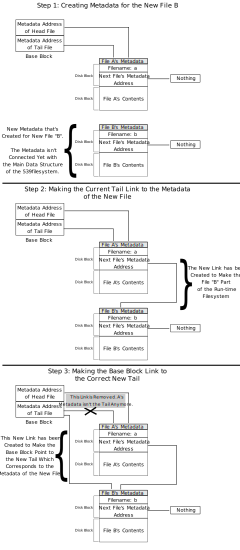
\includegraphics[width=0.85000\textwidth]{Figures/filesystem-ch/create_file_not_empty_case.png}
\caption{Steps Needed to Create New File in 539filesystem When Run-time
Filesystem isn't Empty}\label{fig:create_file_not_empty_case}
\end{figure}

\begin{lstlisting}[language=C]
metadata_t *load_metadata( int address )
{
    metadata_t *metadata = read_disk( address );
    
    return metadata;
}
\end{lstlisting}

Simply, it receives a disk address and assumes that the block which is
presented by this address is a metadata block. It loads this metadata to
the main memory by loading the content of the address from the disk
through the device driver function \lstinline!read_disk!. The following
is a sample of using \lstinline!create_file! to create a new file in the
run-time filesystem.

\begin{lstlisting}[language=C]
char *data = kalloc( 512 );

strcpy( data, "The content of the first file on 539filesystem" );
    
create_file( "first_file", data );
\end{lstlisting}

\subsubsection{Listing All Files}\label{listing-all-files}

To list all files on 539filesystem, the normal traversal algorithm of
linked-list can be used. In linked-list, to traverse all list's item you
need to start with the head of the list, then to reach the second item
of the list, the ``next'' field of the head can be used, and so on for
the rest of items in the linked-list. The ``next'' field is the
component which links the items of the list with each other. You keep
traversing the items until the tail of the list is reached and you can
check whether the current item is the tail or not by checking its
``next'' field, in case its value is \lstinline!0! (or usually in
higher-level implementations \lstinline!NULL!) then you know that the
current item is the tail which means the list is over. Another way to
check if the current item is the tail is by comparing its address with
the one which is stored in the tail field of the linked-list, in our
case, the base block. The following is the code of the function
\lstinline!list_files! which uses the algorithm we just described, it
returns an array of strings, each item of this array is a filename.

\begin{lstlisting}[language=C]
char **list_files()
{
    // Part 1
    
    if ( base_block->head == 0 )
        return -1;
    
    // Part 2
    
    char **list;
    
    list = kalloc( get_files_number() * sizeof( char * ) );
    
    // Part 3
    
    metadata_t *curr_file = load_metadata( base_block->head );
    
    int idx = 0;
    
    while ( 1 )
    {
        list[ idx ] = curr_file->filename;

        if ( curr_file->next_file_address == 0 )
            break;
        
        curr_file = load_metadata( curr_file->next_file_address );
        
        idx++;
    }
    
    return list;
}
\end{lstlisting}

The first part of \lstinline!list_files! handles the case where the
run-time filesystem is empty, so, it returns \lstinline!-1! to indicate
that there is no files to list. In case that the run-time filesystem
isn't empty, the function in the second part allocates a space in
kernel's heap for the list of the filenames, as you can see, we have
used a function named \lstinline!get_files_number! to decide how many
bytes we are going to allocate for this list, based on its name, this
function returns the number of files in the run-time filesystem, its
code will be presented in a moment. In the third part, the function is
ready to traverse the list of files metadata which are stored in the
disk and are reachable starting from the disk address which is stored in
the head field in the base block.

Initially, the metadata of the head file is loaded into memory and can
be accessed through the local variable \lstinline!curr_file!, then, the
loop is started. In the body of the loop, the filename of the current
file metadata is appended to the result's variable \lstinline!list!, in
the first iteration of this loop the filename will be the one that
belong to the head file. After appending the filename of the current
file to \lstinline!list!, the function checks if the current file is the
tail file or not by checking the value of the ``next'' field
\lstinline!next_file_address!, if it is \lstinline!0! then the current
file is the tail, so, the loop should break and the result should be
returned to the caller. In case that the current file isn't the tail
file, then the metadata of the next file is loaded by using the disk
address which is stored in the ``next'' field of the current file, the
current value of \lstinline!curr_file! is replaced with a memory address
that points to the metadata of the next file which will be used in the
next iteration of the loop, the same operation continues until the
function reaches the tail which breaks the loop and returns the list to
the caller. The following is the code of \lstinline!get_files_number!
that was used in \lstinline!list_files! and, as mentioned earlier,
returns the number of stored files.

\begin{lstlisting}[language=C]
int get_files_number()
{
    if ( base_block->head == 0 )
        return 0;
    
    int files_number = 0;
    
    // ... //
    
    metadata_t *curr_file = load_metadata( base_block->head );
    
    while ( 1 )
    {
        files_number++;

        if ( curr_file->next_file_address == 0 )
            break;
        
        curr_file = load_metadata( curr_file->next_file_address );
    }
    
    return files_number;
}
\end{lstlisting}

As you can see, it works in a similar way as \lstinline!list_files!, the
main difference is that \lstinline!get_files_number! keep tracking the
number of iterations to fetch the number of files instead of copying the
filename of the current file to another list. The following is a sample
of using \lstinline!list_files!.

\begin{lstlisting}[language=C]
void print_fs()
{
    char **files = list_files();

    for ( int currIdx = 0; currIdx < get_files_number(); currIdx++ )
    {
        print( "File: " );
        print( files[ currIdx ] );
        println();
    }
    
    print( "==" );
    println();
}
\end{lstlisting}

\subsubsection{Reading a File}\label{reading-a-file}

The function \lstinline!read_file! reads the content of a file which its
name is passed as a parameter, then, the address of the buffer that
stores that content of the file is returned to the caller. Because the
file size in 539filesystem is always \lstinline!512! bytes then
\lstinline!read_disk! of ATA device driver can be called just one time
to load a file.

To implement \lstinline!read_file!, the main thing to do is to find the
disk address of the file that the caller passed its name as a parameter,
after knowing how to traverse the list of files in 539filesystem, we can
easily use this algorithm to find the disk address of a file given its
name. The following is the code of \lstinline!read_file!.

\begin{lstlisting}[language=C]
char *read_file( char *filename )
{
    int address = get_address_by_filename( filename );
    
    if ( address == 0 )
        return 0;

    char *buffer = read_disk( address + 1 );
    
    return buffer;
}
\end{lstlisting}

The task of finding the disk address of the file's metadata is performed
by the function \lstinline!get_address_by_filename! which we will define
in a moment. When the metadata of the file is not found,
\lstinline!read_file! returns \lstinline!0!, otherwise, the file will be
read by calling \lstinline!read_disk!, as you can see, the parameter
that is passed to this function is \lstinline!address + 1! since the
value of \lstinline!address! is the disk address of the file's metadata
and not its content. Finally, the address of the buffer is returned to
the caller. The following is the code of
\lstinline!get_address_by_filename!.

\begin{lstlisting}[language=C]
int get_address_by_filename( char *filename )
{
    metadata_t *curr_file = load_metadata( base_block->head );
    int curr_file_address = base_block->head;
    
    int idx = 0;
    
    while ( 1 )
    {
        if ( strcmp( curr_file->filename, filename ) == 1 )
            return curr_file_address;
            
        if ( curr_file->next_file_address == 0 )
            break;
        
        curr_file_address = curr_file->next_file_address;
        curr_file = load_metadata( curr_file->next_file_address );      
    }
    
    return 0;
}
\end{lstlisting}

This function receives a filename as a parameter, then, it traverse the
list of the files, with each iteration, the name of the current file is
compared to the passed filename by using the function \lstinline!strcmp!
that we already defined, if the name of the current file doesn't match
the passed filename, the function loads the metadata of the next file by
using \lstinline!load_metadata! and continues to the next iteration of
the loop to check whether the next file is the required file or not, and
so on, if the file isn't found, then the loop exits and \lstinline!0! is
returned. When a match is found, the disk address of the current file's
metadata which is stored in the local variable
\lstinline!curr_file_address! is returned to the caller. The following
is a sample of using \lstinline!read_file!.

\begin{lstlisting}[language=C]
print( read_file( "first_file" ) );
\end{lstlisting}

\subsubsection{Deleting a File}\label{deleting-a-file}

As in creating a file, deleting a file may cause modifications on the
base block or even on another file's metadata. Given a filename, the
function \lstinline!delete_file! deletes this file from the run-time
filesystem, technically, the content of the file will not be overwritten
with zeros for example, instead, only the reference to this file is
removed from either the base block in case that file is the head, from
another file's ``next'' field or both in case that is file is the tail.

As mentioned earlier, this design decision of not overwriting the
content of the file, that the user would like to delete, with zeros for
example on the disk is taken in real-world filesystems to make the
delete process faster and this decision made it possible for deleted
files recovery software to exist, this type of software can recover
deleted files since their contents are still on the disk but there is
not reference to them in the run-time filesystem's data structure,
however, the space of deleted files are considered as free space by the
filesystem and it can be used anytime, that's why the recovery software
cannot ensure you that it could recover all deleted files because the
space which was occupied by the deleted file (or part of it) may be now
used by another file. The following is the code of
\lstinline!delete_file!.

\begin{lstlisting}[language=C]
void delete_file( char *filename )
{   
    // Part 1
    
    int curr_file_address = get_address_by_filename( filename );
    
    if ( curr_file_address == 0 )
        return;
    
    metadata_t *curr_file_metadata = read_disk( curr_file_address );
    
    // Part 2
    
    if ( get_files_number() == 1 )
    {
        update_base_block( 0, 0 );
        
        return;
    }
    
    // Part 3
    if ( curr_file_address == base_block->head )
    {
        update_base_block( curr_file_metadata->next_file_address, base_block->tail );
    }
    // Part 4
    else
    {
        int prev_file_address = get_prev_file_address( curr_file_address );
        
        metadata_t *prev_file = load_metadata( prev_file_address );

        prev_file->next_file_address = curr_file_metadata->next_file_address;
        
        write_disk( prev_file_address, prev_file );
        
        if ( curr_file_address == base_block->tail )
            update_base_block( base_block->head, prev_file_address );
    }
}
\end{lstlisting}

The first part tries to find the metadata address of the file in
question by using the function \lstinline!get_address_by_filename!, in
case the file is not found, the function does nothing and returns.
Otherwise, the metadata of the file is loaded and the local variable
\lstinline!curr_file_metadata! is used to point to that metadata in the
main memory.

In the second part, the most basic case of deleting a file is handled,
when there is only one file in the run-time filesystem, nothing need to
be done but updating the base block to indicate that the disk address of
both head and tail is \lstinline!0! which means, as mentioned earlier,
that the run-time filesystem is empty. The function
\lstinline!update_base_block! is used to update the base block. Figure
\ref{fig:delete_file_one_file_case} shows this case.

\begin{figure}
\centering
\includegraphics[width=0.80000\textwidth]{Figures/filesystem-ch/delete_file_one_file_case.png}
\caption{The State 539filesystem After Removing the Only
File}\label{fig:delete_file_one_file_case}
\end{figure}

The third part handles the case where the file to be deleted is the head
file, in this case, to remove the reference of this file, we simply
replace the current value of the \lstinline!head! in base block with the
metadata address of the file right next to the head which can be found
in the ``next'' field of the current head, so, the second file will
become the head file after finishing the delete process. Figure
\ref{fig:delete_file_head_case} shows this case.

\begin{figure}
\centering
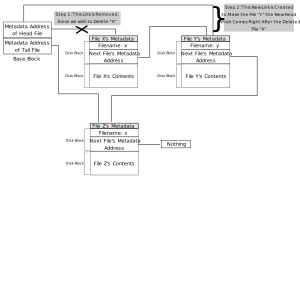
\includegraphics[width=1.00000\textwidth]{Figures/filesystem-ch/delete_file_head_case.png}
\caption{The Steps Needed to Delete the Head File in
539filesystem}\label{fig:delete_file_head_case}
\end{figure}

The fourth part of the function handles the case where the file to be
deleted is not the head, in this case, the previous file's metadata
needs to be found to modify its ``next'' field by replacing it with the
value of the ``next'' field of the file that we would like to delete, in
this way, we will be sure that the reference of the file to be deleted
is removed from 539filesystem data structure, and that the previous file
is linked with the next file. Figure \ref{fig:delete_file_not_head_case}
shows this case. Also, in this case, the file in question may be the
tail, therefore, the tail on the base block should be replaced with the
disk address of the previous file's metadata. Figure
\ref{fig:delete_file_not_head_but_tail_case} shows this case.

\begin{figure}
\centering
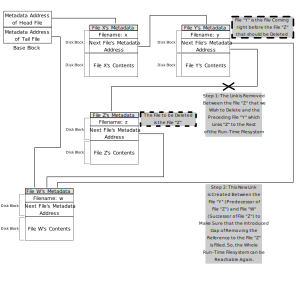
\includegraphics[width=1.00000\textwidth]{Figures/filesystem-ch/delete_file_not_head_case.png}
\caption{The Steps Needed to Delete a File which is not the
Head}\label{fig:delete_file_not_head_case}
\end{figure}

\begin{figure}
\centering
\includegraphics[width=1.00000\textwidth]{Figures/filesystem-ch/delete_file_not_head_but_tail_case.png}
\caption{The Steps Needed to Delete a File which is not the Head but
it's a Tail in 539filesystem. The File to Delete Here is
``W''.}\label{fig:delete_file_not_head_but_tail_case}
\end{figure}

As you can see in the first code line of this fourth part, a function
named \lstinline!get_prev_file_address! is used to get the disk address
of previous file's metadata to be able to perform the described
operation. By using this address, the metadata is loaded by using
\lstinline!load_metadata! in order to modify the ``next'' field of the
previous file, the updated metadata is written on the same address in
the disk. Finally, the function checks if the file to be deleted is the
tail file or not, if this is the case, the tail in base block is updated
to point to the previous file which ensures that there is no any
reference to that file in the filesystem's data structure. The following
is the code of \lstinline!get_prev_file_address! which needs no more
explanation.

\begin{lstlisting}[language=C]
int get_prev_file_address( int address )
{
    metadata_t *prev_file = load_metadata( base_block->head );
    int prev_file_address = base_block->head;

    while ( 1 )
    {
        if ( prev_file->next_file_address == address )
            return prev_file_address;
        
        prev_file_address = prev_file->next_file_address;
        prev_file = load_metadata( prev_file->next_file_address );
    }
        
    return -1;
}
\end{lstlisting}

\section{\texorpdfstring{Finishing up Version \texttt{NE} and Testing
the
Filesystem}{Finishing up Version NE and Testing the Filesystem}}\label{finishing-up-version-ne-and-testing-the-filesystem}

And now version \lstinline!NE! of 539kernel is ready. It contains a
basic ATA device driver and 539filesystem. The following is its
\lstinline!Makefile! which adds the new files to the compilation list,
also, this time we are going to use Bochs instead of QEMU to test
539filesystem since \lstinline!kernel.img! which represents the hardisk
is tailored for the former.

\begin{lstlisting}[language=make]
ASM = nasm
CC = gcc
BOOTSTRAP_FILE = bootstrap.asm 
SIMPLE_KERNEL = simple_kernel.asm
INIT_KERNEL_FILES = starter.asm
KERNEL_FILES = main.c
KERNEL_FLAGS = -Wall -m32 -c -ffreestanding -fno-asynchronous-unwind-tables -fno-pie
KERNEL_OBJECT = -o kernel.elf

build: $(BOOTSTRAP_FILE) $(KERNEL_FILE)
    $(ASM) -f bin $(BOOTSTRAP_FILE) -o bootstrap.o
    $(ASM) -f elf32 $(INIT_KERNEL_FILES) -o starter.o 
    $(CC) $(KERNEL_FLAGS) $(KERNEL_FILES) $(KERNEL_OBJECT)
    $(CC) $(KERNEL_FLAGS) screen.c -o screen.elf
    $(CC) $(KERNEL_FLAGS) process.c -o process.elf
    $(CC) $(KERNEL_FLAGS) scheduler.c -o scheduler.elf
    $(CC) $(KERNEL_FLAGS) heap.c -o heap.elf
    $(CC) $(KERNEL_FLAGS) paging.c -o paging.elf
    $(CC) $(KERNEL_FLAGS) ata.c -o ata.elf
    $(CC) $(KERNEL_FLAGS) str.c -o str.elf
    $(CC) $(KERNEL_FLAGS) filesystem.c -o filesystem.elf
    ld -melf_i386 -Tlinker.ld starter.o kernel.elf screen.elf process.elf scheduler.elf heap.elf paging.elf ata.elf str.elf filesystem.elf -o 539kernel.elf
    objcopy -O binary 539kernel.elf 539kernel.bin
    dd if=bootstrap.o of=kernel.img
    dd seek=1 conv=sync if=539kernel.bin of=kernel.img bs=512 count=20
    dd seek=21 conv=sync if=/dev/zero of=kernel.img bs=512 count=2046
    bochs -f bochs
\end{lstlisting}

To run Bochs, it should be configured properly. As you can see from the
presented \lstinline!Makefile!, a file named \lstinline!bochs! is passed
to Bochs to use it as a configuration file, so, by using it we don't
need to configure Bochs everytime we use it to run 539kernel. The
following is the content of \lstinline!bochs! file which should reside
in the same directory of 539kernel's code.

\begin{lstlisting}
plugin_ctrl: unmapped=1, biosdev=1, speaker=1, extfpuirq=1, parallel=1, serial=1, gameport=1, iodebug=1
config_interface: textconfig
display_library: x, options="gui_debug"
memory: host=32, guest=32
romimage: file="/usr/share/bochs/BIOS-bochs-latest"
vgaromimage: file="/usr/share/bochs/VGABIOS-lgpl-latest"
boot: disk
ata0: enabled=1, ioaddr1=0x1f0, ioaddr2=0x3f0, irq=14
ata0-master: type=disk, mode=flat, translation=auto, path="kernel.img", cylinders=2, heads=16, spt=63, biosdetect=auto, model="Generic 1234"
pci: enabled=1, chipset=i440fx
vga: extension=vbe, update_freq=5
cpu: count=1, ips=4000000, model=bx_generic, reset_on_triple_fault=1, cpuid_limit_winnt=0, ignore_bad_msrs=1, mwait_is_nop=0
cpuid: family=6, model=0x03, stepping=3, mmx=1, apic=xapic, sse=sse2, sse4a=0, sep=1, aes=0, xsave=0, xsaveopt=0, movbe=0, adx=0, smep=0, avx=0, avx_f16c=0, avx_fma=0, bmi=0, xop=0, tbm=0, fma4=0, vmx=1, x86_64=1, 1g_pages=0, pcid=0, fsgsbase=0, mwait=1
cpuid: vendor_string="GenuineIntel"
cpuid: brand_string="              Intel(R) Pentium(R) 4 CPU        "
\end{lstlisting}

As you can see, it tells Bochs the specifications of the virtual machine
we would like to run, also, the file which represents the hard disk
\lstinline!kernel.img! is passed to Bochs here. The following code can
be used to test 539filesystem. It should be inside
\lstinline!kernel_main! after the initializations and processes
creations.

\begin{lstlisting}[language=C]
    char *data = kalloc( 512 );
    strcpy( data, "The content of the first file on 539filesystem" );   
    create_file( "first_file", data );
    
    // ... //
    
    char *data2 = kalloc( 512 );
    strcpy( data2, "SECOND FILE in 539filesystem" );
    create_file( "second_file", data2 );
    
    // ... //
    
    char *data3 = kalloc( 512 );
    strcpy( data3, "THIRD FILE in 539filesystem" );
    create_file( "third_file", data3 );
        
    // ... //
    
    print( read_file( "first_file" ) ); println();
    print( read_file( "second_file" ) ); println();
    print( read_file( "third_file" ) ); println();
    
    // ... //
    
    print_fs();
    delete_file( "first_file" );
    print_fs();
\end{lstlisting}

This code creates three files, prints their contents, prints the
run-time filesystem tree through the function \lstinline!print_fs! and
finally deletes the file \lstinline!first_file! then prints the run-time
filesystem tree again to show that the file has been deleted
successfully. The function \lstinline!print_fs! already defined in this
chapter. To make everything works file, you need to keep the definition
of \lstinline!print_fs! below \lstinline!kernel_main! and put the
prototype \lstinline!void print_fs();! above \lstinline!kernel_main!.
Also, to test the filesystem you need to make sure that the interrupts
are disabled, the easiest way to do that is modifying
\lstinline!starter.asm! by commenting the line \lstinline!sti! which is
before \lstinline!call kernel_main! in the routine
\lstinline!start_kernel!. After that you should see the result of the
above testing code after the kernel boots up.

    \include{generated_tex/Chapter 7: What's Next?}
    \chapter*{References}\label{references}

\begin{itemize}
\tightlist
\item
  GNU Make Manual:
  \url{https://www.gnu.org/software/make/manual/make.html}
\item
  Netwide Assembler Manual:
  \url{https://www.nasm.us/xdoc/2.14.02/html/nasmdoc0.html}
\item
  Write Great Code Volume 1: Understanding the Machine.
\item
  Intel's x86 Manual.
\item
  Operating Systems Development - 8259A PIC Microcontroller by Mike,
  2007 \url{http://brokenthorn.com/Resources/OSDevPic.html}
\item
  Program and Data Representation: Textbook by Aaron Bloomfield
  \url{https://aaronbloomfield.github.io/pdr/book/index.html}
\item
  Wikipedia: x86 calling conventions
  \url{https://en.wikipedia.org/wiki/X86_calling_conventions}
\item
  Wikipedia: Interrupt request (PC architecture)
  \url{https://en.wikipedia.org/wiki/Interrupt_request_(PC_architecture)}
\end{itemize}

\end{document}
